\documentclass[12pt,oneside,spanish]{book}
\usepackage[utf8]{inputenc}

\usepackage[usenames]{color}
\definecolor{MyDarkBlue}{rgb}{0,0.4,0.65}
\usepackage[colorlinks=true,linkcolor=black,citecolor=blue,urlcolor=MyDarkBlue]{hyperref}

\usepackage{setspace}
\onehalfspacing

\usepackage{times}
\usepackage{longtable}
\usepackage[hang,small]{caption}
\usepackage{colortbl}
\usepackage{multirow}

% Márgenes y cabecera
\usepackage[letterpaper,left=3cm,right=2cm,top=3cm,bottom=2cm,includeheadfoot]{geometry}
\usepackage{fancyhdr}
\pagestyle{fancy}
\renewcommand{\headrulewidth}{1pt}
\makeatletter
\renewcommand{\chaptermark}[1]{\markboth{\textsc{\@chapapp}\ \thechapter:\ #1}{}}
\makeatother

\usepackage{amsmath} %Never write a paper without using amsmath for its many new commands
\usepackage{amssymb} %Some extra symbols
\usepackage{graphicx} %Paquete para incluir imágenes

\usepackage[activeacute,spanish]{babel}

\usepackage{apacite}
\usepackage{natbib}
\bibliographystyle{apacite}

\newcommand{\titulo}{DISEÑO E IMPLEMENTACIÓN DE UN SISTEMA DE MANEJO DEL APRENDIZAJE A DISTANCIA: ÓSMOSIS 2}
\newcommand{\autores}{ANA GABRIELA DÍAZ \\ JOSÉ LORENZO RODRÍGUEZ \\ JOAQUÍN WINDMÜLLER \\}
\newcommand{\juradouno}{Prof. Adelaide Bianchini}
\newcommand{\juradodos}{Prof. Elías Tahhan}
\newcommand{\tutor}{Prof. Fidel Gil}

\hbadness 10000
\setlength{\headheight}{15.5pt}

\hyphenation{movimiento}
\hyphenation{accesi-ble}
\hyphenation{des-habilitadas}
\hyphenation{CakePHP}

%Para resaltar código en php
\usepackage{listings}

\definecolor{light-gray}{gray}{0.97}
\definecolor{keyword}{rgb}{0.47, 0.53, 0.6}
\definecolor{string}{rgb}{0.73, 0.53, 0.27}
\definecolor{comment}{rgb}{0.6, 0.6, 0.53}

\lstset{
  columns=fixed,
  basicstyle=\footnotesize\ttfamily,
  identifierstyle=\color{black},
  keywordstyle=\color{keyword},
  stringstyle=\color{string},
  commentstyle=\color{comment}\itshape,
  backgroundcolor=\color{light-gray},
  frame=single,
  framerule=0pt,
  breaklines,
  showstringspaces=false,
  tabsize=4
}

\lstdefinelanguage{PHP}
  {morekeywords={
    % Case-sensitive keywords:
    abstract,and,as,break,case,catch,class,const,continue,default,die,do,echo,
    else,elseif,endfor,endforeach,endswitch,endwhile,extends,for,global,final,
    foreach,function,if,implements,import,include,include_once,instanceof,
    interface,list,namespace,new,or,print,private,protected,public,require,
    require_once,return,static,switch,throw,try,var,while,xor,Configure,
    % Case-insensitive keywords:
    true,True,TRUE,false,False,FALSE,null,Null,NULL},
   morekeywords=[2]{
     array,bool,boolean,double,float,int,integer,object,real,string,unset},
   otherkeywords={-,.,~,^,@,;,:,\%,|,=,+,!,?,&,<,>},
   sensitive=true,
   morecomment=[l]{//},      % C++ line comment
   morecomment=[l]{\#},      % Bash line comment
   morecomment=[s]{/*}{*/},  % C block comment
   morestring=[b]{'},        % single-quoted string
   morestring=[b]{"}         % double-quoted string
  }

% \includeonly{caracteristicas_sistema}


\newsavebox{\mygraphic}
\sbox{\mygraphic}{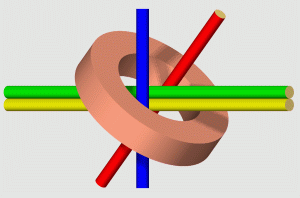
\includegraphics[keepaspectratio,
height=0.1\textheight, width=0.1\textwidth]{imagenes/escudo.png}}
\pagestyle{fancy}
\fancyhead{}
\fancyhead[L]{\setlength{\unitlength}{1in}
\fancyhead[C]{Escuela de Especialidades Antonio de Escaño \\ Departamento TCI - Informática}
\fancyhead[R]{\thepage} % Número arriba a la derecha 
\begin{picture}(0,0)
  \put(0,0){\usebox{\mygraphic}}
\end{picture}}
%\renewcommand{\footrulewidth}{0.4pt}
%\fancyfoot[L]{\setlength{\unitlength}{1in}
%\fancyfoot[C]{UNIX}
%\fancyfoot[R]{\thepage}





\begin{document}

%!TEX root = Libro.tex
\begin{titlepage}
\vspace{2cm}
\begin{Large}
	\begin{center}
		
\includegraphics{imagenes/cebolla.png} \\
		UNIVERSIDAD SIMÓN BOLÍVAR \\
		Ingeniería de la Computación.
	\end{center}
\end{Large}
\vspace{2cm}
\begin{Large}
	\begin{center}
		\textbf{\titulo}
	\end{center}
\end{Large}
\vspace{1cm}
\begin{large}
	\begin{center}
		Por \\
		\autores
	\end{center}
\end{large}
\vspace{2cm}
\begin{large}
	\begin{center}
		Proyecto de Grado  \\ 
		Presentado ante la Ilustre Universidad Simón Bolívar \\
		como Requisito Parcial para Optar el Título de \\
		Ingeniero en Computación \\
		\vspace{1cm}
		Sartenejas, \today
	\end{center}
\end{large}
\end{titlepage}
\newpage

\pagestyle{empty}
%!TEX root = Libro.tex
\begin{center}
	
\includegraphics{imagenes/cebolla.png} \\
	UNIVERSIDAD SIMÓN BOLÍVAR \\
	DECANATO DE ESTUDIOS PROFESIONALES \\
	COORDINACIÓN DE INGENIERÍA DE LA COMPUTACIÓN \\
	\vspace{0.5cm}
	ACTA FINAL DEL PROYECTO DE GRADO \\
	\vspace{0.4cm}
	\textbf{\titulo} \\
	\vspace{0.5cm}
	Presentado por: \\
	\autores
	\vspace{0.6cm}
	Este Proyecto de Grado ha sido aprobado por 
	el siguiente jurado examinador: \\
	\vspace{0.6cm}
	
	----------------------------------------- \\
	\juradouno \\
	Jurado \\
	\vspace{1cm}
	
	----------------------------------------- \\
	\juradodos \\
	Jurado \\
	\vspace{1cm}
	
	----------------------------------------- \\
	\tutor \\
	Tutor \\
	\vspace{0.4cm}
	Sartenejas, \today
\end{center}
\newpage

%!TEX root = Libro.tex
\begin{large}
	\begin{center}
		\textbf{\titulo}
	\end{center}
\end{large}
\begin{large}
	\begin{center}
		Por \\
		\autores
	\end{center}
\end{large}

\begin{center}
	\textbf{RESUMEN}
\end{center}

Con la masificación del acceso a la tecnología, y en especial a Internet, la labor pedagógica se ha visto en la obligación de ponerse al día con las nuevas herramientas existentes, no solo con la intención de garantizar una máxima asimilación de los contenidos, sino también para extender la labor educativa a personas que, anteriormente, no tenían acceso al conocimiento.\\

La nueva tendencia en el uso de Internet, denominada Web2.0, apuntan a que los sitios más exitosos serán aquellos que logren aprovechar la inteligencia colectiva para generar contenidos con valor agregado. Pero para alcanzar ese conocimiento colectivo es necesario alcanzar masa crítica, para lograrlo es necesario ofrecer un servicio de alta calidad y en constante evolución.\\

Implementar esta nueva tendencia en un entorno de aprendizaje en línea es el principal objetivo del presente proyecto de grado. Partiendo de la plataforma existente en la Universidad Simón Bolívar, se plantea desarrollar su reestructuración de modo que se convierta en un repositorio navegable del conocimiento organizacional generado dentro del campus.\\

La meta de este trabajo fue la implementación de un Sistema de Manejo del Aprendizaje (LMS, por sus siglas en inglés), que ofrezca a la comunidad universitaria un entorno educativo con las características propias de la Web2.0 y a sus administradores un entorno de fácil mantenimiento que permita el rápido crecimiento y evolución por medio del desarrollo de nuevas funcionalidades.\\

Ósmosis2, como se denomina este proyecto, ofrecerá a los estudiantes y profesores una nueva forma de aprender y de dejar un legado a toda la comunidad.


\pagenumbering{roman}
\tableofcontents
\newpage
\listoftables
\newpage
\listoffigures
\newpage
% libro
\pagenumbering{arabic}

\pagestyle{plain}
%!TEX root = Libro.tex
\section*{Introducción}
\addcontentsline{toc}{section}{Introducción}
Con la masificación del acceso a la tecnología, y en especial a Internet, la labor pedagógica se ha visto en la obligación de ponerse al día con las nuevas herramientas existentes, no solo con la intención de garantizar una máxima asimilación de los contenidos, sino también para extender la labor educativa a personas que, anteriormente, no tenían acceso al conocimiento.\\

La Universidad Simón Bolívar no ha sido la excepción; aprovechando el acceso masivo a Internet como herramienta viable y de bajo costo para implantar una plataforma que sirva como complemento para los cursos que se dictan en sus aulas. En la actualidad, la institución cuenta con un portal educativo basado en un ambiente Web, la cual brinda apoyo al docente en la entrega de material complementario y acercamiento a los alumnos de los cursos que dicta.\\

Este es el camino que han tomado, con mayor o menor éxito, muchas otras entidades educativas alrededor del mundo. El software que apoya estas plataformas se ha ido desarrollando sobre la marcha, conforme las necesidades hayan ido demandando nueva funcionalidades, y los avances tecnológicos así lo hayan permitido. Pero en gran parte han sido desarrollados sin una concepción previa de cómo deben ser utilizados estos nuevos recursos para sacar el mayor provecho pedagógico a los mismos.\\

En la actualidad el área de mayor auge en Internet son las comunidades, en donde grupos de usuarios que se dedican a compartir contenidos multimedia los cuales pueden comentar, calificar y clasificar; fenómeno que algunos han llamado ``Web 2.0''. Este modelo de interacción, en el cual el usuario es generador de contenidos, se ha probado a si mismo y a sus usuarios como muy útil, puesto que se aprovecha al máximo la capacidad de comunicación, casi instantánea, que brinda la tecnología para la generación de información valiosa a la que todos pueden acceder.\\

Surge entonces la siguiente pregunta, ¿por qué no usar este modelo para facilitar la labor educativa? Parte de la respuesta contempla el evaluar el uso que se le está dando a las plataformas que ya se poseen e intentar adaptarlas a este nuevo enfoque.\\

El presente proyecto nace de dicha necesidad de replantear las herramientas utilizadas actualmente por la Universidad Simón Bolívar, de manera que estas se transformen en facilitadores al servicio de quienes van a utilizarlas y se adecuen lo mejor posible a las estructuras que se manejan en el ambiente educativo, abriendo paso, a su vez, al nuevo paradigma de la educación a distancia.\\

Para ello se requiere evaluar y seleccionar aquellos componentes que mejor se adapten al nuevo ambiente de aprendizaje y que a su vez estimulen no sólo la adquisición de conocimientos, sino la generación de los mismos. Con esto, es posible plantear un nuevo enfoque que supone hacer más énfasis en la comunidad de usuarios (estudiantes y profesores) que en los contenidos, sin descuidar la calidad de los últimos y que, además, busca reflejar, virtualmente, la interacción física que se observa en las aulas de clase.\\

\pagestyle{fancy}
%!TEX root = Libro.tex
\chapter{Planteamiento del Problema}
\section{Antecedentes}
La Web lentamente ha pasado de ser un mero mecanismo de entrega de contenidos, a ser una plataforma de intercambio virtualmente presente en cualquier computador. Esto la ha convertido en la opción clara para la implementación de soluciones vinculadas a la creciente necesidad de emplear nuevas tecnologías como medio de apoyo a la educación tradicional.\\

Sin embargo, la educación a distancia, también llamada \emph{e-learning}, ha evolucionado a un ritmo mucho más lento que otras áreas en la Web, posiblemente por tratar de aplicar a la misma modelos que tradicionalmente han sido válidos para la educación presencial. Los sistemas de educación a distancia, en su mayoría, se encuentran atados a la filosofía lectura/escritura con la cual nació la Internet, haciendo que el intercambio de información sea unidireccional; paradigma que día a día se hace menos atractivo.\\

A esta tendencia se le agrega, como lo indica un estudio hecho en la USB, el desinterés de de los docentes por conocer y aplicar estrategias de educación a distancia. De dicho estudio se concluyó que era necesario \emph{``dar a conocer metodologías y herramientas para la creación de cursos a distancia''}, incluyendo la adopción de estándares que promuevan \emph{``la portabilidad, accesibilidad e interoperabilidad de los recursos educativos [...] trayendo consigo el efecto de mejorar cualquier iniciativa que se desee en la creación de cursos a distancia''} \citep{Diaz2007}\\

Este desinterés es un fenómeno generalizado que afecta a las plataformas educativas, y que se hace mucho más evidente cuando se las  compara con las actuales herramientas masivas de intercambio de información que han emergido de una nueva cultura en la Internet. Para muchas de estas plataformas la solución ha sido agregar nuevas capacidades para mantener la paridad con las nuevas tendencias. Sin embargo, este crecimiento ha generado una desconexión entre las herramientas y los beneficios pedagógicos que persiguen, y más importante aún, han olvidado mantener la motivación del alumno/docente para utilizar la aplicación.

\section{Ósmosis 1.5}
Para las organizaciones que contemplan al \emph{e-learning} como una parte fundamental de su trabajo, las principales necesidades se encuentran en lograr un proceso sostenido de creación de información, y la evolución de la plataforma ante los requerimientos de sus usuarios. De allí se desprende que las funcionalidades que se requieren para un sistema de este tipo sean la transferencia rápida y efectiva de conocimiento, el enriquecimiento de la información a través de su contexto y la habilidad de fabricar contenidos educativos en menos tiempo y con el menor costo posible \cite{Karrer2007}.\\

Esas mismas necesidades fueron las que llevaron a la Dirección de Servicios Multimedia (DSM) a iniciar la construcción de una plataforma educativa. A continuación se presenta una sinopsis de la evolución que siguió el proyecto hasta llegar a la plataforma con la que cuenta actualmente.\\

Este proyecto tiene su origen en una necesidad personal del jefe de la sección Web de la DSM, Hermes Rodríguez, mientras cursaba la Especialización en Telecomunicaciones: habilitar un espacio para compartir la mayor cantidad de información posible con sus compañeros de clase y docentes. Así surge esta primera plataforma de \emph{e-learning}, un desarrollo sencillo con funcionalidad limitada.\\ 

Posteriormente se utiliza el sistema de manejo de contenidos Claroline para hacer una propuesta formal, sin embargo luego de realizar un estudio pedagógico y tecnológico, se selecciona Dokeos -- un software de código abierto regido por la licencia GPL -- como herramienta para desarrollar la plataforma.\\

El desarrollo de nuevas funcionalidades se basó en los requerimientos específicos de los usuarios. Dichos aditamentos fueron propuestos a los desarrolladores de Dokeos bajo el espíritu de la GNU/GPL. Sin embargo dichos aportes no fueron implementados en la línea principal de desarrollo del paquete de \emph{e-learning}, por lo que la USB terminó, sin querer, con un nuevo producto que lentamente se alejó de la línea de desarrollo principal de Dokeos. Ante esta realidad se decidió bautizar a la nueva herramienta ``Ósmosis'' en referencia a su origen: facilitar la transferencia de conocimiento entre los actores que la utilizan. \\

Desde entonces Ósmosis ha sido promocionada desde de la Universidad Simón Bolívar para convertirla en un producto que permita generar redes de conocimiento a nivel nacional.

\subsection[Aula Virtual (USB)]{Aula Virtual de la Universidad Simón Bolívar}
La única implantación conocida, en producción, de Ósmosis se encuentra en la Universidad Simón Bolívar y es la plataforma de aprendizaje a distancia, conocida como Aula Virtual, que sirve tanto a los cursos regulares como a los de extensión y a algunos liceos de la zona. En números, a la fecha (29/01/2008) Ósmosis ofrece su servicio a \textbf{22.311 usuarios}, de los cuales \textbf{647 son docentes}. Se manejan \textbf{1.274 cursos} (882 públicos y 392 privados) en \textbf{35 categorías}. El \textbf{curso más antiguo} fue creado el \textbf{13 de Septiembre de 2004} y el mas reciente data del \textbf{29 de Enero de 2008}.\\

La cantidad de usuarios del sistema demuestra que además de los miembros de la comunidad de la Universidad Simón Bolívar también participan otras entidades educativas, por ejemplo, el curso con más estudiantes inscritos (\textbf{594}) es Introducción a la Informática y se dicta en la UNEFA (Universidad Experimental Politécnica de la Fuerza Armada Bolivariana).

\subsubsection{Deficiencias}
A pesar del éxito que ha tenido la implementación de Ósmosis en las Aulas Virtuales, es importante reconocer que Ósmosis tiene su origen en Dokeos, el cual carecía de una buena documentación y ha heredado código e ideas de distintos Sistemas de Gestión del Aprenizaje (SGA o LMS, por sus siglas en inglés) por lo que actualmente presenta un código fuente difícil de mantener.\\

A nivel técnico, Ósmosis está desarrollado en PHP, sin la utilización de algún \emph{framework}, y carece de una separación clara entre las capas lógica/datos/vista lo cual, en el mejor de los casos, hace que el desarrollo de nuevas funcionalidades o la solución de problemas sea ineficiente.

\section{Ósmosis2}
Este proyecto, al que se denominará indiscriminadamente Ósmosis2 y Ósmosis2, surge como consecuencia de lo expuesto anteriormente, con la finalidad de contemplar y llevar a cabo el diseño e implementación de una nueva versión de Ósmosis, en la cual sea posible incorporar nuevas tecnologías e integrarlas con los recursos pedagógicos que los docentes demandan, esto con la finalidad de que la plataforma sea empleada como herramienta principal para el aprendizaje.\\

Así mismo, y en función del crecimiento de Ósmosis, uno de los requisitos para esta nueva versión es lograr un código mantenible, lo que implica la menor cohesión posible entre sus capas. Es decir, la reingeniería de la plataforma para adaptarla a las necesidades pedagógicas y tecnológicas actuales.\\

A continuación se presentan los objetivos generales y específicos del proyecto en cuestión:

\subsection{Objetivos Generales}
\begin{itemize}
	\item Diseñar y desarrollar un Sistema de Gestión del Aprendizaje fundamentado en corrientes pedagógicas y en los principios de la Web 2.0.
	\item Desarrollar una plataforma modular de aprendizaje a distancia que se adapte a las necesidades pedagógicas actuales.
	\item Evaluar las características de la versión actual de Ósmosis.
\end{itemize}
	
\subsection{Objetivos Específicos}
\begin{itemize}
	\item Realizar una investigación referente a la definición de LMS y sus características.
	\item Estudiar los enfoques pedagógicos de mayor uso contemplados en los LMS
	\item Analizar y comparar los distintos LMS existentes.
	\item Realizar el levantamiento y análisis de los requerimientos de la plataforma, incluyendo estándares existentes en el diseño de contenidos para la educación.
	\item Establecer, a partir del análisis de los LMS y los requerimientos detectados, las funcionalidades que contemplará la plataforma de Ósmosis2
	\item Evaluar y seleccionar una plataforma de desarrollo sobre la cual se desarrollará el LMS (lenguajes, frameworks, manejadores de bases de datos, etc). 
	\item Diseñar una interfaz gráfica que permita reflejar la nueva visión de Ósmosis
\end{itemize}

\pagebreak

% -- Educación en línea --
	%!TEX root = ../Libro.tex
\chapter{Marco Teórico}
\section{Educación en Línea}
La educación en línea se refiere a a educación virtual, distribuída a través de Internet, la Web o cualquier otra forma de educación desarrollada con la mediación de las computadoras. Se caracteriza por:
\begin{itemize}
	\item Separación del maestro y el aprendiz, lo que la diferencia de la educación presencial.
	\item La influencia de una organización educativa, lo que la diferencia del aprendizaje autodidacta y de la tutoría privada.
	\item El uso de una red de computadores para presentar o distribuir los contenidos educativos.
	\item La disponibilidad de una vía de comunicación a través de una red de computadores de modo que los estudiantes se beneficien de la comunicación entre ellos y con el profesor.
\end{itemize}

A pesar de que el término \emph{e-learning} se usa como sinónimo de educación en línea, es importante aclarar que son distintos y que ``educación en línea'' es más amplio: \emph{e-learning} sólo se refiere a la entrega de los contenidos y la retroalimentación automatizada ante las actividades desarrolladas por el estudiante y no a la comunicación entre aprendiz y tutor. \citep{Paulsen2002}

\subsection{Learning Management Systems (LMS)}
Learning Management Systems o Sistema de Gestión del Aprendizaje, es un término amplio usado para referirse a sistemas que organizan y proveen acceso a servicios de aprendizaje en línea para estudiantes, educadores y administradores. Estos servicios incluyen control de acceso, fuente de contenidos de aprendizaje, herramientas de comunicación y organización en grupos de usuarios. También se les conoce como plataformas de aprendizaje \citep{Paulsen2002}.

\subsubsection{Objetivos}
Según \citeauthor{Hall2002}, algunos de los objetivos de un Sistema de Gestión del Aprendizaje (LMS) son:

\begin{itemize}
	\item Permitir la reutilización y redistribución de los contenidos.
	\item Ofrecer alta disponibilidad, y facilidad de uso mientras se mantiene la escalabilidad, la seguridad y la estabilidad.
	\item Integrar aprendizaje en los salones con aprendizaje en línea.
	\item Medir la efectividad de las iniciativas de aprendizaje mediante el seguimiento del progreso de los estudiantes y su desempeño en los distintos tipos de actividades. 
	\item Servir de contenedor de cursos.
	\item Facilitar la comunicación y el trabajo colaborativo entre profesores y estudiantes.
\end{itemize}
\citep{Hall2002}

\subsubsection {Características}
En cuanto a las características básicas que debe tener un LMS son destacables:

\begin{itemize}
	\item Administración de usuarios, roles, profesores, herramientas y generación de reportes.
	\item Calendario del curso.
	\item Mensajes y notificaciones a estudiantes.
	\item Autoevaluaciones y pruebas que permitan manejar el desempeño del estudiante antes y después de las evaluaciones
	\item Puntuación de actividades del curso, individual y por grupos, incluyendo lista de espera.
	\item Mostrar calificaciones y actas de notas.
	\item Distribución del curso a través de la Web o por medio de la misma.
\end{itemize}
\citep{Greenberg2002}
	%!TEX root = ../Libro.tex
\section{Corrientes Pedagógicas}
Las corrientes pedagógicas son distintas teorías de pensamiento, surgidas a lo largo de la historia, que intentan explicar el proceso de aprendizaje y formación del ser humano, las más importantes son:
\begin{itemize}
	\item Conductismo
	\item Cognitivismo
	\item Constructivismo
	\item Constructivismo social
	\item Conectivismo
\end{itemize}

\subsection{Conductismo}
Según \citeauthor{Conductismo_Manosalva1996}, en el conductismo la experiencia precede al conocimiento, en otras palabras, define el aprendizaje como un cambio observable en el comportamiento producto de una relación ``estímulo - respuesta''. Los procesos internos tales como el pensamiento y la motivación son incognoscibles \citep{Conductismo_Manosalva1996}, no pueden ser observados ni medidos directamente por lo que no son relevantes a la investigación científica del aprendizaje.
El aprendizaje se constata por medio de la observación de un cambio en el comportamiento. Si no hay cambio observable no hay aprendizaje.\\

El conductismo aprueba el uso de refuerzos para fortalecer conductas apropiadas y su desuso para debilitar las no deseadas. La asignación de calificaciones, recompensas y castigos son también aportaciones de esta teoría.\\

Los principios de las ideas conductistas pueden aplicarse con éxito en la adquisición de conocimientos memorísticos que suponen niveles primarios de comprensión, como por ejemplo el aprendizaje de las capitales del mundo o las tablas de multiplicar. Sin embargo esto presenta una limitación importante: la repetición no garantiza asimilación de la nueva conducta, sino sólo su ejecución. Por ejemplo, una persona puede aprender las tablas de multiplicar pero no sabrá cuando debe hacer uso de ellas. Esto indica que la situación aprendida no se puede extrapolar fácilmente a otras situaciones.\\

En este paradigma, el estudiante es un individuo cuyo aprendizaje se puede modificar por medio de un reajuste de los recursos educativos de tal manera que éste adquiera las actitudes académicas deseadas.\\

El maestro es el encargado de ejecutar dichos reajustes así como aplicar los estímulos necesarios para la enseñanza.

\subsection{Cognitivismo}
El paradigma cognitivista sustenta al aprendizaje como un proceso en el cual se sucede la modificación de significados de manera interna, producido intencionalmente por el individuo como resultado de la interacción entre la información procedente del medio y el sujeto activo. Dicha perspectiva surge a finales de 1960 como una transición entre el paradigma conductista y las actuales teorías psicopedagógicas.\\

``Al cognitivismo le interesa la representación mental y por ello las categorías o dimensiones de lo cognitivo: la atención, la percepción, la memoria, la inteligencia, el lenguaje, el pensamiento y para explicarlo puede, y de hecho acude a múltiples enfoques, uno de ellos es el de procesamiento de la información; y cómo las representaciones mentales guían los actos (internos o externos) del sujeto con el medio, pero también cómo se generan (construyen) dichas representaciones en el sujeto que conoce.'' \citep{Cognitivismo_Ferreiro1996}\\

El cognitivismo es, de manera simplificada, el proceso independiente de decodificación de significados que conduzcan a la adquisición de conocimientos a largo plazo y al desarrollo de estrategias que permitan la libertad de pensamiento, la investigación y el aprendizaje continuo en cada individuo, lo cual da un valor real a cualquier cosa que se desee aprender. De aquí entonces se desprende el paradigma del Cognitivismo, ``un marco global de referencia para el crecimiento y desarrollo personal'' \citep{Cognitivismo_Ferreiro1996}

\subsection{Constructivismo}
Esta corriente pedagógica afirma que el conocimiento de todas las cosas es un proceso mental del individuo, que se desarrolla de manera interna conforme obtiene información y se relaciona con su entorno.\\

Para el constructivismo, el aprendizaje es un proceso en el cual el estudiante construye activamente nuevas ideas o conceptos basados en conocimientos presentes y pasados. En otras palabras, ``el aprendizaje se forma construyendo nuestros propios conocimientos desde nuestras propias experiencias'' \citep{Constructivismo_Ormrod2003}\\

A pesar de ser el aprendiz quien construye su aprendizaje, el profesor juega un rol importante en el proceso, actuando como facilitador y animando a los estudiantes a solucionar problemas reales o simulaciones. Por lo general el aprendizaje se hace por medio de un proceso social de colaboración entre los estudiantes y bajo esta óptica, el proceso de aprendizaje no es de ``todo o nada'' sino que los estudiantes desarrollan nuevos conocimientos a partir de los que ya poseen. Esto significa que el docente debe constatar que el aprendizaje efectivo logrado por el aprendiz es el esperado así como fomentar la conexión entre los estudiantes y plantear situaciones para estimular el razonamiento.\\

El constructivismo propone una metodología de aprendizaje, más no propone los medios para llevar a cabo dicho aprendizaje. Es decir, describe cómo ocurre pero no cómo se logra el aprendizaje.

\subsection{Constructivismo social}
El constructivismo social en educación y teoría del aprendizaje estudia la forma en que el ser humano aprende a la luz de su situación social y de la comunidad en la que aprende.\\

Uno de los puntos focales del constructivismo es descubrir las maneras en las que los individuos y grupos participan en la creación de la percepción de su realidad social. El estudio de la aparición de fenómenos sociales, su institucionalización y como posteriormente se tornan en tradiciones. La realidad construida socialmente, por los individuos y su interpretación de sus conocimientos, es un proceso dinámico y constante. \\

En décadas recientes, los teóricos del constructivismo han extendido en enfoque tradicional del aprendizaje para referirse a las dimensiones colaborativas y sociales del aprendizaje.  \\

\citeauthor{Holmes2001}, propone extender el constructivismo social de modo que se tome en cuenta la sinergía entre los más recientes avances de la tecnología de la información. Introduce el término Constructivismo Comunal, en el cual ``los estudiantes no solamente pasan a través de un curso, como el agua a través de una tubería; sino que dejan su propia huella en el proceso de aprendizaje, en su escuela o universidad e idealmente en su disciplina. Esto resultará en un beneficio para el curso o la institución, pero más importante es el beneficio que genera a los estudiantes.'' Avances como los blogs, wikis y podcasts, aumentan el potencial comunicacional de los individuos, lo cual permite que el conocimiento construido individualmente redunde en un beneficio a los demás aprendices.\citep{Holmes2001} \\

El constructivismo social expone que el ambiente de aprendizaje óptimo es aquel donde una interacción dinámica entre los instructores y los alumnos, con actividades que proveen oportunidades para los alumnos de crear su propia verdad gracias a la interacción con lo demás. Esta teoría, por lo tanto, enfatiza la importancia de la cultura y el contexto para el entendimiento de lo que está sucediendo en la sociedad y para construir conocimiento basado en este entendimiento \citep{Carretero1997}. \\

Según \citeauthor{Glasersfeld1989}, el constructivismo social plantea dos principios fundamentales cuya aplicación tiene consecuencias tanto en el estudio del desarrollo cognitivo como en la práctica educativa:

\begin{itemize}
	\item El conocimiento no se recibe pasivamente sino que es construido activamente por el sujeto cognitivo.
	\item La función del aprendizaje es adaptable. Sirve para la organización del mundo de la experiencia y no para el descubrimiento de una realidad ontológica \citep{Glasersfeld1989}
\end{itemize}

\subsection{Conectivismo}
El conectivismo es una teoría del aprendizaje para la era digital que ha sido desarrollada por George Siemens basado en el análisis de las limitaciones del conductismo, el cognitivismo y el constructivismo, para explicar el efecto que la tecnología ha tenido sobre la manera en que actualmente vivimos, nos comunicamos y aprendemos. \citep{Conectivismo_Siemens2004}\\

El conectivismo es la integración de los principios explorados por la teorías del caos, redes neuronales, complejidad y auto-organización. El aprendizaje, según \citeauthor{Conectivismo_Siemens2004}, es un proceso que ocurre dentro de una amplia gama de ambientes que no no están necesariamente bajo el control del individuo, es por esto que el conocimiento puede residir fuera del ser humano, por ejemplo dentro de una organización o una base de datos, y se enfoca en la conexión especializada en conjuntos de información que nos permita aumentar cada vez más nuestro estado actual de conocimiento.\\

Esta teoría es conducida por el entendimiento de que las decisiones están basadas en las transformación acelerada de los basamentos. Continuamente nueva información es adquirida dejando obsoleta la anterior. En este contexto, es vital adquirir la capacidad para discernir entre lo importante y lo trivial, así como la capacidad para reconocer cuando esta nueva información altera las decisiones tomadas en base a la información pasada.\\

El punto de inicio del conectivismo es el individuo. El conocimiento personal se hace de una red, que alimenta de información a organizaciones e instituciones, que a su vez agregan nueva información en la misma red, lo cual termina proveyendo nuevo aprendizaje al individuo. Este ciclo de desarrollo del conocimiento permite a los aprendices a mantenerse actualizados en el campo en el cual han formado conexiones.

\paragraph{Principios del conectivismo}
\begin{itemize}
	\item El aprendizaje y el conocimiento yacen en la diversidad de opiniones.
	\item El aprendizaje es el proceso de conectar nodos o fuentes de información.
	\item No solo los humanos aprenden y el conocimiento puede residir fuera del ser humano.
	\item La capacidad de aumentar el conocimiento es más importante que la información conocida.
	\item Nutrir y mantener las conexiones es necesario para facilitar el aprendizaje continuo.
	\item La habilidad para ver las conexiones entre los campos, ideas y conceptos es primordial.
	\item La información actualizada y precisa es la intención de todas las actividades del proceso conectivista.
	\item La toma de decisiones es en sí misma un proceso de aprendizaje. Escoger qué aprender y el significado de la información entrante es visto a través del lente de una realidad cambiante: es posible que lo que hoy es correcto mañana esté errado bajo la nueva información que se recibe.
\end{itemize}

Con respecto al primer punto, \citeauthor{Conectivismo_Siemens2005} indica que una red de aprendizaje puede sostener puntos aparentemente contradictorios dado que lo que hoy es cierto mañana podría no serlo ante algún cambio en la base. Y es esta diversidad la aumenta la posibilidad de realizar decisiones acertadas. \citep{Conectivismo_Siemens2005}
	%!TEX root = ../Libro.tex
\subsection{Learning Objects}
Según \citeauthor{LearningOb_Beck2007}, existen 3 definiciones prominentes de qué son los learning objects:
\begin{itemize}
	\item ``Cualquier entidad, digital o no, que puede ser usado para el aprendizaje, educación o entrenamiento.''
	\item ``Cualquier recurso que puede ser reusado para dar soporte al aprendizaje''
	\item ``Una entidad digital que puede ser usada, reusada o referenciada durante el aprendizaje apoyado por la tecnología.'' 
\end{itemize}

En términos generales, sus principales características son \citep{LearningOb_Beck2007}:

\begin{itemize}
	\item \textbf{Auto-contenido y reusable}: \\ Cada learning object es independiente y puede ser compartido y reusado, en distintas ocasiones y para distintos fines, como una entidad indivisible.
	\item \textbf{Entidad de aprendizaje reducida}: \\ Al contrario de una clase completa, los learning object contienen recursos más breves de aprendizaje de unos 2 a 15 minutos.
	\item \textbf{Pueden ser agregados}: \\ Los learning objects pueden ser agrupados en colecciones más grandes, incluso en estructuras tradicionales de educación.
	\item \textbf{Rastreados con metadatos}: \\ Cada learning object contiene información descriptiva sobre la cual se pueden realizar búsquedas.
\end{itemize}
% -- Web 2.0 -- 
	%!TEX root = ../Libro.tex
\section{La Web 2.0}
El término \emph{Web 2.0} fue usado por primera vez por Dale Dougherty, vice-presidente de O'Reilly Media, en una sesión de ideas sobre el estado de la web luego de la ruptura de la ``burbuja .com'', en 2001. Dougherty notaba que la web era más importante que nunca y que las compañías que habían sobrevivido tenían muchos aspectos en común, dichas observaciones le hacían pensar que el colapso marcado por la ruptura de la burbuja determinó un punto de inflexión y que un llamado a la acción era necesario.\\

El término cobró interés desde entonces, pero hasta el momento la comunidad de desarrolladores web mantiene un desacuerdo del verdadero significado. Para zanjar de dicha diatriba, \citeauthor{Web_OReilly20052} publicó un artículo en el que aclaraba mucho de los discutido en esa sesión de ideas que dio origen al término. De dicho artículo son destacables los siete principios de la Web 2.0:

\subsection{La web como plataforma} 
\emph{Netscape Comunications}, creadores del navegador Netscape, fue la pionera en usar la web como plataforma aprovechando su dominio en el mercado de los navegadores (siendo el estandar de facto). Ofrecía un entorno (\emph{webtop}) de servicios de alto costo hospedados en el propio navegador. Al final los navegadores y los servidores se convirtieron en simple mercancía y el verdadero valor se depositó en los servicios entregados sobre la plataforma web.\\

En contraste, usando esta filosofía de entrega de servicios surgió Google. Que sin requerir instalaciones, actualizaciones o parches, ofrecía al usuario un servicio en constante mejora que generaba ganancias de manera directa o indirecta de su uso.\\

La web como plataforma se utiliza para entregar software en forma de servicios en vez de recibir servicios a través de un software.

\subsection{Aprovechando la inteligencia colectiva}
Frases como la de Eric Raymond, originalmente acuñada para referir al software de código abierto, ``con suficientes ojos, cualquier error es leve'' \citep{Neff2002} resuenan en la Web 2.0 potenciada por los usuarios: sistemas de calificación de los contenidos como el de Digg.com implementan a cabalidad la citada frase, mientras que sitios insignia de la Web 2.0 como del.icio.us y flickr.com permiten a los usuarios etiquetar los contenidos (enlaces y fotografías respectivamente) generando estructuras flexibles para la clasificación de los contenidos, denominadas folcsonomías, en contraste con las tradicionales taxonomías definidas por un administrador.

\subsection{Los datos son el próximo Intel Inside}
Todos los sitios web significativos de la actualidad se basan en el manejo de datos. Esta es la principal competencia de las iniciativas Web 2.0: el manejo de datos. La frase de Hal Varian ``SQL es el nuevo HTML'' resume la importancia que tiene el manejo de los datos.\\

Pero no sólo se trata de tener el control sobre el contenido, sino generar valor agregado a partir de dichos datos. Un ejemplo de ello es Amazon.com y Barnesandnoble.com, ambas compañías obtuvieron su catálogo de un mismo proveedor, sin embargo  Amazon se dedicó desde un comienzo a mejorar los datos agregándoles información obtenida de las casas editoriales como imágenes de las portadas, tabla de contenidos, índice y material de muestra. No sólo eso, sino que aprovecharon a sus usuarios para agregar notas a los datos de tal manera que, luego de 10 años, es Amazon y no su proveedor original quien es considerado la principal fuente para referencias bibliográficas. Adicionalmente, Amazon introdujo su propio identificador que permite referir libros que no tienen ISBN. \\ 

La carrera consiste en controlar ciertos tipos de datos: localización, identidad, fechas de eventos públicos, identificadores de productos y otros. En algunos casos el costo de crear y recopilar los datos permitirá al beneficiado mantener el control sobre ellos y licenciarlos, construyendo así lo que se denomina el Intel Inside. En los demás casos, el ganador será aquel que alcance el punto crítico por medio de sus usuarios, generando un servicio con valor agregado.

\subsection{El fin del Ciclo de Liberación del Software} 
El hecho de que el software sea entregado como servicio y no como un producto conlleva dos cambios fundamentales:

\begin{itemize}
\item \textbf{Las operaciones deben convertirse en una competencia primordial} convertir el software en un servicio requiere que diariamente sea evaluado y mantenido. Ya sea para actualizar los datos, generar nuevos derivados de ellos o simplemente mejorar la calidad de la respuesta. Esto explica que lenguajes dinámicos (también conocidos como de scripting) sean fundamentales dentro de las empresas Web 2.0 ya que dan cabida al cambio diario requerido por el software.

\item \textbf{Los usuarios deben ser tratados como co-desarrolladores} así como el paradigma del Software Libre promovía la frase ``libere temprano, libere a menudo'', el nuevo paradigma es el ``beta perpetuo'' en el que el software es desarrollado continuamente y nuevos servicios son habilitados constantemente. En este sentido, se debe mantener una vigilancia constante del patrón de uso de los servicios para facilitar la toma de decisiones sobre nuevos desarrollos.

\end{itemize}

\subsection{Modelos de desarrollo ligeros}
Desde el momento en que los servicios web se pusieron en boga, las grandes compañías se pusieron al corriente y habilitaron complejos servicios web para permitir entornos de desarrollo estables para aplicaciones distribuidas. Sin embargo, la complejidad de dichos modelos fue sustituida por opciones mas sencillas como RSS (XML).\\ 

La Web 2.0 empieza a concebir a los sistemas como consumidores de la información ofrecida libremente bajo formatos de fácil manejo, en contraste con los servicios web tradicionales que están diseñados para un alto acoplamiento. Tradicionalmente, los desarrolladores procuraban resguardar con celo sus creaciones mientras que en la actualidad, son los servicios abiertos y re-utilizables son los que se tornan más interesantes. Los servicios más exitosos son los que permiten a los usuarios mezclar los datos en maneras innovadoras.\\

La frase ``algunos derechos reservados'', popularizada por la organización \emph{Creative Commons} para contrastar con la tradicional ``todos los derechos reservados'', es la guía para la nueva era de la información abierta.

\subsection{El Software independiente del dispositivo}
La nueva plataforma no está restringida a la PC, los usuarios ahora acceden a Internet a través de teléfonos celulares, tablet PC, Blackberry y otros.\\ 

El beneficio de diseñar software independiente del dispositivo es que permitirá, no sólo el consumo desde mayor número de dispositivos sino la generación de contenidos desde más lugares: automóviles que reportan el tráfico y el periodismo ciudadano son dos ejemplos pioneros de las nuevas capacidades de la red.

\subsection{Una experiencia rica para el usuario}
Desde 1992, por medio del navegador \emph{Viola}, se había intentado ofrecer al usuario una experiencia con contenidos activos dentro del navegador usando ``applets''. Posteriormente otras opciones fueron apareciendo: Java, Javascript y Flash, las cuales permitieron al desarrollador crear aplicaciones del lado del cliente y así ofrecer experiencias más ricas para los usuarios.\\

Pero no fue hasta que Google presentó Gmail y Google Maps que estas capacidades de la plataforma fueron realmente sacadas a relucir. El uso de AJAX (Javascript asíncrono y XML) permitió crear interfaces de usuario tan ricas como las disponibles en las aplicaciones de escritorio pero con los beneficios agregados de la plataforma web: acceso consistente y desde cualquier locación.

	%!TEX root = ../Libro.tex
\section{Pautas de Accesibilidad Web}
\label{apendice_accesibilidad}
Las pautas dictadas por la W3C \citep{AccesabilidadESC2007} contienen información técnica que se ha intentado resumir y explicar en a continuación:
\begin{enumerate}
	\item \textbf{Proporcione alternativas equivalentes para el contenido visual y auditivo}\\  Con la intención de permitir el acceso a contenidos no textuales a personas discapacitadas.
	%Esto parece ser una explicación a una problemàtica del sistema actual, no considero que vaya en el marco teórico.%
	%El problema, dentro del sistema que se plantea, es que los contenidos son generados por muchos usuarios por lo que a falta de una normativa institucional y una cultura sobre accesibilidad en la Universidad Simón Bolívar, el sistema optará por hacer recomendaciones puntuales en cada herramienta.\\ **Por ejemplo:** al agregar un nuevo vídeo, imagen u otro, se le presentará al usuario un cuadro para escribir una descripción del contenido del medio. Sin embargo no será obligatorio.%
	\item \textbf{No se base sólo en el color}\\ Los colores no deben ser usados como guias visuales, o al menos deben proveerse alternativas de tal modo que las personas con discapacidades visuales reciban la misma información. Se debe asegurar el contraste entre el fondo y el primer plano en el texto y en las imágenes.
	\item \textbf{Utilice marcadores y hojas de estilo y hágalo apropiadamente.}\\ El uso de las etiquetas de marcaje definidas en html deben ser usadas de acuerdo a su semántica asociada. Se destacan los siguientes usos inapropiados:
	\begin{itemize}
	\item El uso de la etiqueta BLOCKQUOTE para generar sangrías cuando el uso adecuado es para citar textos.
	\item El uso de etiquetas de títulos (H1, H2, etc.) para manipular el tamaño de la letra.
	\end{itemize}
	\item \textbf{Identifique el idioma usado}\\ Identificar el idioma predominante del contenido y de las distintas secciones (en caso de que cambie) permite a los navegadores especializados cambiar el idioma y adecuarse para reconocer el cambio de idioma. Así mismo se debe expandir el significado de los acrónimos (ACRONYM) y abreviaciones (ABBR) la primera vez que aparecen en el documento.
	\item \textbf{Cree tablas que se transformen correctamente}\\ Las tablas deben ser usadas únicamente para información tabular (tablas de datos) y no como elementos para hacer la maquetación de los contenidos. Se debe hacer uso del marcaje para definir los encabezados, resumen, agrupamiento de celdas y demás dentro de la tabla.
	\item \textbf{Asegúrese de que las páginas que incorporan nuevas tecnologías se transformen correctamente.}\\ Los contenidos deben ser legibles y comprensibles cuando las hojas de estilos son desactivadas, cuando las capacidades de scripting del lado del usuario (Javascript) estén deshabilitadas, y que los contenidos accesibles por medios dinámicos sean accesibles sin dichas capacidades. Debe hacerse uso de Javascript no obstructivo \citep{Accesabilidad_JS2007}.
	\item \textbf{Asegure al usuario el control sobre los cambios de los contenidos tempo-dependientes}\\ Debe permitirse a los usuarios detener cualquier contenido que presente algún tipo de movimiento o parpadeo.
	\item \textbf{Asegure la accesibilidad directa de las interfaces de usuario incrustadas}\\ Los objetos incrustados (applets y otros) deben asegurar los principios de un diseño accesible: funcionalidad de acceso independiente del dispositivo, teclado operable, voz automática, etc.
	\item \textbf{Diseñe para la independencia del dispositivo}\\ Permita la activación de los elementos independientemente de los dispositivos de entrada. Definir el orden en que se recorren los elementos de la interfaz con el tabulador (tabindex) y métodos abreviados mejoran la accesibilidad (sin embargo, estos últimos deberán ser definidos por el usuario a fin de evitar conflictos con métodos abreviados del sistema operativo).
	\item \textbf{Utilice soluciones provisionales}\\  Utilice soluciones de accesibilidad provisionales de forma que las ayudas técnicas y los antiguos navegadores operen correctamente. (Estas indicaciones perdieron vigencia debido a los avances desde la creación del documento - en 1999)
	\item \textbf{Utilice las tecnologías y pautas W3C}\\ El uso de tecnologías no desarrolladas por la W3C como shockwave y PDF deben ser vistos como plugins y evitados en todo lo posible debido a que no ofrecen las características accesibles ofrecidas por la tecnología de la W3C. En la realidad, los avances en accesibilidad se pueden constatar en la publicación las guias de accesibilidad para PDF y para Flash publicadas por Adobe en \url{http://www.adobe.com/accessibility/}. Sin embargo, se recomienda disponer una página accesible como alternativa.
	\item \textbf{Proporcione información de contexto y orientación}\\ Algunos elementos como listas de items pueden ser difíciles de manejar así como las etiquetas asociadas a los elementos de un formulario, se recomienda separarlos por medio del uso de OPTGROUP en el primer caso y usar la etiqueta LABEL en el segundo.
	\item \textbf{Proporcione mecanismos claros de navegación}\\ Se debe identificar el ``destino'' o funcionalidad de un enlace, agregar metadatos, tablas de contenidos o mapas del sitio, agrupar los vínculos relacionados (barras de navegación), si se proporcionas funcionalidades de búsqueda se deben permitir distintos niveles de habilidad, localizar la información relevante al principio del párrafo y hacer los títulos relevantes y entendibles fuera de contexto (ayuda al hojeo del contenido), si un documento se extiende por varias página proporcione dicha información con la etiqueta LINK y sus atributos rel y rev (\url{http://www.seoconsultants.com/meta-tags/link-relationship.asp}) y permita maneras de saltar elementos o grupos de elementos que sean comúnmente ignorados cuando se busca leer el contenido (navegación, búsqueda, etc.)
	\item \textbf{Asegúrese de que los documentos sean claros y simples}\\ Se debe asegurar que las imágenes tienen textos equivalentes (atributo alt) de modo que los discapacitados visuales, o quienes no pueden o han elegido no ver los gráficos tengan acceso a la información. Así mismo, la utilización de un lenguaje claro y simple promueve una comunicación efectiva.
\end{enumerate}
% -- Metodología -- 
	%!TEX root = ../Libro.tex
\section[Metodología de Desarrollo: XP]{Metodología de Desarrollo: Extreme Programming}
Extreme Programming (XP) es una metodología de desarrollo de software cuyo éxito radica en centrar los esfuerzos en la satisfacción del cliente y la mitigación de riesgos. Ésta metodología es recomendada para equipos de trabajo pequeños (de 2 a 12 desarrolladores) y hace énfasis en el trabajo en equipo. Para XP, es imperativo que el equipo de trabajo tenga a su disposición, en cualquier momento, la retroalimentación del cliente \citep{Metodologia_XP_when2006}.\\

Según \citeauthor{Metodologia_XP_whatis2006}, XP potencia los proyectos de desarrollo de software en cuatro aspectos esenciales:

\begin{itemize}
	\item \textbf{Comunicación:} existe una comunicación constante entre los clientes y los programadores.
	\item \textbf{Simplicidad:} se busca mantener un diseño simple y limpio.
	\item \textbf{Retroalimentación:} se obtiene al realizar las pruebas al software desde el primer día. Se realizan entregas parciales del sistema tan pronto como sea posible y se implementan los cambios sugeridos.
	\item \textbf{Coraje:} las características anteriores le permiten a los desarrolladores responder de forma efectiva a los cambios constantes.
\end{itemize}

\subsection{Flujo de Trabajo}
El flujo de trabajo de la metodología, como se indica en la figura \ref{fig:xp_project}, inicia con la redacción de \textbf{historias de usuario}, de las que se puede proceder a \textbf{planificar las entregas}. XP recomienda desarrollar un \textbf{esbozo de la arquitectura} que implemente de manera somera las historias de usuario que representen mayor dificultad técnica. De esta manera la estimación del tiempo de desarrollo de cada historia, durante la planificación, será más acertada \citep{Metodologia_XP_flujograma2006}. \\

\begin{figure}[ht]
	\centering
	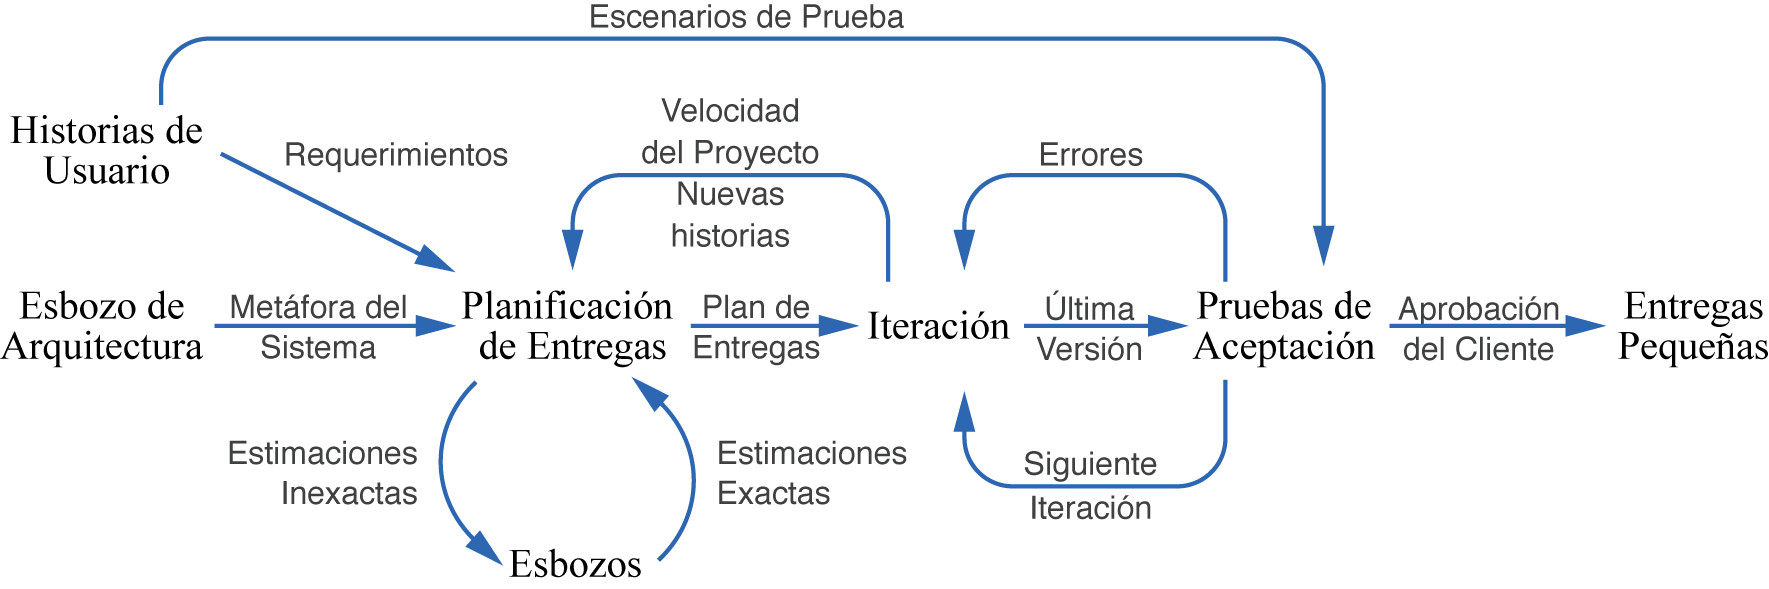
\includegraphics{imagenes/XP-Flujo.png}
	\caption{Flujo de Trabajo en Extreme Programming. \citep{Metodologia_XP_grafico_flujograma_2006}}
	\label{fig:xp_project}
\end{figure}

Una vez realizada la planificación de las entregas se procede al desarrollo iterativo en el cual el cliente selecciona las historias de usuario a desarrollar y los desarrolladores diseñan las \textbf{pruebas} correspondientes. Como resultado de una iteración se obtiene la \textbf{velocidad del proyecto} que a su vez sirve de límite para la selección de las próximas historias a desarrollar. \\

XP recomienda que se realicen \textbf{entregas pequeñas}, de manera continua, de modo que el cliente pueda ofrecer la retroalimentación necesaria.

\subsection{Etapas del Flujo de trabajo en XP}
Xtreme Programming, como lo indica la Figura \ref{fig:xp_project}, contempla varias etapas dentro del flujo de trabajo, las más destacables son:

\begin{enumerate}
	\item \textbf{Historias de usuario:} son similares a los casos de uso, sin embargo no están escritas en un lenguaje técnico dado que es el cliente el encargado de redactarlas, en aproximadamente tres oraciones, basandose en sus necesidades específicas. Deben contener un nivel de detalle razonable de modo que los desarrolladores puedan hacer las estimaciones de tiempo, de manera más acertada, para las entregas. Las historias sirven como fuente de inspiración para la creación de pruebas de aceptación automatizadas \citep{Metodologia_XP_historias2006}.
	
	\item \textbf{Selección de la metáfora del sistema:} a partir de la creación del esbozo de la arquitectura y del conocimiento de las historias de usuario se enmarca el desarrollo del proyecto en una metáfora. La selección de dicha metáfora permite que el equipo de trabajo maneje el mismo criterio, de manera consistente, para los nombres de clases y métodos. Logrando así, que los desarrolladores agilicen la tarea de determinar la existencia de alguna funcionalidad o clase. \citep{Metodologia_XP_metafora2006}

	\item \textbf{Planificación de Entregas:} previo al inicio del desarrollo en iteraciones se lleva a cabo una reunión para crear el plan de entregas. El objetivo de dicha reunión es estimar cada historia del usuario en términos de semanas de programación ideales. Una semana ideal se refiere a cuánto tiempo estima el desarollador que le tomará implementar cada historia y sus pruebas trabajando con dedicación exclusiva al proyecto. Luego de hacer las estimaciones, el cliente procede a seleccionar las historias a implementar de acuerdo a su prioridad \citep{Metodologia_XP_entregas20061} \\ La filosofía para lograr un concenso durante la reunión de planificación de entregas debe girar en torno a cuatro variables: alcance, recursos, tiempo y calidad.
	\begin{itemize}
		\item Alcance: cuánto se tiene por hacer.
		\item Recursos: cuántas personas están disponibles.
		\item Tiempo: cuándo estará listo el proyecto o la entrega.
		\item Calidad: qué tan bueno será el proyecto y que tan bien probado será.
	\end{itemize}
	De estas variables, la gerencia puede seleccionar sólo tres. Los desarrolladores manejarán la última. Por lo general la planificación resultante se mantendrá mientras la velocidad del proyecto sea estable y no surjan nuevas historias de usuario \citep{Metodologia_XP_entregas20062}.

	\item \textbf{Iteración:} una iteración se alimenta de tres fuentes de información: el plan de entregas, la velocidad del proyecto calculada en iteraciones anteriores y los errores reportados en las pruebas de aceptación. El desarrollo de una iteración en XP, contempla en sí varias fases como se describe en la figura \ref{fig:xp_iteration}:
	\begin{figure}[ht]
		\centering
		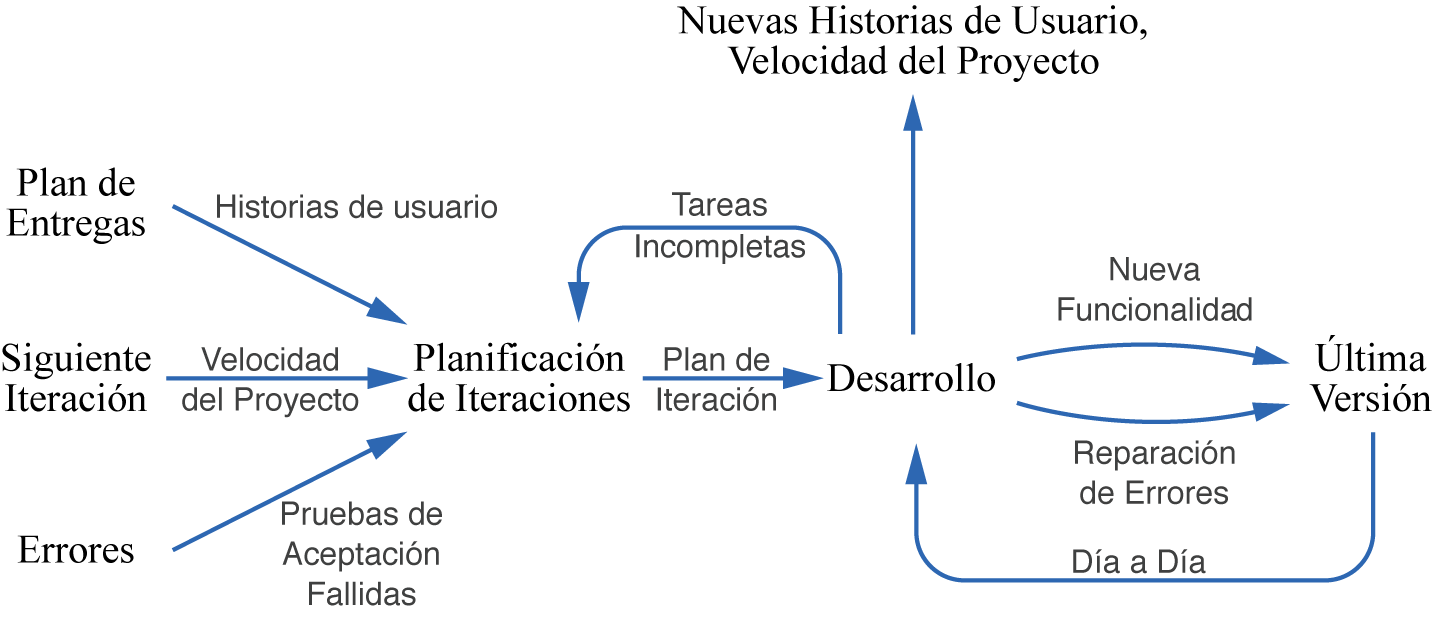
\includegraphics{imagenes/XP-Iteracion.png}
		\caption{Desarrollo iterativo - Iteración. \citep{Metodologia_XP_grafico_it_2006}}
		\label{fig:xp_iteration}
	\end{figure}

	\begin{itemize}
		\item \textbf{Planificación de iteración:} la planificación de cada iteración se realiza al principio de la misma, debe evitarse planificar por anticipado más allá de la iteración en curso, así mismo es importante mantenerse dentro de la planificación y no agregar funcionalidades que no esten planificadas. La estimación de tiempo de cada tarea debe realizarla el desarrollador asignado a dicha tarea; la estimación no debe ser modificada durante la iteración ya que de ello depende lograr mejores estimaciones en las subsiguientes iteraciones, de la misma manera debe respetarse el límite de duración de la iteración en curso \citep{Metodologia_XP_iterativo2006}.
		
		\item \textbf{Desarrollo:} el desarrollo dentro de la iteración describe un día de trabajo bajo la óptica de XP. Al inicio del día se realiza una reunión corta \citep{Metodologia_XP_standup2006} en la que se reportan problemas con sus soluciones y se promueve la concentración en el proyecto. Luego, cada desarrollador, procede a seleccionar una de las tareas asignadas (o una prueba que falle) para desarrollarla en pareja con un compañero. \\
		
		Según \citeauthor{Metodologia_XP_parejas2006}, el \textbf{desarrollo en parejas} es el punto focal del desarrollo, esta metodología promueve un mayor conocimiento del código (funcionalidades y pruebas) por parte de cada miembro del grupo. Esta forma de trabajo está rodeada de cuatro aspectos importantes: \textbf{el intercambio de parejas}  que suele ocurrir cuando alguna pareja requiere ayuda \citep{Metodologia_XP_rotacion2006}, \textbf{integración continua} de nuevo código al proyecto al desarrollar nuevas funcionalidades o pruebas unitarias \citep{Metodologia_XP_integracion2006}, \textbf{reestructuración sin piedad} (refactoring) para simplificar partes complejas del código \citep{Metodologia_XP_refactor2006} y por último \textbf{creación de pruebas unitarias} antes de desarrollar nuevas funcionalidades. \citep{Metodologia_XP_unittest2006}
	\end{itemize}
	
\item \textbf{Velocidad del proyecto}: es un indicador de cuan rápido se está desarrollando el proyecto. Se calcula a partir del número de historias de usuario (o tareas) completadas durante cada iteración. Luego se emplea para determinar cuántas y cuáles historias de usuario (o tareas) serán implementadas durante la reunión de planificación de cada iteración. También es útil cuando se desea determinar cuantas iteraciones serán necesarias para finalizar una entrega mayor \citep{Metodologia_XP_velocidad2006}.

\item \textbf{Pruebas de aceptación o funcionales}
Las pruebas de aceptación son creadas a partir de las ``historias de usuario''. En el transcurso de una iteración las ``historias de usuario'' seleccionadas en la reunión de planificación de la iteración serán traducidas a pruebas de aceptación. El cliente especifica los escenarios en los cuales se probará si una historia de usuario, que puede tener una o varias pruebas, ha sido implementada correctamente.
Las pruebas de aceptación son pruebas de caja negra al sistema, cada una de ellas representa algún resultado esperado del sistema. Los clientes son responsables de verificar la correctitud de la prueba y revisar los resultados de la misma, para así decidir cuál prueba fallida, en caso de que la haya, tiene mayor prioridad. La implementación de una historia de usuario no serán considerada completa mientras no pase todas las pruebas de aceptación asociadas a la historia \citep{Metodologia_XP_testaceptacion2006}.

\end{enumerate}

\subsection{Retroalimentación y Planificación}

La figura \ref{fig:xp_loop} muestra el ciclo donde se indican los tiempos aproximados de planificación, al igual que los tiempos en que se obtiene retroalimentación del trabajo completado.
\begin{figure}[ht]
	 \centering
	 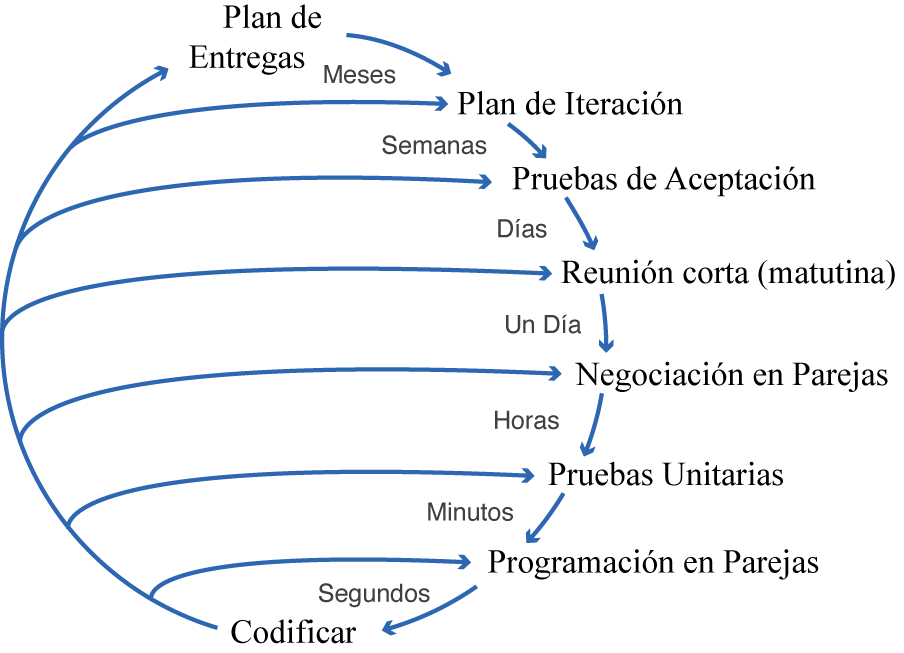
\includegraphics{imagenes/XP-feedback.png}
	 \caption{Ciclo de Planificación y Retroalimentación en Xtreme Programming}
	 \label{fig:xp_loop}
\end{figure}
% -- MVC --
	%!TEX root = ../Libro.tex
\section{Patrón de Arquitectura MVC}
Modelo-Vista-Controlador es un patrón de ingeniería del software que permite crear independencia entre la capa de interfaz, la capa de negocios y la capa de datos, facilitando el modificar la apariencia de la aplicación o las reglas del negocio sin afectar al resto. En el MVC el Modelo representa la información o la data de la aplicación y las reglas del negocio empleadas para manejarla, la Vista corresponde a los elementos de la interfaz del usuario como cuadros de texto, checkbox, etc. y el Controlador maneja los detalles correspondientes a la comunicación con el modelo de la aplicación.

\subsection {Elementos del patrón MVC}

\begin{itemize}
	\item \textbf{Modelo:} representa los datos y las reglas del negocio que manejan el acceso a esos datos. Generalmente el modelo se emplea como una aproximación al proceso original de diseño de la base de datos, por lo que las técnicas de modelado también aplican en la definición del modelo \citep{MVC_Java2002}.
	\item \textbf{Vista:} muestra el contenido del modelo. Accede a los datos del negocio, a través del modelo, y especifica que data debe ser mostrada. Es responsabilidad de la vista el mantener la consistencia en las presentaciones cuando el modelo cambia \citep{MVC_Java2002}.
	\item \textbf{Controlador:} lleva a cabo la traducción de la interacción con la vista a acciones que pueden ser ejecutadas por el modelo. Las acciones realizadas por el modelo incluyen el activar procesos del negocio o cambiar el estado del mismo. En base a la interacción del usuario y la salida de las operaciones del modelo, el controlador responde seleccionando una vista adecuada \citep{MVC_Java2002}.
\end{itemize}

El flujo de control para este patrón es \citep{MVC_WE2007}:
\begin{enumerate}
	\item El usuario interactúa con la interfaz.
	\item El controlador toma el evento de entrada de la interfaz con el usuario.
	\item El controlador notifica al modelo de la acción ejecutada por el usuario, que posiblemente resulta en un cambio en el estado del modelo.
	\item El controlador delega a los objetos de la vista la tarea de desplegar la interfaz de usuario. La vista obtiene sus datos del modelo para generar una interfaz que se adapte a los cambios del mismo. La vista toma los datos del modelo pero este no tiene conocimiento directo sobre la vista.
	\item Se esperan nuevas interacciones en la interfaz de usuario que inicien el ciclo nuevamente.
\end{enumerate}

\subsection {Ventajas}

\begin{itemize}
	\item \textbf{Permite la re-utilización de los componentes del modelo}\\
	La separación entre el modelo y la vista permite emplear varias vistas para un mismo modelo. Como consecuencia de esto los componentes del modelo son más fácil de implementar, probar y mantener, ya que todos los accesos se realizan a través de estos componentes.
	\item \textbf{Mayor facilidad para el soporte de nuevos tipos de clientes}\\
	Sólo es necesario crear nuevas vistas, incorporar alguna lógica en el controlador e integrarlo con la aplicación existente.
	\item \textbf{Facilidad en el diseño}\\
	Las aplicaciones web se han hecho más difíciles de diseñar que las aplicaciones tradicionales, el patrón MVC está siendo usado como una solución a esa dificultad.
\end{itemize}

\subsection {Desventajas}
\begin{itemize}
	\item \textbf{Incrementa la complejidad del diseño}\\
	El patrón introduce algunas clases extras para la separación del modelo, la vista y el controlador.
	\item \textbf{Cierta cohesión entre la vista y el controlador}\\
	Cualquier modificación en la vista suele significar un cambio en el controlador.
\end{itemize}

% 	
% \begin{figure}[ht]
% 	\centering
% 	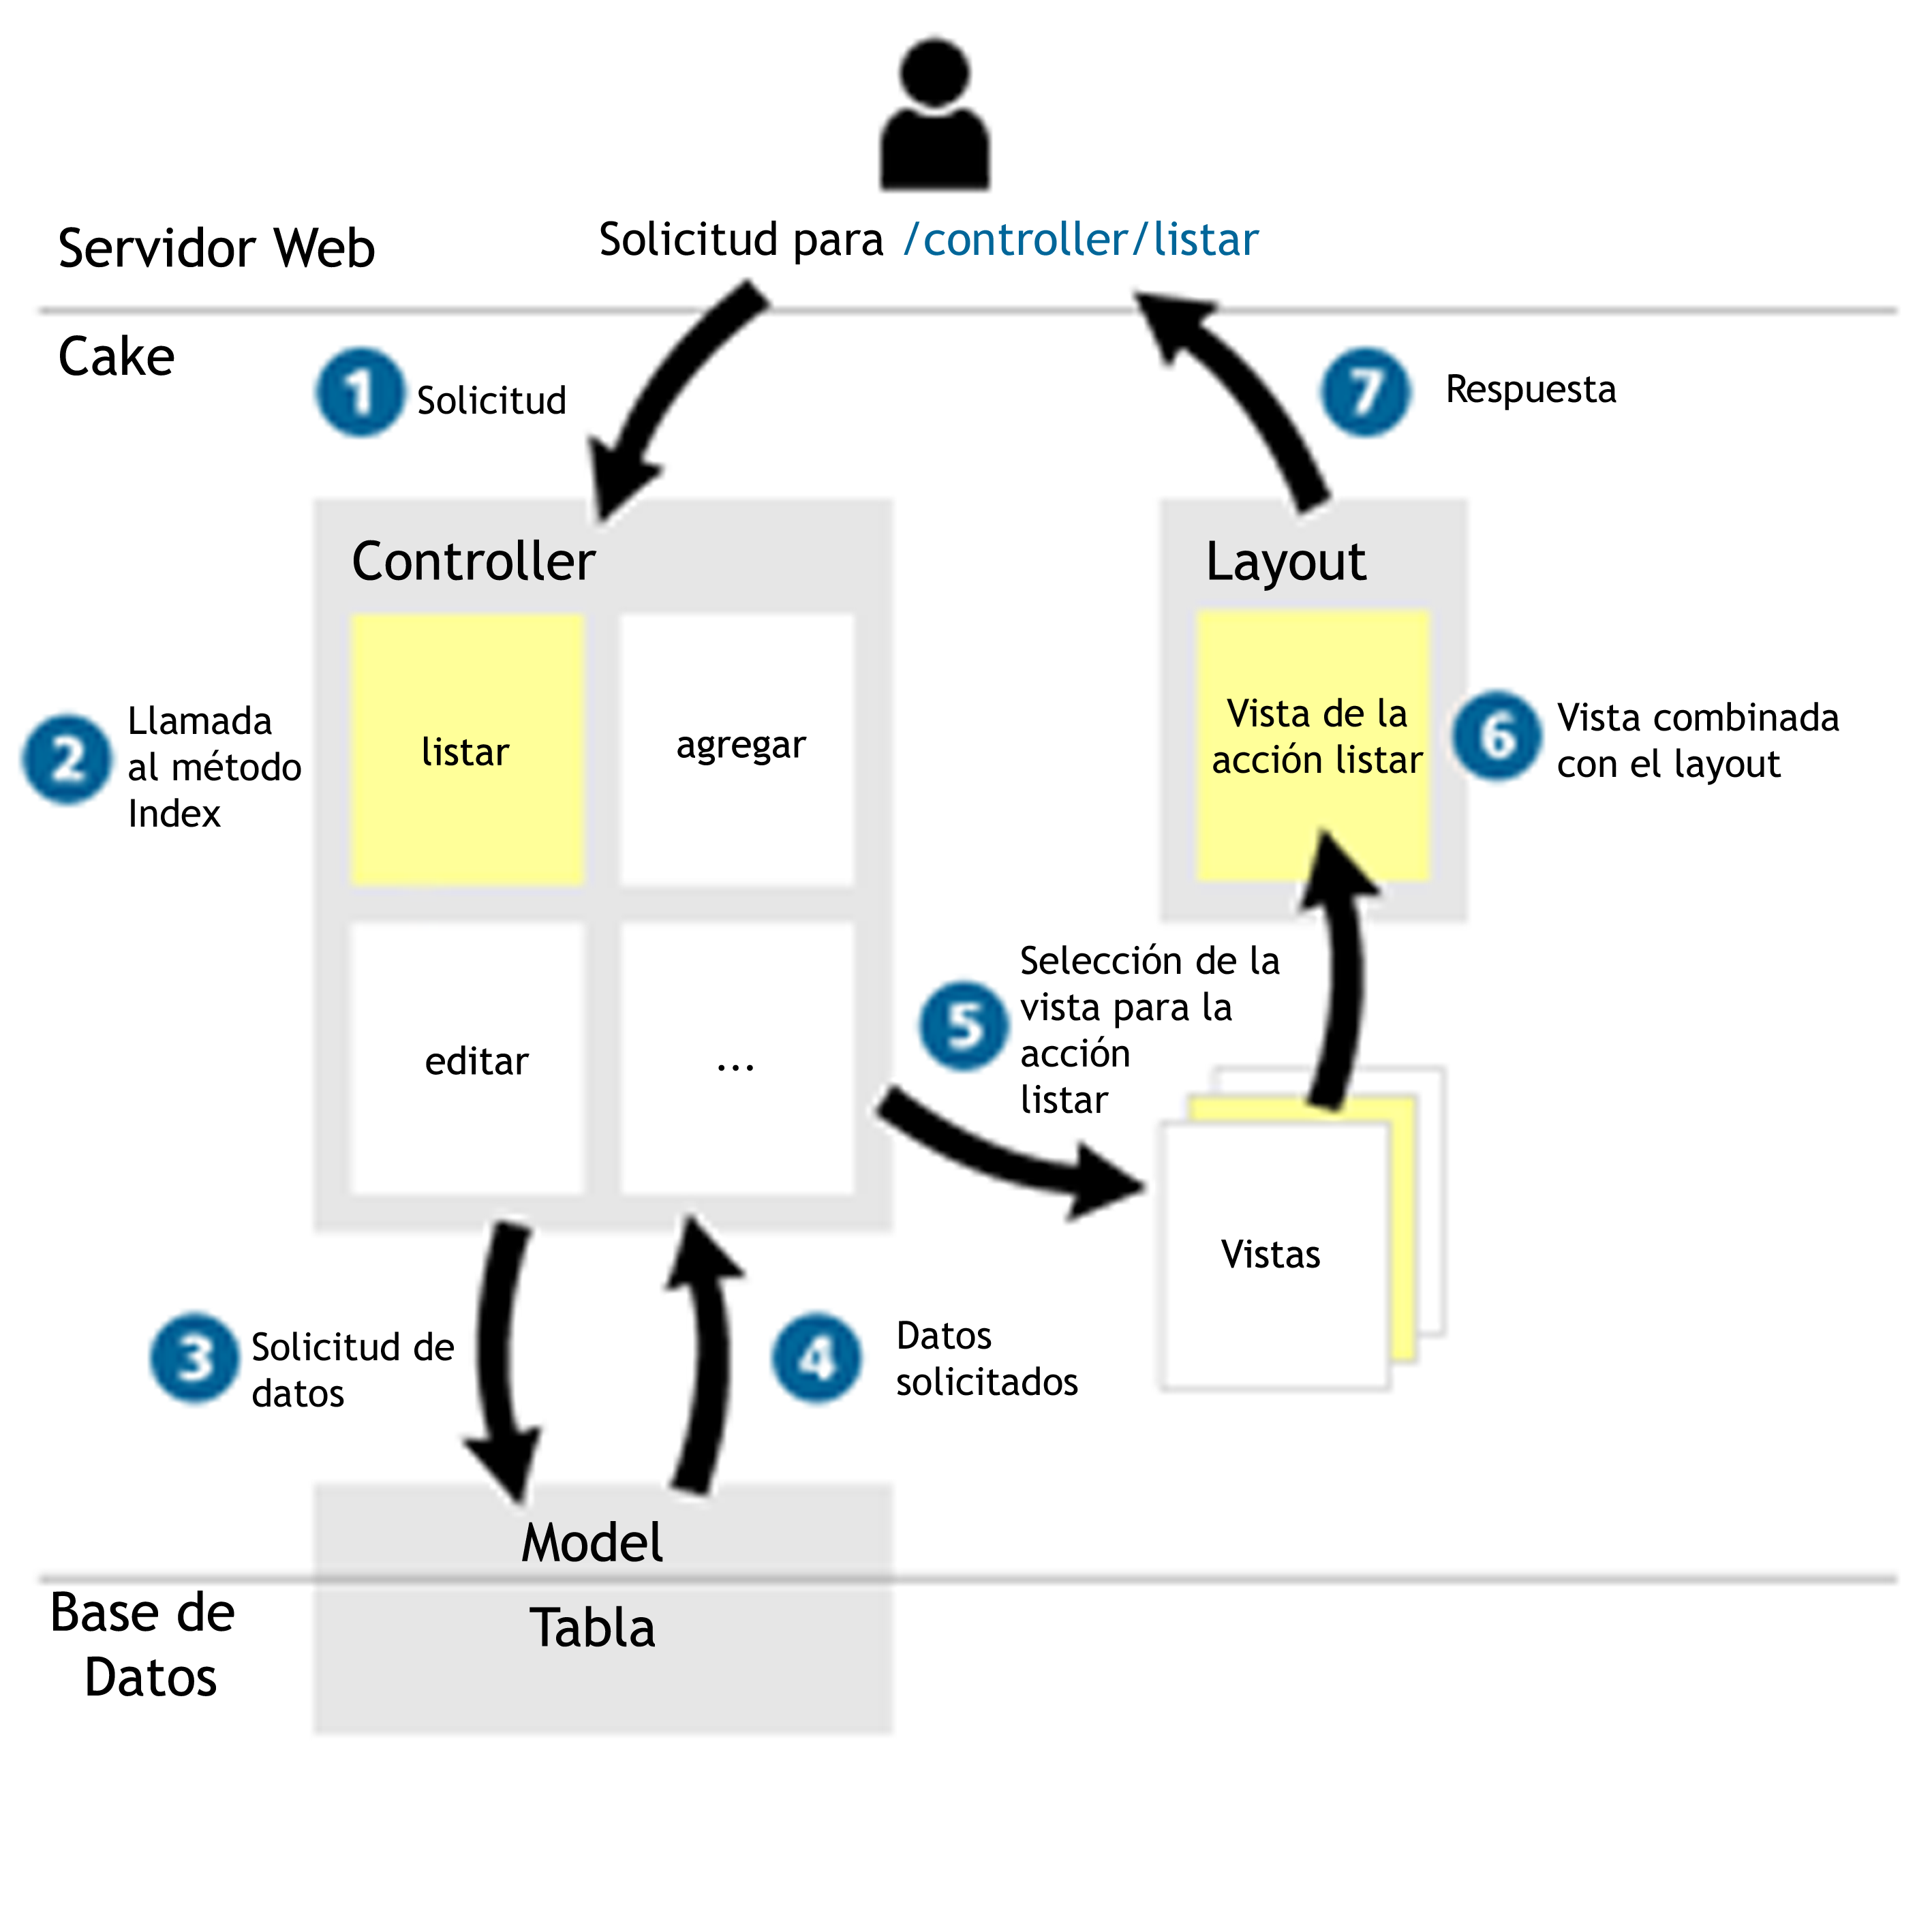
\includegraphics{imagenes/MVC_Cake.png}
% 	\caption{Diagrama del patrón MVC para Cake}
% 	\label{fig:mvc_cake}
% \end{figure}

% -- Metáfora del sistema --
	%!TEX root = ../Libro.tex
\chapter{Diseño}
\section{Metáfora del Sistema}
Siguiendo las indicaciones de la metodología, la metáfora seleccionada para el desarrollo de \textbf{Ósmosis2} es ``el aula de clases tradicional'', en la cual los estudiantes atienden a las clases del profesor. Esto permite que muchas de las herramientas planificadas se integren fácilmente dentro de está metáfora. Por ejemplo las palabras lecciones, foros, conversaciones (chat), encajan sin mucho esfuerzo.

\section{Roles de usuario}
También, dentro de la metáforas, los actores son obvios: estudiante, profesor, ayudante (asistente) y oyente. Esta jerarquía de ``super-roles'' permite asignar a cada usuario su función específica dentro de un curso (un profesor en el curso A puede ser un estudiante en el curso B). Adicional a estos cuatro roles se define uno adicional, el cual no está superditado a un curso en particular, que es el administrador de la plataforma y tiene acceso privilegiado a todas las funciones del sistema.\\

Sin embargo, por lo extenso del proyecto y para agregar mayor semántica dentro de cada herramienta, se han desarrollado ``sub-roles'' que permiten definir las funciones de cada usuario dentro de la herramienta y definir qué super-roles pueden ser asignados dentro de dichos sub-roles.\\

Para conocer sobre las funcionalidades de cada una de las herramientas mencionadas a continuación consultar el \textbf{Apéndice B}, en el cual se describen las características del sistema en función de las herramientas y recursos que lo conforman.

\subsubsection{Foro}
\begin{itemize}
	\item \emph{Moderador}: el moderador de un foro es el encargado de mantener las conversaciones dentro de un ambiente de respeto y cerrar las conversaciones cuando lo considere pertinente.\\
		\textbf{Super-Roles:} instructor y ayudante.
	\item \emph{Forista}: es la persona que escribe sus comentarios, sobre un tema específico, en el foro.\\
		\textbf{Super-Roles:} estudiante. 
\end{itemize}

\subsubsection{Blog}
\begin{itemize}
	\item \emph{Escritor}: el escritor de un blog es aquella persona que plasma ideas o comentarios en él para compartirlos con el resto de la comunidad.\\
		\textbf{Super-Roles:} instructor, ayudante y estudiante.
	\item \emph{Lector}: es el lector de los comentarios del blog de otra persona.\\
		\textbf{Super-Roles:} instructor, ayudante, estudiante y visitante.
\end{itemize}

\subsubsection{Wiki}
\begin{itemize}
	\item \emph{Supervisor}: es el encargado de supervisar la calidad de información colocada en el wiki, que sea adecuada.\\
		\textbf{Super-Roles:} instructor.
	\item \emph{Editor}: son aquellas personas que participan en el wiki agregando información relacionada a los temas de los cursos o que considere de interés para otros estudiantes o instructores.\\
		\textbf{Super-Roles:} ayudante y estudiante.
	\item \emph{Lector}: es el lector de la información contenida en el wiki. Puede ver el historial o comparar versiones del contenido allí escrito.\\
		\textbf{Super-Roles:} visitante.
\end{itemize}

\subsubsection{Chat}
\begin{itemize}
	\item \emph{Moderador}: al igual que en el foro, el moderador de un chat es el encargado de mantener las conversaciones dentro de un ambiente de respeto, así mismo puede amonestar a un participante si lo considera necesario.\\
		\textbf{Super-Roles:}instructor y ayudante.	
	\item \emph{Participante}: son las personas que participan en conversaciones sobre distintos temas empleando el chat como medio para intercambiar ideas en tiempo real.\\
		\textbf{Super-Roles:} estudiante.
\end{itemize}

\subsubsection{Mensajería}
\begin{itemize}
	\item \emph{Remitente}: es la persona que envía un mensaje (e-mail) a una o más personas.\\
		\textbf{Super-Roles:} instructor, ayudante y estudiante.
	\item \emph{Destinatario}: es la persona que recibe un mensaje. Puede realizar las opciones típicas de un servicio de mensajería (leer el mensaje, eliminarlo, ver la bandeja de entrada, etc.).\\
		\textbf{Super-Roles:} instructor, ayudante y estudiante.
\end{itemize}

\subsubsection{Evaluaciones}
\begin{itemize}
	\item \emph{Evaluador}: es la persona que crea, aplica y corrige las evaluaciones o actividades asignadas a un grupo de personas.\\
		\textbf{Super-Roles:} instructor y ayudante.
	\item \emph{Evaluado}: es la persona que responde una evaluación aplicada por el evaluador.\\
		\textbf{Super-Roles:} estudiante.
\end{itemize}

\subsubsection{Agenda}
\begin{itemize}
	\item \emph{Planificador}: es la persona que planifica y agrega un nuevo evento a la agenda.\\
		\textbf{Super-Roles:} instructor y ayudante.
	\item \emph{Lector}: es la persona que observa los eventos plasmados en la agenda.\\
		\textbf{Super-Roles:} instructor, ayudante, estudiante y oyente.
\end{itemize}

\subsubsection{Lecciones}
\begin{itemize}
	\item \emph{Tutor}: es la persona que proporciona o dicta la lección\\
			\textbf{Super-Roles:} instructor y ayudante.
	\item \emph{Aprendiz}: es aquel que utiliza la información contenida en la lección.\\
			\textbf{Super-Roles:} estudiante.
\end{itemize}

\subsubsection{Casillero}
\begin{itemize}
	\item \emph{Propietario}: es aquella persona que es dueña del casillero\\ \textbf{Super-Roles:} instructor, ayudante y estudiante.
	\item \emph{Lectores}: son las personas que pueden visualizar archivos almacenados en los casilleros de otros usuarios\\ \textbf{Super-Roles:} instructor, ayudante, estudiante y oyente.
\end{itemize}

\subsubsection{Portafolio}
\begin{itemize}
	\item \emph{Dueño}: el dueño del portafolio es el único que tiene capacidad de modificarlo y decidir qué usuarios pueden acceder a él.\\
		\textbf{Super-Roles:} instructor, ayudante y estudiante.
\end{itemize}
	%!TEX root = ../Libro.tex
\section{Historias de Usuario}
A continuación se presentan, organizadas por herramienta, las historias de usuario según redactadas según las recomendaciones de la metodología XP.

\subsubsection{Manejo de Usuarios}
\begin{itemize}
	\item \textbf{Registrar usuario individuales y por lotes}\\
	El administrador tiene la opción de registrar a los usuarios del sistema de forma individual o por grupos (registrar a todos los estudiantes del curso). De igual manera, cada estudiante puede registrarse por su cuenta y de forma individual.
	\item \textbf{Iniciar sesión}\\
	El usuario ya registrado, introduce el login y el password para tener acceso al sistema y sus funcionalidades.
	\item \textbf{Cerrar sesión}\\
	El usuario cierra la sesión a través de la cual ha estado trabajando y abandona el sistema.
	\item \textbf{Manejo de permisos}\\
	El sistema debe permitir asignar roles a los usuarios con respecto a toda la plataforma (administrador,miembro,visitante) y dentro de cada curso (profesor, estudiante,asistente).
	\item \textbf{Eliminar usuario}\\
	Se pueden eliminar los usuarios del sistema de forma individual o por grupos de modo que sus datos no sean válidos para acceder al sistema, sin embargo debe ser posible conservar toda la información generada por este. Esta eliminación debe poder realizarse en lotes.
\end{itemize}

\subsubsection{Foros}
\begin{itemize}
	\item \textbf{Crear tema}\\
	Los profesores del curso tienen la potestad de crear temas para delimitar las discusiones del foro.
	\item \textbf{Iniciar discusión}\\
	Cualquier miembro del curso puede iniciar una discusión dentro de cualquiera de los temas existentes del foro.
	\item \textbf{Responder hilo de discusión}\\
	Los usuarios pueden responder en las discusiones iniciadas en el foro.
	\item \textbf{Editar mensaje}\\
	Cualquier mensaje en los hilos de discusión deben ser modificables por sus respectivos dueños.
	\item \textbf{Puntuar un comentario}\\
	Los usuarios del foro, podrán asignar una evaluación de la calidad de los mensajes de sus compañeros.
	\item \textbf{Programar fecha de cierre}\\
	El sistema permite cerrar un tema o una discusión de modo que ningún participante pueda agregar nuevos mensajes. Este cierre puede ser programado de modo que se ejecute automáticamente llegada la fecha.
\end{itemize}

\subsubsection{Intercambio de Archivos}
\begin{itemize}
	\item \textbf{Subir archivo}\\
	El sistema debe permitir a los usuarios subir archivos al sistema, estos archivos serán de acceso público.
	\item \textbf{Modificar datos del archivo}\\
	Los usuarios pueden modificar los datos (título o descripción) del archivo que subió al sistema.
	\item \textbf{Ordenar casillero}\\
	El usuario del casillero debe poder organizar sus archivos como lo desee, creando carpetas y moviendo archivos de lugar.
	\item \textbf{Acceso al casillero}\\
	Todo casillero será accesible públicamente y existirá una carpeta especial para hacer entregas en la que todo usuario podrá dejar archivos que sólo el dueño del casillero podrá ver.
	\item \textbf{Manejar versiones para archivos}\\
	El sistema permite manejar la actualización de versiones de los archivos subidos. Esto facilita el control de los posibles cambios que pueda sufrir un archivo.
	\item \textbf{Detección de virus}\\
	El sistema debe suministrar un antivirus que verifique que los archivos a subir o descargar no posean virus que puedan afectar a los usuarios.
\end{itemize}

\subsubsection{Mensajería Interna}
\begin{itemize}
	\item \textbf{Enviar mensaje}\\
	Los usuarios pueden enviar mensajes a otros usuarios del sistema. Los mensajes pueden ser leídos dentro del sistema o pueden ser redirigidos al correo electrónico del usuario.
	\item \textbf{Leer mensaje}\\
	El sistema permitirá a los usuarios leer los mensajes que ha recibido
 	\item \textbf{Manejar libreta de direcciones}
	\begin{itemize}
		\item \textbf{Agregar contactos}\\
		Los usuarios poseen una ``libreta'' en la cual pueden almacenar los datos de contacto de otros usuarios del sistema. El sistema permite agregar nuevos contactos con la información de cada uno de ellos.
		\item \textbf{Buscar contacto}\\
		El usuario que posee contactos en su libreta puede realizar una búsqueda de los datos de una persona en particular, ingresando el nombre del contacto a buscar o cualquier otra información relevante.
		\item \textbf{Eliminar contacto}\\
		El usuario que posee una libreta de contactos puede eliminar un contacto y toda la información del mismo.
		\item \textbf{Editar información de contacto}\\
		El usuario puede agregar datos adicionales sobre sus contactos.
		\item \textbf{Exportar contactos}\\
		El sistema permite que los usuarios exporten su lista de contactos a otros formatos digitales que faciliten la impresión o manejo de los mismos fuera del sistema.
	\end{itemize}
\end{itemize}

\subsubsection{Blog}
\begin{itemize}
	\item \textbf{Entradas}\\
	El escritor del blog debe se capaz de escribir y modificar las entradas de su blog.
	\item \textbf{Eliminar entrada}\\
	El escritor del blog puede, en cualquier momento, eliminar una entrada de su blog.
	\item \textbf{Listar entradas}\\
	Se pueden visualizar las entradas registradas en el blog. La cantidad de información mostrada dependerá de las configuraciones seleccionadas por el dueño del blog.
	\item \textbf{Agregar comentario}\\
	Dependiendo de las configuraciones definidas por el escritor del blog, los lectores podrán dejar comentarios en las entradas publicadas.
	\item \textbf{Enviar trackback/pingback}\\
	El sistema de blogs debería permitir manejar trackbacks y pingbacks para permitir la comunicación con otros blogs dentro y fuera del sistema.
	\item \textbf{Recibir trackback/pingback}\\
	Al recibir una petición de trackback o pingbak se debe registrar un comentario en la entrada correspondiente que exprese que ha sido realizada esta acción
	\item \textbf{Importar blog externo}\\
	El usuario registrado, escritor de un blog externo, tiene la capacidad de indicarle al sistema donde se aloja dicho blog de manera que tome de ahí las nuevas entradas. 
\end{itemize}

\subsubsection{Wiki}
\begin{itemize}
	\item \textbf{Crear página}\\
	Los miembros del curso pueden crear y modificar páginas en el wiki.
	\item \textbf{Historia de Modificaciones}\\
	El sistema debe llevar un registro de los cambios que se realizan en cada página de cada wiki. 
	\item \textbf{Restaurar página}\\
	En cualquier momento el usuario podrá restaurar una página del wiki a una versión anterior.
	\item \textbf{Comparar versiones de páginas}\\
	El usuario podrá comparar distintas versiones de una página para detectar los cambios realizados. Debe ser posible saber el autor de los cambios.
	\item \textbf{Manejo de borradores}\\
	El usuario tendrá la posibilidad de almacenar borradores de las páginas que está modificando.
	\item \textbf{Manejo de discusiones}\\
	Cada página debe permitir una sección para que los usuarios discutan los contenidos de dicha página.
\end{itemize}

\subsubsection{Chat}
\begin{itemize}
	\item \textbf{Ver historial de conversaciones}\\
	El sistema debe permitir al moderador del curso ver los registros (historial) de las conversaciones.
	\item \textbf{Expulsar usuario}\\
	El moderador de la sala de chat puede expulsar a un participante de manera temporal o permanente.
	\item \textbf{Registrar pregunta desde el chat}\\
	Los participantes tienen la posibilidad de copiar preguntas hechas en el chat (con sus respuestas) a una sección permanente de preguntas importantes.
\end{itemize}

\subsubsection{Pizarra}
El instructor o el ayudante pueden configurar una sesión de trabajo en la ``pizarra''. En ella podrá mostrar material multimedia (PDF, presentaciones, dibujos y videos) o escrita (chat y pizarra).

\subsubsection{Lecciones}
\begin{itemize}
	\item \textbf{Crear lección}\\
	El profesor del curso puede subir al curso una lección en formato SCORM.
 	\item \textbf{Ver lección}
	El sistema debe proveer un visor de lecciones SCORM de modo que los miembros del curso puedan revisarla en línea.
\end{itemize}

\subsubsection{Enlaces}
\begin{itemize}
	\item \textbf{Agregar enlace}\\
	Cada curso debe tener una sección de enlaces a recursos de interés. Cada miembro que lo desee podrá agregar recursos por esta vía.
	\item \textbf{Modificar enlace}\\
	Cada miembro podrá modificar o eliminar los enlaces que haya agregado.
\end{itemize}

\subsubsection{Calendario/Agenda}
Los miembros del curso podrán registrar, modificar y eliminar eventos de la agenda. Dichos eventos serán visibles por el curso.\\

\subsubsection{Trabajo desconectado}
\begin{itemize}
	\item \textbf{Agregar Podcast/Screencast}\\
	El blog debe soportar podcasting y screencasting.
	\item \textbf{Descargar contenidos del curso}\\
	El usuario puede descargar el material del curso para usarlo posteriormente sin necesidad de estar conectado con el sistema.
\end{itemize}

\subsubsection{Agregador de Noticias}
Cada curso podrá agregar de manera automática noticias generadas en otras páginas.

\subsubsection{Grupos de Trabajo}
\begin{itemize}
	\item \textbf{Crear grupo}\\
	El profesor o ayudante puede crear grupos de trabajo con los estudiantes del curso.
	\item \textbf{Modificar grupo}\\
	El profesor o ayudante de un curso podrá modificar cualquier grupo de trabajo para agregar o eliminar un miembro del grupo.
	\item \textbf{Eliminar grupo}\\
	El profesor o ayudante podrá eliminar un grupo una vez finalizada la actividad para la cual fue creado.
\end{itemize}

\subsubsection{Comunidad}
\begin{itemize}
	\item \textbf{Listar cursos}\\
	El sistema debe exponer a la comunidad todos los cursos disponibles en la plataforma.
	\item \textbf{Listar entradas de blogs}\\
	El sistema debe exponer las entradas de los blogs.
	\item \textbf{Notificaciones Globales}\\
	El sistema debe permitir a los administradores colocar notificaciones globales para todos los usuarios.
	\item \textbf{Mostrar noticias externas}\\
	El sistema debe permitir a los administradores seleccionar una o más fuentes de noticias que se mostrarán como notificaciones globales.
\end{itemize}

\subsubsection{Portafolios}
\begin{itemize}
	\item \textbf{Crear perfil}\\
	El usuario registrado (instructor, ayudante o estudiante) puede crear un perfil con sus datos personales e información correspondiente a los estudios cursados, entre otros. Podrá crear un currículo virtual del cual será dueño. 
	\item \textbf{Configurar perfil}\\
	El dueño del portafolio podrá editar la información suministrada al crear su perfil inicial para modificar o eliminar datos.
	\item \textbf{Ver perfil}\\
	Los usuarios registrados y los visitantes pueden visualizar los datos del perfil de otro usuario o de ellos mismos. La cantidad de información suministrada dependerá del nivel de permisos que tenga el usuario que visualiza el perfil.
	\item \textbf{Configurar portafolios}\\
	El dueño del portafolios podrá seleccionar los elementos que desea mostrar públicamente, el portafolio completo estará disponible para que lo envíe personalmente a quienes desee mostrar la información completa.
	\item \textbf{Editar portafolios}\\
	El dueño del portafolio puede agregar información nueva, así como eliminar o modificar la información existente.  
	\item \textbf{Exportar portafolios}\\
	El dueño del portafolio podrá exportar su perfil personal con el estilo de un currículo, indicando la información que desea mostrar y cómo desea presentarla.
\end{itemize}

\subsubsection{Pruebas en línea}
\begin{itemize}
	\item \textbf{Crear preguntas}\\
	El instructor o el ayudante pueden elaborar preguntas que, posteriormente, les permitan crear una prueba o utilizarlas en otra actividad 
	\item \textbf{Modificar preguntas}\\
	El instructor o el ayudante pueden editar las preguntas creadas para cambiar su contenido o adaptarla a algún tipo de actividad. Debe tenerse en cuenta que dichas preguntas pueden haber sido usadas en otras pruebas.
	\item \textbf{Crear pruebas}\\
	El instructor o el ayudante pueden elaborar pruebas para evaluar el contenido de la materia del curso. Estas pruebas tendrán asociadas una puntaje.
	\item \textbf{Modificar pruebas}\\
	El instructor o el ayudante pueden modificar las pruebas creadas. Se podrá agregar una pregunta, eliminarla o cambiar su puntaje.
	\item \textbf{Guardar pruebas}\\
	El instructor o el ayudante pueden guardar las pruebas elaboradas para reutilizarlas en futuros cursos.
	\item \textbf{Evaluar pruebas}\\
	El instructor o el ayudante pueden corregir las preguntas de las pruebas aplicadas a los estudiantes y asignarles el puntaje obtenido. Posteriormente este puntaje se vera reflejado en el acta de calificaciones. 
\end{itemize}

\subsubsection{Actividades Evaluadas}
El profesor o ayudante podrá asignar una actividad, con una puntuación definida, a los estudiantes.

\subsubsection{Control de calificaciones}
\begin{itemize}
	\item \textbf{Crear tabla de control de evaluación}\\
	El instructor podrá crear una tabla de calificaciones en la cual se plasmara las notas obtenidas por los estudiantes tanto en las actividades evaluadas como en las pruebas, luego se podrá totalizar el puntaje para cada estudiante del curso. 
	\item \textbf{Modificar tabla de control de evaluación}\\
	El instructor podrá editar la tabla de calificaciones para agregar nuevas actividades o pruebas a evaluar, para cambiar el puntaje de las ya existentes o para eliminarlas. 
	\item \textbf{Exportar tabla de calificaciones}\\
	El sistema permitirá al instructor generar un acta de las calificaciones del curso con las actividades realizadas y el puntaje obtenido por los estudiantes en cada una de ellas.
\end{itemize}

\subsubsection{Manejo del Curso}
\begin{itemize}
	\item \textbf{Crear curso}\\
	El instructor podrá crear un curso que corresponderá a la materia a dictar. Podrá dar la descripción del mismo, los horarios, etc. y agregar a los estudiantes que lo tomarán. Adicionalmente podrá agregar a la plantilla del curso aquellas herramientas, disponibles en el sistema, que se consideren adecuadas para lograr los objetivos del mismo.
	\item \textbf{Programar aparición de recursos}\\
	EL sistema debe permitir a los profesores definir las fechas en las que algún contenido estará disponible para que los estudiantes lo utilicen.
	\item \textbf{Guardar estructura de un curso}\\
	El sistema debe permitir que la estructura de un curso pueda ser guardada para ser utilizada como plantilla de otro curso.
\end{itemize}

\subsubsection{Seguimiento de usuarios}
\begin{itemize}
	\item \textbf{Listar usuarios en línea}\\
	Los miembros podrán en cualquier momento conocer qué compañeros se encuentran usando la plataforma.
	\item \textbf{Ver historial de navegación}
	El profesor tendrá una sección en la que podrá observar el uso que le dan los estudiantes al plataforma, de modo que pueda detectar a los estudiantes poco participativos o con problemas.
\end{itemize}

\subsubsection{Manejo de estadísticas}
El sistema debe extraer, a partir de los datos recabados en el seguimiento de los usuarios, datos de interés estadístico sobre el uso de los recursos y herramientas. Estos datos deben ser visibles para profesores y administradores.

\subsubsection{Learning Objects}
La plataforma debe permitir a los usuarios generar Learning Objects a partir de los recursos disponibles.
	%!TEX root = ../Libro.tex
\section{Requerimientos no-funcionales}
Las siguientes características y condiciones técnicas que deben cumplirse en Ósmosis2:

\subsection{Capacidad de mantenimiento}
Esta característica engloba los requerimientos relacionados con la sustentabilidad y capacidad de crecimiento que debe tener el sistema en el tiempo. Ósmosis2 debe cumplir con:
\begin{enumerate}
	\item \textbf{Modularidad}\\
	El código fuente del sistema debe contar con una separación clara de sus capas utilizando la arquitectura MVC, de modo que el crecimiento de la aplicación sea organizado.
	\item \textbf{Plug-and-play} \\
	La arquitectura del sistema debe ser de tal manera que cada herramienta se conecte y esté lista para usar. De la misma manera, debe ser igual de fácil desactivar las herramientas.
	\item \textbf{Documentación clara}\\
	El sistema debe contar con una documentación del código clara y completa. Adicionalmente, el sistema debe contar con manuales de uso para desarollador y usuario.
\end{enumerate}

\subsection{Usabilidad y Accesibilidad}
El sistema debe respetar las pautas definidas por la W3C para la accesibilidad en el desarrollo web así como los principios básicos del diseño universal. Debe contar con una interfaz gráfica intuitiva y fácil de usar compatible con cualquiera de los navegadores web de mayor uso (Firefox 2, Internet Explorer 6, Opera 9, Safari 3 y posteriores).

\subsection{Prestaciones}
En esta característica se definen las condiciones que deberá soportar la aplicación a nivel de:
\begin{enumerate}
	\item \textbf{Escalabilidad} \\
	Es un aspecto de gran importancia ya que la plataforma debe manejar, desde sus primeras versiones, miles de usuarios, cantidad que se espera aumentará progresivamente con la incorporación de nuevas instituciones educativas a la plataforma. Así mismo debe permitir el crecimiento rápido en los servicios, de modo que se pueda dar respuesta rápida a los nuevos requerimientos que puedan surgir.
	\item \textbf{Rendimiento} \\
	El sistema debe ejecutar las operaciones de manera eficiente, para ello debe manejar aspectos como la concurrencia y caching de resultados, de modo que sea posible manejar grandes cantidades de peticiones.
\end{enumerate}

\subsection{Seguridad}
\begin{enumerate}
	\item \textbf{Autenticación} \\
	El acceso al sistema debe estar restringido por el uso de claves asignadas a cada uno de los usuarios.
	\item \textbf{Listas de acceso} \\
	El sistema debe permitir que los usuarios tengan acceso para la modificación de sólo los recursos que su rol les permita. Dicho roles deben definirse en función de cada curso.
	\item \textbf{Trazabilidad} \\
	El sistema deberá contar con mecanismos que permitan el registro de las actividades realizadas por cada usuario.
	\item \textbf{Confidencialidad} \\
	El sistema debe permitir que cada usuario determine qué información desea revelar dentro de la aplicación.
\end{enumerate}

% -- Marco Tecnológico --
	%!TEX root = ../Libro.tex
\chapter{Marco Tecnológico}
Este capítulo tiene como principal finalidad presentar las opciones que fueron consideradas para el entorno (lenguaje-framework) que se utilizaría para el desarrollo de Ósmosis2; comparando dichas opciones en diferentes aspectos.
Posteriormente se presenta la opción seleccionada y se justifica dicha selección en función de los requerimientos específicos de la aplicación y de otras variables importantes.

\section{Entorno de desarrollo}
Para el desarrollo de Ósmosis2 se buscó un entorno que permitiese solucionar uno de los problemas presentes en la plataforma actual: propiciar la escalabilidad sin sacrificar la facilidad y la velocidad de desarrollo.\\

Para asegurar la escalabilidad era necesario considerar lenguajes de programación que hubiesen demostrado con anterioridad su confiabilidad. Para cumplir con el requerimiento de facilidad en el desarrollo es necesario seleccionar algún framework que ofrezca al desarrollador un entorno en el que hayan elementos pre-construidos de manera que sólo deba ensamblar, de manera ordenada y estructurada, las partes para lograr la tarea que desea.\\

Bajo estos requisitos iniciales, la decisión debía ser un balance entre estabilidad del lenguaje (en su historia y a futuro) y la facilidad que ofrece el framework estudiado. La selección inicial de lenguajes se basó en el nivel de conocimientos de los desarrolladores, por ello se consideraron \textbf{JSP} por su robustez, \textbf{PHP} por su larga historia soportando exitosamente a muchas aplicaciones web y \textbf{Ruby} por el reciente éxito (publicitario) que ha tenido.\\ 

Una vez seleccionados los lenguajes, se consideró un solo framework para cada uno:
\begin{itemize}
\item \textbf{JSP}: Struts
\item \textbf{Ruby}: Rails
\item \textbf{PHP}: CakePHP
\end{itemize}

\subsection{JSP/Struts}
Struts es un framework de código abierto para la construcción de aplicaciones web basadas en Servlets/JSP bajo el paradigma MVC. Su principal característica es que su implementación de MVC tiene como punto medio al controlador que es el que conecta al modelo con la vista. Sin embargo, Struts no ofrece una capa de acceso a datos sino que recomienda algunas como Hibernate, EJB, Cayenne, etc. Situaciones parecidas se presentan en las capas de vista y de lógica del negocio (incluso la validación de datos), en las cuales se deben conectar otros frameworks especializados \citep{Struts_2008}. \\

En este sentido Struts es altamente flexible, pero dicha flexibilidad suele generar confusión entre los desarrolladores. Uno de los principales problemas que presenta Struts es que frena la velocidad de desarrollo al requerir archivos de configuración en formato XML que debe ser modificado cada vez que se desea implementar una nueva funcionalidad. Muchos defensores de Struts apelan a que dichas configuraciones no son necesario tocarlas si se hace uso de las herramientas automatizadas que ofrecen los IDEs (Integrated Development Enviroment). Sin embargo bajo los requerimientos de Ósmosis, esto se traduce en otra razón en contra. \\

El gran elemento a favor de Struts es la robustez que ofrece un lenguaje orientado a objetos y las muchas librerías existentes que se pueden usar. Sin embargo, en este proyecto tan importante como la reutilización de librerías, es la facilidad y rapidez en el desarrollo de nuevas funcionalidades.

\subsection{Ruby/Rails}
Rails es un framework MVC completo para el desarrollo de aplicaciones web sobre bases de datos. Por completo se entiende que es un framework que ofrece las funcionalidades necesarias para manejar todos los niveles de una aplicación: acceso a datos, validación y reglas del negocio, etc.\\

Rails favorece la convención sobre la configuración, lo cual disminuye la cantidad de detalles que son necesarios recordar en comparación con Struts. Adicionalmente ofrece al desarrollador herramientas para minimizar la cantidad de código necesario, potenciando la reutilización de código. Rails al ser completo, ofrece soporte para validación y abstracción de la base de datos. \\

El rendimiento es uno de los principales problemas de Rails, un ejemplo de este tipo de problemas se presentó con el servicio web Twitter en el cual millones de usuario envían mensajes constantemente lo cual significó constantes caídas del servicio.

\subsection{PHP/CakePHP}
PHP es el lenguaje de mayor uso y presencia en la web, en la actualidad. Es un lenguaje interpretado que, al igual que Ruby, no es fuertemente tipado.\\

PHP tiene una larga trayectoria en el desarrollo web, con corporaciones como Yahoo! usándolo para potenciar sus sitios. Tal vez unos de los más grandes problemas que han sido destacados por los detractores de PHP son las vulnerabilidades detectadas en muchas aplicaciones como resultado de malas prácticas potenciadas por el lenguaje, sin embargo frameworks de desarrollo como Cake se han encargan de cerrar dichos agujeros.\\

CakePHP es un framework que toma muchos de los conceptos útiles de Rails. Es también un framework completo que ofrece código útil para el desarrollo de las interfaces hasta la abstracción del acceso a la base de datos y, como Rails, se basa en la convención sobre la configuración.\\

Según \citeauthor{Heinemeier_2008}, una de las ventajas de CakePHP sobre Rails es el lenguaje sobre el cual se contruye: para PHP está probado que escala bien. Sin embargo, su queja contra PHP se reduce a lo desordenado que puede llegara a ser el código de este lenguaje. \citep{Heinemeier_2008}. Pero, por otra parte, este es uno de los problemas que CakePHP viene a solucionar.

\subsection{Sinopsis y selección}
El cuadro \ref{tab:evaluacion_entorno} resume los puntos destacados anteriormente junto con otros aspectos considerados para la decisión. \\

\begin{table}[h]
\centering  
\begin{tabular}{lccc} \hline
	\multicolumn{1}{c}{\multirow{2}{*}{\textbf{Criterios}}} & \multicolumn{3}{c}{\textbf{Entornos de desarrollo}} \\ \cline{2-4}
	\multicolumn{1}{c}{} & \textbf{JSP/Struts} & \textbf{Ruby/Rails} & \multicolumn{1}{c}{\textbf{PHP/CakePHP}} \\ \hline \hline \\[-0.3cm]
	
	\textbf{Validación de datos}		& X & X & X \\[0.3cm]
	\textbf{Framework completo}			& - & X & X \\[0.3cm]
	\textbf{Agilidad de desarrollo}		& - & X & X \\[0.3cm]
	\textbf{Soporte de la comunidad}	& X & X & X \\[0.3cm]
	\textbf{Documentación}				& X & X & - \\[0.3cm]
	
	\multicolumn{4}{>{\columncolor[rgb]{0.9,0.9,0.9}}c}{\textbf{Requerimientos no funcionales}} \\ \\[-0.3cm]
	\textbf{Módulos Plug-and-Play}						& - & X & X \\[0.3cm]
	\textbf{Encriptación y Autenticación automatizada}	& - & X & X \\[0.3cm]
	\textbf{Listas de acceso}							& - & X & X \\[0.3cm]
	\textbf{Escalabilidad y Rendimiento}				& X & - & X \\[0.3cm]
	
	\multicolumn{4}{>{\columncolor[rgb]{0.9,0.9,0.9}}c}{\textbf{Otros aspectos}} \\ \\[-0.3cm]
	\textbf{Dominio del lenguaje y framework}	& X & - & X \\[0.3cm] \hline
	
	\multicolumn{1}{>{\columncolor[rgb]{0.9,0.9,0.9}}l}{\textbf{Total}} &
		\multicolumn{1}{>{\columncolor[rgb]{0.9,0.9,0.9}}c}{\texttt{\textbf{5/10}}} &
		\multicolumn{1}{>{\columncolor[rgb]{0.9,0.9,0.9}}c}{\texttt{\textbf{8/10}}} &
		\multicolumn{1}{>{\columncolor[rgb]{0.5,0.9,0.5}}c}{\texttt{\textbf{9/10}}} \\ \\[-0.3cm]
		
\end{tabular}

\caption[Comparativa de los entornos de desarrollo considerados]{Comparativa de los entornos de desarrollo considerados. Se consideran aspectos relacionados con la facilidad de uso, requerimientos no funcionales y familiaridad de los desarrolladores con el mismo, quedando seleccionado \textbf{CakePHP}} \label{tab:evaluacion_entorno}

\end{table}

%-- Implementación --	
	%!TEX root = Libro.tex
\chapter{Implementación}

\section{Arquitectura de plugins}
Las características funcionales que ofrece Ósmosis son casi en su totalidad proveídas por los plugins, que son aplicaciones separadas que comparten el entorno de ejecución de la plataforma, y que pueden intervenir o participar en cualquier lugar de la misma. Para referirnos a los plugins también utilizaremos el término \emph{herramientas}, siendo este último término específico a los plugins que extienden la funcionalidad de los cursos.\\

Esta modularidad permite el desarrollo rápido de nuevas características para la plataforma y mitiga el riesgo de dañar funcionalidades existentes debido a la modificación del código principal. Así también posibilita que los docentes elijan las herramientas que mejor se adecuen a su metodología educacional, en lugar de estas ser impuestas globalmente por un administrador.\\

La arquitectura de plugins de Ósmosis está basada en la ofrecida por CakePHP. En este sentido, un plugin de Ósmosis es, prácticamente, una aplicación CakePHP \citep{CakePHP_Plugins_2008}, que presenta nativamente los siguientes atributos:

\begin{enumerate}
	\item \textbf{Configuraciones compartidas} \\
	La configuración de conexiones a fuentes de datos, lógica de control de acceso, lógica del modelo de datos y clases utilitarias son automáticamente heredadas de la aplicación principal, aunque pueden ser redefinidas o extendidas por el propio plugin.
	\item \textbf{Intercomunicación entre plugins} \\
	Cualquier plugin puede comunicarse con el modelo de datos o invocar acciones de algún otro plugin. En este sentido es posible replicar la idea de la arquitectura modular de los plugins para uno en particular.
\end{enumerate}

Sin embargo, Ósmosis extiende las capacidades naturales de un plugin del framework que utiliza para permitirles:

\begin{enumerate}
	\item \textbf{Incrustar elementos en la interfaz} \\
	Esto permite que cada plugin pueda suscribirse a lugares de emplazamiento anunciados, ya sea por las vistas principales de Ósmosis o por las de cualquier otro de estos módulos, de tal manera que pueda participar en la presentación de información. Una de las maneras en que el sistema aprovecha esta capacidad es, por ejemplo, mostrar un resumen de los eventos sucedidos en un curso. Con esta capacidad es posible, también, que los plugins agreguen secciones fijas en el diseño, por ejemplo la lista de contactos del chat.
	\item \textbf{Engancharse a sucesos} \\
	Esto permite que los plugins puedan detectar la ocurrencia de un evento o un cambio de estado en el modelo de datos, como el registro de un nuevo usuario, de modo que puedan realizar acciones adicionales.
	\item \textbf{Definir reglas de acceso propias} \\
	Cada plugin puede al momento de su instalación definir sus propias reglas de acceso basadas en los grupos a los que pertenecen los usuarios de la aplicación. De esta manera no se necesita que la autorización sea manejada a nivel del plugin, sino que la lógica se comparte para todos en la aplicación principal.
	\item \textbf{Crear auto-instaladores} \\
	Lo cual posibilita que cualquier plugin defina las acciones adicionales que requiere para ponerse en funcionamiento, por ejemplo, cargar las tablas que necesita en la base de datos.
\end{enumerate}

Además el núcleo de Ósmosis se encarga de verificar que el plugin que se esté tratando de acceder, o bien, que aquel que desee participar de un evento, esté debidamente activado, no sólo globalmente para la aplicación, sino específicamente para cada curso. Esto hace posible remover características de la plataforma durante su ejecución a distintos niveles y que se puedan fácilmente volver a activar.

\subsection{Instalación y activación}
Un aspecto interesante de la arquitectura de plugins de Ósmosis es que permite su administración de manera sencilla. Los pasos generales para instalar un plugin son: 

\begin{enumerate}
	\item Descomprimir el plugin
	\item Colocar la carpeta descomprimida en el directorio plugins de Ósmosis.
	\item Activar el plugin en la interfaz administrativa.
\end{enumerate}

Adicionalmente, los profesores tienen la potestad de activar o desactivar las herramientas en sus cursos sin afectar a los demás.\\

\subsection {Plugins Implementados}

\subsubsection{Agenda}
La agenda es una herramienta que sirve para planificar y anunciar los eventos que un curso pudiera tener. Se implementó la agenda de tal manera que pudieran etiquetarse lo eventos de que se listen en la misma, y así poder rastrear los mismos a través de búsquedas en un futuro.\\

La agenda muestra una vista principal estilo calendario del mes en curso, en cada casilla correspondiente al día, se muestran extractos de texto referentes a los eventos registrados para el mismo.\\

Para interactuar con la agenda basta seleccionar los enlaces correspondientes a cada evento para ver los detalles como una descripción ampliada, horario y etiquetas que han sido asignadas por los usuarios. Adicionalmente se puede avanzar o retrasar las vistas de calendario en el tiempo, de modo que es posible conocer con antelación qué está planificado para el curso.


\subsubsection{Blog}
Da la capacidad, a cada uno de los usuarios, de mantener un diario académico con sus ideas, pensamientos y actividades que realiza con respecto, pero no limitado, a los temas de los cursos en los que participa.\\

El blog permite también que los demás usuarios dejen comentarios en las entradas, de este modo, se habilita una vía adicional por la cual los estudiantes pueden exponer ideas, intercambiar conocimientos y corregir errores.

\subsubsection{Chat}
El plugin Chat fue implementado de manera que no fuese dependiente del curso que el usuario está manejando. En lugar de ser una sala de conversación donde profesores y alumnos intercambian mensajes que todos pueden leer, se desarrolló una implementación típica de mensajería instantánea, en la cual la conversación se limita a dos interlocutores.\\

A pesar de que lo que se conoce como salas de chat pudiera ser más efectivo a la hora de comunicar una misma idea a todos los participantes de la conversación, se prefirió implementar un canal de conversación omnipresente en la plataforma, de forma tal que los interlocutores no tuviesen que coincidir en la misma herramienta para efectuar el intercambio de ideas; sino que, por el contrario, fuese posible ubicar a la persona con la cual se quiere conversar, sin importar qué sección del sistema esté usando.\\

De igual manera, se implementaron herramientas que se describirán en breve y que cumplen  la misma función de una sala de conversación, en el sentido de poder comunicar a todas las personas de un mismo curso una única idea que sea leída por todos; no obstante las herramientas que suplen dicha falta son de carácter asíncrono, y la espera para recibir una respuesta a una idea emitida puede ser un poco más larga.\\

Para la implementación de este plugin, se recurrió al uso de javascript, comunicación con el servidor a través de peticiones REST \citep{Fielding2000}, y respuestas en formato XML. A continuación se detalla el ciclo de vida de una instancia de este plugin:

\begin{itemize}
	\item El usuario ingresa a la plataforma y es instanciado  el chat, con lo cual se manda una petición al servidor solicitando una marca de tiempo que será usada para pedir los mensajes que estén esperando por ser recibidos.
	\item El cliente de chat envía una petición solicitando la lista de contactos disponibles.
	\item La instancia de chat solicita al servidor los mensajes enviados al usuario desde la marca de tiempo recibida.
	\item El servidor responde con un paquete XML conteniendo los posibles mensajes que faltan por recibir. En caso de haber mensajes, manda una nueva marca de tiempo, sino envía la marca de tiempo anterior.
	\item El cliente de chat despacha los mensajes a los contenedores XHTML que albergan la conversación en curso, o crea nuevos contenedores si se trata de una nueva conversación.
	\item La instancia de chat pregunta periódicamente al servidor por nuevos mensajes enviando la última marca de tiempo recibida.
\end{itemize}

Es de hacer notar que esta implementación usa la técnica de Encuestamiento (Polling), que puede hacer un consumo innecesario de la red. No obstante, se diseñaron los mensajes XML, de tal manera que se enviara lo estrictamente necesario para que el plugin funcione.\\

En su estado actual, el plugin de chat puede ser extendido con poco esfuerzo para albergar conversaciones grupales, o hacer salas de chat completas.

\subsubsection{Foro}
Esta herramienta representa un espacio para la discusión de los temas relacionados con el curso. El funcionamiento del foro es bastante sencillo:

\begin{enumerate}
	\item El profesor define los temas sobre los cuales se puede discutir.
	\item Cualquier miembro del curso puede iniciar una discusión dentro de los límites de dichos temas.
	\item Cualquier miembro del curso pueden dejar su respuesta a las discusiones existentes.
\end{enumerate}

Adicional a este funcionamiento básico, es posible modificar respuestas y cerrar discusiones o temas completos.

\subsubsection{Casillero}
Esta herramienta permite a cada miembro contar con un espacio para almacenar archivos. Este es un cambio sustancial con respeto a la implementación de Ósmosis 1.5 en la que era el curso el que contaba con ese espacio. Esto responde a dos aspectos importantes:
\begin{enumerate}
	\item \textbf{Mantener la consonancia con la metáfora seleccionada}\\
	Son los profesores y alumnos quienes tienen casillero, no los cursos.
	\item \textbf{Aumentar el nivel de apertura en la información}\\
	Se deja en manos de la mayoría, los estudiantes, la generación de contenidos.
\end{enumerate}

Metafóricamente, el casillero representa el mismo objeto en la vida real con algunos detalles:
\begin{itemize}
	\item \textbf{Los archivos pueden ser organizados en carpetas}\\
	Aunque en un casillero no suelen haber carpetas como en un archivador, se ha seleccionado dicha metáfora (evitando la palabra directorio que no dice nada) como escape para la necesidad de organizar los archivos.
	\item \textbf{Los archivos disponibles en el casillero son de acceso público} \\
	Permite controlar el uso indebido de la herramienta y reforzar la generación de información
	\item \textbf{Una carpeta especial funge como buzón de entregas (Drop-box)}\\
	El buzón permite la entrega de material que debe mantenerse secreto, por ejemplo para evitar plagios.
\end{itemize}

\subsubsection{Pruebas}
Permite al profesor diseñar y aplicar pruebas en línea a los estudiantes del curso, los tipos de pregunta que maneja esta herramienta son:

\begin{itemize}
	\item Selección (simple y múltiple)
	\item Apareamiento
	\item Ordenamiento
	\item Desarrollo (Texto)
\end{itemize}

La implementación de esta herramienta se basa en un subconjunto del estándar \emph{IMS Question \& Test Interoperability (QTI) v2.1} \citep{IMP_QTI2008}. Esta especificación presenta un modelo de datos para la representación de preguntas y de pruebas con sus correspondientes resultados.\\

\emph{QTI} define como objeto de evaluación básico a los \emph{items} que contienen una pregunta, las instrucciones en cuánto a cómo debe ser presentada, el proceso de respuesta (cómo debe evaluarse las respuestas) y el feedback que debe darse (incluyendo pistas o soluciones). \\

Hay muchos elementos de este estándar que han sido omitidos en beneficio de la simplicidad, sin embargo uno de los aspectos más interesantes de este estándar es la posibilidad de intercambio de pruebas completas, distribuidas a través de paquetes XML. De implementarse esta capacidad, Ósmosis podría ser considerado un repositorio abierto de pruebas en línea basadas en dicho estándar.\\

Con respecto a la implementación, Ósmosis permite crear un repositorio de preguntas reutilizables por cualquier profesor para la creación de sus pruebas, además de una interfaz  diseñada para la confección rápida y visual de los mismos.

\subsubsection{Lecciones}
Esta herramienta habilita al profesor para entregar a los alumnos contenidos navegables en forma de lecciones interactivas.\\ 

La implementación de esta herramienta también está basada en la definición de un estándar. En este caso se trata de \emph{Sharable Content Object Reference Model}, también denominado SCORM 2004. 3ra. Edición \citep{IMP_ADL2008}. El objetivo principal de SCORM es la creación de contenidos de aprendizaje reutilizables, bajo el modelo de ``objetos instruccionales''. Ósmosis tiene la capacidad de consumir paquetes SCORM y mostrarlos a los usuarios en forma de lecciones haciendo un seguimiento de aquellas secciones que ya han sido estudiadas por el usuario.\\

El desarrollo de esta herramienta se basa en uno de los libros que definen el estándar, \emph{SCORM Content Aggregation Model (CAM)} \citep{SCORM_CAM}, en el cual se describen los componentes usados para la construcción de los objetos de aprendizaje, cómo empaquetarlos para que puedan ser compartidos entre sistemas, cómo se deben describir para facilitar la búsqueda y la reutilización y la secuencia de la información en dichos componentes, entre otros.\\

Uno de las deficiencias más importantes en la implementación es que, una vez cargados los contenidos en formato SCORM no es posible descargarlos nuevamente, esto significa que la habilidad de compartir que genera SCORM no está disponible en Ósmosis.

\subsubsection{Wiki}
La herramienta Wiki permite la creación de páginas web de manera rápida, sencilla y colaborativa. Dado que las implementaciones comunes de sistemas de wiki existentes contemplan el seguimiento de cambios realizados a cada página creada, se procedió a hacer una investigación sobre la mejor manera de almacenar estos cambios.\\

Con respecto a este tema, \citep{Starling2004}, considera que la manera más eficiente en cuanto espacio en disco y a rendimiento de los procesadores, es almacenar la copia completa de la versión anterior y generar una página página nueva que contenga los cambios deseados. Pero, dado que las revisiones a un articulo son vistas en menor frecuencia que las versiones actuales, es seguro guardar el texto comprimido con el algoritmo Gzip.\\

Ósmosis, al igual que el software usado por la Wikipedia, almacena copias completas de las revisiones para cada página, a la vez que soporta visualizar las diferencias entre cualquier par de revisiones. De la misma manera se implementó la funcionalidad requerida para restaurar versiones anteriores de una página, en cuyo caso, se guardará la versión actual como una revisión, y será reemplazada por la versión seleccionada.\\

El Wiki de Ósmosis fue implementado de manera que los usuarios no tuviesen que aprender ningún tipo de sintaxis especial para crear las páginas, de manera que se minimice la curva de aprendizaje para estos. En su lugar se utilizó un editor de texto enriquecido WYSIWYG (Lo que ves es lo que obtienes, por sus siglas en inglés), que emula aplicaciones de escritorio para la edición y creación de textos.

\section{Autorización de usuarios}
La autorización de usuarios en Ósmosis se implementó con un sistema híbrido, que permite agregar reglas a nivel de cada controlador de aplicación, y de usar un repositorio central de permisos representado con listas de control de acceso o \emph{ACL} por sus siglas en inglés \citep{ACLWikipedia}.\\

La lista de control de acceso opera a nivel de los roles de usuario, de manera que funciona como un control de acceso basado en roles \citep{RBAC1996}, los cuales no son fijos para cada miembro de la plataforma, sino que cambian según la ubicación en la que estén trabajando. Por ejemplo un usuario podría ser un profesor en un curso, mientras que es un estudiante en otro, o bien no tener acceso al mismo en lo absoluto. Por otro lado, la autorización basada en los controladores permite un control mucho más fino de lo que cada usuario tiene permitido hacer, por ejemplo a este nivel se puede verificar si la persona que desea modificar un registro en particular es la dueña del mismo, por lo cual tiene privilegios especiales.\\

El subsistema de autorización fue implementado de tal manera que fuese posible intercambiarlo por cualquier otro método de autorización que se desee en un futuro, pues simplemente se tiene que cambiar el objeto de autorización por algún otro que defina los métodos requeridos.

\section{Seguimiento del usuario}
Ósmosis provee un sistema sencillo para hacer seguimiento a las acciones de los usuarios. La implementación se encarga de registrar las creaciones y modificaciones de datos de los modelos que utilicen la interfaz \emph{Loggable}\\

Registrar estos cambios en los datos le permite a Ósmosis:
\begin{itemize}
	\item Presentar a cada usuario los cambios ocurridos recientemente de modo que pueda mantenerse informado.
	\item Permitir a los administradores hacer una aproximación de qué herramientas y secciones de la aplicación son de mayor uso.
	\item Cumplir con la condición de no-repudio \citep{Calderon2007} de la seguridad de datos.
\end{itemize}

En su estado actual, Ósmosis no provee una herramienta para hacer cálculo de estadísticas complejas sobre los datos recabados, de modo que el segundo punto es una potencialidad que ha de ser implementada.

Como se indicó, el seguimiento que hace Ósmosis es estrictamente sobre los cambios a los datos. Extender esta funcionalidad para hacer un seguimiento de cada solicitud es posible, sin embargo se consideró como excesivo e innecesario.

\section{Internacionalización}
Con la finalidad facilitar la implantación de la plataforma en múltiples lenguajes, se aprovecharon las capacidades del framework utilizado al transformar todas las cadenas de caracteres, visibles para los usuarios, mediante una función de traducción. Dicha función evalúa las preferencias locales de la máquina del usuario, zona desde donde solicita la página, preferencias de la aplicación y otros aspectos para elegir el idioma de traducción.\\

El idioma predeterminado utilizado en la plataforma es el inglés, y las reglas de transformación para cada idioma deben definirse en archivos específicos que siguen las reglas de la librería GNU gettext y que consisten en la creación de pares clave-valor, para cada uno de los textos que se deseen traducir. Dichos archivos son luego compilados e interpretados por la librería antes referida para aumentar el rendimiento al momento de la traducción.
	
% -- Conclusiones y recomendaciones --
	%!TEX root = Libro.tex
\chapter{Conclusiones y recomendaciones}
	El sistema de Gestión del Aprendizaje Ósmosis2 fue diseñado e implementado considerando dos aspectos muy importantes. A nivel técnico se entrega un software fácil de mantener con una separación clara y organizada entre sus capas; y a nivel pedagógico presenta un concepto innovador en el área de \emph{e-learning} a través de la integración del conectivismo y los principios de la Web 2.0 con los modelos clásicos de aprendizaje.\\
	
	Para ello fue necesario realizar una investigación sobre las teorías del aprendizaje vigentes y bajo las cuales se han desarrollado otros LMS que están actualmente en el mercado. Así mismo, y con el propósito de seleccionar aquellas herramientas que se adaptaran a los conceptos bajo los cuáles se construiría Ósmosis2, se realizó un análisis comparativo de los diferentes LMS, incluyendo la versión 1.5 de Ósmosis, destacando aquellas caraterísticas comunes y que son esenciales en todo sistema de aprendizaje.\\

	En función de las características antes señaladas se seleccionaron aquellas herramientas que se consideraban necesarias para la nueva implementación y se trató de vincularlas con enfoque pedagógicos específicos, que en conjunto, permitieran crear una nueva visión del sistema. De la misma manera se realizó un estudio sobre los principios de la Web 2.0 y de cómo podían adaptarse a la nueva filosofía que se quería incorporar. \\
	
	Para reforzar la concepción sobre la cuál se levantó el sistema (una simbiosis de los modelos clásicos de aprendizaje con el conectivismo) se decidió que cada una de las herramientas sería un plugin separado, dándole libertad al profesor para seleccionar aquellas que se adapten a sus objetivos. \\

	Por otra parte, como resultado de la investigación realizada durante el presente proyecto de grado y con el objetivo de complementar las funcionalidades implementadas, se proponen las siguientes recomendaciones y mejoras al sistema:

\section*{Nuevas funcionalidades}
\begin{itemize}
	\item Complementar el diseño actual de los cursos con plantillas elaboradas en función de los distintos enfoques pedagógicos presentados. Estas plantillas utilizarían como herramientas principales aquellas que se puedan asociar directamente con el enfoque que representan, además podrían ser  ``personalizadas'' incorporando otros recursos. De esta manera los profesores tienen la posibilidad de escoger el modelo de curso que se adapte mejor a sus necesidades y al enfoque con el cuál se identifican.
	\item Incorporar a la aplicación la capacidad de crear, modificar o eliminar grupos de trabajo, así como como extender las herramientas implementadas para aceptar este nuevo nivel de organización.
	\item Implementar un herramienta que le permita al profesor mantener un acta de calificaciones en la cual pueda llevar un control del desempeño del estudiante en las actividades del curso.
	\item Suministrar a los usuarios una libreta de contactos que permita mantener los datos de otros usuarios conocidos.
	\item Habilitar la opción de exportar los contenidos de las herramientas para poder ser consultados de sin conexión.
	\item Desarrollar recursos como la Pizarra, que permitan hacer uso de medios audiovisuales para llevar a cabo, de forma interactiva, la enseñanza a distancia. 
	\item Agregar una herramienta que permita visualizar las estadísticas del uso del sistema: por curso, por herramienta y seguimiento de usuarios.
	\item Permitir a cada usuario mantener un portafolio o currículo de las actividades académicas, laborales y extra-académicas en las que ha participado.
	\item Permitir a Ósmosis exponer sus recursos en forma de Learning Objects.
	\item Crear una herramienta que le permita a los usuarios registrar enlaces o fuentes de noticias (RSS) con material relacionado a un curso.
	\item Dar soporte, de manera global, para el almacenamiento de borradores al redactar mensajes de modo que los usuarios tengan al posibilidad de reanudar su trabajo posteriormente.
	\item Permitir a los dueños del curso exportar e importar los contenidos del curso.
\end{itemize}

\section*{Extensión a las herramientas existentes}
\subsection*{Blog}
\begin{itemize}
	\item Mejorar la interconexión de los blogs por medio de Trackback y Pingback.
	\item Permitir a los usuarios importar o sincronizar su blog en Ósmosis con uno externo.
	\item Agregar la posibilidad de publicaciones multimedia: Screencasts y Podcast.
\end{itemize}

\subsection*{Pruebas}
\begin{itemize}
	\item Permitir al profesor preparar y programar la aplicación de pruebas.
	\item Completar la implementación del estándar \emph{QTI} para la definición de pruebas en línea. Esto permitiría a Ósmosis interoperar con otras aplicaciones y LMS existentes.
\end{itemize}

\subsection*{Chat}
\begin{itemize}
	\item Agregar la posibilidad de registrar, de manera automatizada, las preguntas interesantes que se generen en el chat.
	\item Implementar la sala de chat para el curso completo con la posibilidad de expulsión de un usuario y el control de quienes pueden escribir.
\end{itemize}

\subsection*{Foro}
\begin{itemize}
	\item Incorporar la capacidad de calificar los mensajes de modo que se destaquen las respuestas inteligentes.
	\item Permitir al profesor programar la fecha de cierre de las discusiones.
\end{itemize}

\subsection*{Casillero}
\begin{itemize}
	\item Incluir de manera nativa el control de versiones sobre los archivos permitiendo ver los cambios ocurridos entre las distintas versiones.
	\item Mejorar la seguridad por medio de la búsqueda de virus a los archivos.
\end{itemize}

\subsection*{Lecciones}
\begin{itemize}
	\item Diseñar contenidos cuyos elementos se adapten a la versión del estándar que fue implementada (2004 3ra. edición).
	\item Completar la implementación de SCORM incorporando el <sequencingCollection> según se define en el libro \emph{SCORM Content Aggregation Model (CAM)} \citep{SCORM_CAM}.
\end{itemize}

% -- apendices
	\appendix
	%!TEX root = ../Libro.tex
\chapter{Stakeholders y Usuarios}
\label{Usuarios}
\section{Stakeholders}
En la tabla que se muestra a continuación, se ofrece un breve resumen de los stakeholders que participan en el desarrollo de este proyecto.\\

\begin{longtable}{p{0.2\textwidth}p{0.35\textwidth}p{0.35\textwidth}}
	\multicolumn{1}{c}{\textbf{Nombre}} &
	\multicolumn{1}{c}{\textbf{Descripción}} &
	\multicolumn{1}{c}{\textbf{Responsabilidades}} \\ \hline
\endhead \endfoot
	DSM
	&
	Moderador técnico. Es la unidad encargada de
	dar apoyo, servicio y asesoría en el uso de recursos
	multimedia para programas de docencia,
	investigación y extensión de la USB
	&
	\vspace{-0.7cm}
		\begin{itemize}
			\item Garantizar el mantenimiento del sistema
			\item Hacer seguimiento al desarrollo del sistema
			\item Garantizar la disponibilidad de los recursos necesarios para el funcionamiento del sistema
		\end{itemize}
	\\ \hline
	
	\raggedright
	Fidel Gil \linebreak Hermes Rodríguez
	&
	Mentor y Asesor, respectivamente.
	Prestan asesoría en cuanto a la determinación de los requerimientos
	del sistema y de las características de su comportamiento.
	&
	\vspace{-0.7cm}
	\begin{itemize}
		\item Prestar asesoría en la determinación de los requerimientos y características del sistema.
		\item Monitoreo del progreso del sistema
	\end{itemize}
	\\ \hline
	
	\raggedright
	Ana Gabriela Díaz \linebreak José Lorenzo Rodríguez \linebreak Joaquín Windmüller
	&
	Desarrollador. Encargado del diseño e implementación del Sistema
	&
	\vspace{-0.7cm}
	\begin{itemize}
		\item Desarrollo de la aplicación.
		\item Aporte de ideas para mejorar la funcionalidad de la aplicación.
	\end{itemize}	
	\\ \hline
\caption{Resumen de los Stakeholders} \label{tab:stakeholders} \\  
\end{longtable}

\section{Usuarios}
En la tabla que se muestra a continuación, se ofrece un breve resumen de los usuarios que maneja el sistema.
\begin{longtable}{p{0.2\textwidth}p{0.35\textwidth}p{0.35\textwidth}}
	\multicolumn{1}{c}{\textbf{Nombre}} &
	\multicolumn{1}{c}{\textbf{Descripción}} &
	\multicolumn{1}{c}{\textbf{Responsabilidades}} \\ \hline
\endhead \endfoot

	Administrador
	&
	Usuario del sistema que posee todos los permisos
	&
	\vspace{-0.7cm}
	\begin{itemize}
		\item Realizar el mantenimiento del sistema
		\item Incorporar nuevas funcionalidades al sistema, de ser necesario.
		\item Mejorar las herramientas disponibles.
	\end{itemize}
	\\ \hline	
	Profesor
	&
	Persona con habilidades pedagógicas encargada de impartir
	la educación. Usuario principal o clave del sistema que 
	tiene la posibilidad de usarlo como herramienta para impartir un curso
	&
	\begin{itemize}
		\item Crear, actualizar, modificar o gestionar la información pedagógica que se quiera utilizar como ayuda de la metodología seleccionada para impartir el curso.
		\item Hacer seguimiento de las actividades planificadas
		\item Evaluar el desempeño del estudiante.
	\end{itemize}
	\\ \hline	
	Facilitador
	&
	Ayudante del profesor que contribuye con el proceso de enseñanza
	&
	\begin{itemize}
		\item Se le atribuyen responsabilidades similares a las del profesor.
	\end{itemize}
	\\ \hline	
	Estudiante
	&
	Persona que cursa estudios
	&
	\begin{itemize}
		\item Contribuir en el desarrollo de las actividades del curso.
		\item Hacer uso de las herramientas del sistema propuestas para complementar el proceso de aprendizaje.
		\item Evaluar o dar realimentación sobre el sistema y sus características.
	\end{itemize}
	\\ \hline
	\caption{Resumen de los Usuarios} \label{tab:usuarios} \\  
\end{longtable}
	%!TEX root = ../Libro.tex
\chapter{Características del Sistema}
\section{Justificación de funcionalidades}

\subsection{Núcleo de Ósmosis}
Está formado por los componentes básicos de Ósmosis, sobre los cuáles se construirán e instalarán las herramientas que servirán de soporte a las actividades de los cursos. Dichas herramientas contendrán características que contribuyen a la orientación del curso en cualquiera de los enfoques pedagógicos planteados: constructivismo, cognitivismo, conectivismo o una combinación de ellos.

\subsubsection*{Funcionalidades básicas ofrecidas}
\begin{itemize}
	\item \textbf{Manejo de usuarios}
	\item \textbf{Manejo de cursos}
	\item \textbf{Registro y recuperación de estadísticas}
	\item \textbf{Editor de texto enriquecido con guardado automático}
	\item \textbf{Manejo de palabras claves o etiquetas por usuario}
\end{itemize}

\subsection{Foros}

La herramienta de foros es en sí misma agnóstica en cuanto a la metodología pedagógica que apoya. Pueden ser usados desde un enfoque eminentemente cognitivista, por ejemplo, una sesión de preguntas y respuestas sobre un tema, entre el profesor y el estudiante, puede tener como medio de comunicación e intercambio de ideas un foro. Desde este enfoque hay un máximo control sobre lo que los alumnos pueden hacer y la forma en que pueden participar de la actividad.

Así mismo, los foros pueden ser utilizados bajo la óptica constructivista, según la cual el docente puede indicarle a sus alumnos que discutan libremente sobre un tema o bajo lineamientos. Así mismo el docente actúa como un moderador de la actividad y es quien establecerá las conclusiones finales a partir de lo que se haya expuesto.

Una nueva visión puede ayudar a entender lo que sucede actualmente con los foros en la red, la teoría del conectivismo. Con esta herramienta el comportamiento de sus participantes puede parecer caótico, pero usualmente se encamina por medio de la interacción de los que allí escriben. Esto permite una libertad mucho mayor que la que se logra con el constructivismo, lo cual fomenta la creatividad y el flujo de la información.

\subsection*{Justificación de funcionalidades propias}

\begin{itemize}
\item \textbf{Granularizar permisos de acceso:} Apoyado por el cognitivismo y el constructivismo puesto que al limitar o ampliar la capacidad de participación sobre un elemento del curso, el docente tendrá la capacidad de guiar el mismo y enfocar su enseñanza en actividades con significado. Además permite la creación foros pro subgrupos dentro de la clase y el manejo de los mismos por figuras como las de un ``preparador''.
\item \textbf{RSS de los posts:} Se apoya en uno de los principios del conectivismo que es la de mantener la información actualizada e interconectada entre los nodos que la generan. Proveer una manera de sindicar lo que se escribe en los foros permite mantener actualizado al estudiante y al docente sin que ellos estén obligados a visitar la aplicación para leer los mensajes que le interesen. Simplemente necesitaría su lector preferido de RSS.
\item \textbf{Puntuaciones a los posts:} Se apoya en el principio del conectivismo que afirma que la intención del proceso es la información precisa. Una manera de asignar relevancia a una información dentro de una red es dándole una puntuación de valor. Las entradas del foro que tengan más relevancia con el tema o aporten algo realmente valioso serán mejor puntuadas por los participantes del mismo. Se puede proveer un mecanismo mediante el cual se diferencie o se le asigne \textbf{más peso a la puntuación} de un profesor que a la de un estudiante
\item \textbf{Tipos de Foro:} Los foros, según el alcance que tengan pueden ser privados para los participantes de un curso, públicos, compartidos entre varios cursos o privados para un grupo dentro de un curso. Los foros privados sirven como herramienta de comunicación alumno-profesor bajo una óptica cognitiva/constructiva, mientras que los foros privados entre grupos tienen como finalidad la comunicación entre los estudiantes y favorece las actividades en las que la creatividad o trabajo propio del estudiante es requerido. Los foros de tipo pregunta-respuesta caen también en la categoría del constructivismo, dado que es necesaria la creatividad del estudiante para responder la pregunta o aportar soluciones a un problema. No obstante, los foros públicos y compartidos entre curso también pueden ser enfocados bajo metodologías pedagógicas tradicionales, facilitan el intercambio de la información, la apertura de la misma además de la libertad de creación, valores todos asociados con el conectivismo.
\end{itemize}

\subsection{Intercambio de Archivos}

El intercambio de archivos es una herramienta que favorece cualquier enfoque pedagógico. En el caso cognitivista puro, sirve para la entrega de material de apoyo y estudio por parte del instructor al alumno, así como para la entrega de asignaciones. Desde el enfoque constructivista y constructivista social, las razones para el intercambio de archivos no son muy distintas a las usadas en la visión anterior. No obstante vista desde las perspectiva conectivista, encontramos que el intercambio de archivos favorece en buena medida el intercambio entre los nodos de la red de aprendizaje y aumenta la cantidad de conocimiento que ya se posee. 

El ejemplo más típico de como el intercambio de archivos puede favorecer la interconexión entre los nodos de la red se da cuando un alumno publica una guía de estudio o un conjunto de ejercicios resueltos para un curso, estos se hacen inmediatamente disponibles para todos en la red, de modo que eventualmente alguien más, que los encuentre útiles, los reseñará y utilizará para su propio estudio. Finalmente, otra persona en busca de algo parecido encontrará la dicha reseña y entenderá que si para él fueron útiles, probablemente valga la pena utilizarlos y reseñarlos igualmente.


\subsection*{Justificación de funcionalidades propias}

La idea detrás del intercambio de archivos dentro de Ósmosis2, es diferente a la acostumbrada en un correo electrónico, que es la de adjuntar archivos a un mensaje dirigido a una o más personas. En lugar de enviar archivos, se trata de que las personas ``recojan'' los mismos en el ``casillero'' de quién los generó.

En el caso de entregar una asignación a un profesor, la metáfora más correcta no es que el profesor la busque en los casilleros de los alumnos, sino que los alumnos la entregue en el casillero del instructor. En este caso si podemos hablar de una entrega de archivos.

\begin{itemize}

\item \textbf{Casillero personal publico:} Permite al dueño del casillero dejar archivos para que sea vistos por cualquier persona en la red.
\item \textbf{Casillero de entregas para el profesor:} Permite a los integrantes de un curso entregar asignaciones o trabajos al instructor del mismo, siendo visibles estos archivos solamente por el profesor luego de su entrega.
\item \textbf{Casillero personal privado:} Aunque parezca deseable el tener un casillero privado, se debe entender que una plataforma de aprendizaje concebida con una filosofía centrada en el intercambio, desde sus inicios, no es compatible con esta idea. Uno de los usos más comunes que se le ha dado a esta funcionalidad es la de ocultar contenidos de materias que no están siendo dictadas, pero que lo estarán nuevamente en un futuro. No obstante, este uso, visto desde la perspectiva conectivista, significa que se está sustrayendo conocimiento de la red, o lo que es lo mismo, cuando una persona quiera hacer referencia a un archivo que consideraba existente, encontrará que el mismo ya no está disponible.
\item \textbf{Descripción de archivos y comentarios:} El usuario tendrá la posibilidad de agregar una descripción o comentario al archivo que coloca en cualquiera de los casilleros donde tenga permiso, y también habrá la posibilidad de que el resto de la comunidad (según sea el permiso de lectura del archivo) pueda comentar sobre la calidad o contenido del mismo.
\end{itemize}

\subsection{Mensajería Interna}
La mensajería interna permitirá recibir los mensajes a aquellos usuarios más sensibles con su privacidad o que no desean recibir correo electrónico de la plataforma. La existencia de una mensajería interna fomenta, además, un uso más frecuente del sistema, y por ende mayor participación de los usuarios en los cursos que integran.


\subsection*{Justificación de funcionalidades propias}

\begin{itemize}

\item \textbf{Envío de mensajes a correo externo:} Para aquellos que no deseen revelar su dirección de correo, pero aún así prefieren leer sus mensajes desde su buzón preferido, se les da la oportunidad de reenviar automáticamente los mensajes que reciban en su correo interno directamente a una dirección de correo electrónico externa.
\item \textbf{Libreta de direcciones en microformato hCard:} El uso de microformatos para el manejo de conocidos ayudará al explorador a reconocer la herramienta favorita del usuario para comunicarse con ellos o ubicarlos en el mapa.

\end{itemize}


\subsection{Blogs}

Los Blogs son uno de los pilares fundamentales de Ósmosis2. Esta herramienta permite que los usuarios expresen sus opiniones sobre los cursos, expongan sus ideas y muestren al resto de la comunidad cualquier tema que pueda ser de interés general. Igual que otras funcionalidades, esta no está atada a ningún enfoque pedagógico en especial, no obstante poco tiene que ver con el cognitivismo puro. 
Un blog puede ser utilizado por el docente como una herramienta constructivista, mediante la cual puede comentar y dirigir las ideas de sus estudiantes con respecto a un tema específico. Bajo el enfoque conectivista, el blog, es una fuente generadora de nodos de información, que al interconectarse con otros nodos, genera conocimiento.

La idea general para los blogs dentro de Ósmosis 2 es que cada usuario tenga su blog personal. Por lo tanto, no existe un blog para cada curso, puesto que este tipo de herramienta puede considerarse, realmente, personal y no sería útil bajo un esquema dentro de una asignatura.

Este esquema favorece la interconexión de la información y la libertad de creación, que son principios del conectivismo y el constructivismo.

\subsection*{Justificación de funcionalidades propias}

\begin{itemize}


\item  \textbf{Agregador de feeds RSS/Atom externos:} Permite que aquellos usuarios que ya posean un blog y no deseen usar el suministrado por la plataforma Ósmosis2, puedan seguir aportando ideas de la misma manera que lo harían aquellos que sí utilizan la herramienta interna, mediante la agregación de los RSS que genere su aplicación.

\end{itemize}

\subsection{Wiki}

Al igual que los Blogs, el wiki es una herramienta de gran utilidad para los enfoques constructivista y conectivista. Los wikis favorecen el principio del conectivismo que afirma que la capacidad de generar conocimiento es más importante que el conocimiento que ya se posee.

En Ósmosis2, y a diferencia de los Blogs, los wikis son una posesión grupal y no individual. Es por esto que cada curso tendrá la posibilidad de tener un Wiki propio, cuyos contenidos se irán agregando automáticamente al Wiki global de la aplicación.


\subsection*{Justificación de funcionalidades propias}

\begin{itemize}

\item \textbf{Alcance del Wiki:} El wiki pueden ser configurado por el administrador de modo que sean accesibles sólo para los participantes del curso; en lugar del la configuración predeterminada que es la de wikis púbicos.

\end{itemize}

\subsection{Chat}
La principal función del chat es contribuir a la aplicación de los enfoques pedagógicos conectivista y cognitivista. El enfoque cognitivista se ve reflejado en las actividades que se lleven a cabo con la participación del profesor, como impartir lecciones, fomentar sesiones de preguntas y respuestas, entre otras. El enfoque conectivista se podría evidenciar en las discusiones o conversaciones entre alumnos, en tiempo real, en las cuales se compartan ideas y conocimientos.

\subsection*{Justificación de funcionalidades propias}

\begin{itemize}

\item \textbf{Suspensión (por parte del profesor) de estudiantes:} Permite a los profesores suprimir, por un período definido o permanentemente, el derecho de participación de los estudiantes que hayan incumplido alguna de las normas establecidas para el chat o cualquier otra funcionalidad de interés.

\item \textbf{Historial de conversaciones:} Ofrece a los usuarios del chat la posibilidad de guardar las conversaciones en las cuales han participado. De esta forma es posible conservar datos, preguntas o respuestas que sean consideradas útiles para el estudio o la evaluación del contenido del curso.

\end{itemize}

\subsection{Pizarra}
La pizarra es, al igual que el chat una herramienta que favorece el enfoque cognitivo del aprendizaje. El uso que se le puede dar no es muy diferente a lo que sucede en un aula de clase tradicional. El profesor se dirige a sus estudiantes mediante el uso de elementos audiovisuales y ellos atienden a la clase participando eventualmente.

\subsection{Lecciones}

Las lecciones favorecen la implantación de cursos a distancia en los cuales el facilitador o docente puede controlar completamente la forma en que debe aprender el estudiante, lo cual es un enfoque plenamente cognitivista. Con el uso de esta herramienta es posible que el profesor indique que recursos debe utilizar el alumno y en qué orden, además de tener la posibilidad de medir progresivamente el avance del mismo a través uso de pruebas que son requisitos para continuar a la siguiente lección.

\subsection{Enlaces}

Los enlaces sirven como herramienta de los enfoques pedagógicos cognitivista, ya que a partir de ellos se podrá extraer la información que permitirá generar el conocimiento sobre uno o varios contenidos del curso, y conectivista porque es posible compartirlos con otros usuarios o hacerlos públicos de manera tal que todos tengan acceso a la información.

\subsection*{Justificación de funcionalidades propias}

\begin{itemize}

\item \textbf{Guardar enlaces privados/públicos:} Los usuarios podrán guardar la ruta o URL de aquellos sitios que consideren de interés. Los enlaces pueden ser guardados como privados cuando se desea cierta confidencialidad de la información que contiene el enlace mostrado. Pueden ser públicos cuando se quiere que todos los usuarios utilicen dichos enlaces como recurso común para la extracción de información.\\
\textbf{Nota}: Los enlaces privados están representados por las referencias utilizadas por los profesores o las empleadas por los estudiantes en sus grupos de estudio o trabajo

\end{itemize}
\subsection{Calendario/Agenda}

La función principal tanto del calendario del curso como de la agenda es permitir la planificación y desarrollo, de forma ordenada, de las actividades.\\

El calendario y la agenda presentan la misma funcionalidad, su diferencia radica en el tipo de usuario al cual están destinados. El calendario está diseñado, principalmente, para el profesor mientras que la agenda está destinada tanto a profesores como a estudiantes, siendo estos últimos los usuarios frecuentes.

\subsection*{Justificación de funcionalidades propias}

\begin{itemize}

\item \textbf{Profesores pueden guardar eventos en el calendario:} Los profesores podrán colocar en el calendario las actividades programadas para el período de clases en curso, de esta forma se facilita el seguimiento de las actividades pautadas.

\item \textbf{Estudiantes tienen calendario privado para programación personal. Dicha programación es compartible:} Los estudiantes pueden crear un calendario personal para la planificación de sus actividades. En caso de realizar planificaciones para trabajos en grupo se tiene la posibilidad de compartir el calendario con el resto de los integrantes del mismo.

\item \textbf{Los eventos se pueden enlazar a archivos, actividades, enlaces, etc. del curso:} Los usuarios pueden relacionar los eventos plasmados en el calendario o la agenda con archivos que describan de forma detallada la actividad, enlaces que faciliten la búsqueda de información o cualquier otro recurso que permita llevar a cabo la tarea indicada.

\item \textbf{Publicación de eventos usando microformatos (hCalendar) y XML, iCal:} Estas opciones permiten que el usuario que así lo prefiera use la aplicación qué más le agrade para visualizar los eventos del calendario, como pueden ser Google Calendar, iCal, entre otros.

\end{itemize}

\subsection{Capacidades de búsqueda}

La capacidad de búsqueda es una ayuda que se les brinda a los usuarios que no pueden ubicar de una manera rápida las funcionalidades o recursos que hay dentro de un curso. Se espera que cada módulo implemente capacidades de búsqueda sobre los elementos que sea relevante recuperar para llevar a cabo la actividad deseada.

\subsection{Agregador de Noticias}

Su función es aprovechar los contenidos publicados por otros sitios de interés y publicar, dentro del sistema, dichas noticias o artículos.

\subsection{Grupos de Trabajo}

Esta herramienta apoya los enfoques pedagógicos del constructivismo y el constructivismo social, ya que genera el intercambio de información y conocimiento entre los miembros de un grupo. Los participantes actúan como fuente de conocimientos y entre todos se crea una red que contribuye a la adquisición de nuevos conceptos o ideas.

\subsection*{Justificación de funcionalidades propias}

\begin{itemize}

\item \textbf{Asignación de usuarios a grupos de trabajo (Manual y aleatoria):} los integrantes de los grupos de trabajo pueden ser asignados directamente por el profesor o el sistema puede generar un grupo de trabajo a partir de la lista de estudiantes inscritos en el curso.

\item \textbf{Los módulos manejan la noción de grupos de trabajo y clases enteras:} Cada módulo posee herramientas que perimiten realizar las actividades del curso, ya sea a través de grupos de trabajo o de forma individual para todos los estudiantes de una clase. De igual manera se presentan funcionalidades específicas para  actividades en grupo.

\end{itemize}

\subsection{Ayuda del Sistema}
Poseer un entorno uniforme de ayuda para el sistema y sus módulos mejorará la experiencia de los usuarios.

\subsection*{Justificación de funcionalidades propias}

\begin{itemize}

\item \textbf{Tour virtual de cada módulo:} Proporciona a los estudiantes y profesores información general sobre el funcionamiento y las características de cada módulo del sistema.

\item \textbf{Ayuda contextual dentro de cada módulo:} Contiene información específica dentro del contexto de  cada herramienta de manera tal que el usuario pueda obtener la ayuda necesaria fácilmente y sin necesidad de buscar en toda la documentación del usuario.

\end{itemize}

\subsection{Comunidad}

La creación de una comunidad alrededor de temas educativos es importante para mantener la vigencia y frescura de los contenidos. De esta manera se apoya no solo el conectivismo sino que la disponibilidad de contenidos diversos puede ayudar a los profesores que decidan hacer uso de una metodología cognitivista, o a los estudiantes que trabajan en una actividad constructivista.  

\subsection*{Justificación de funcionalidades propias}

\begin{itemize}

\item \textbf{Los usuarios se pueden registrar en los cursos que deseen:} Permite a los estudiantes inscribirse, como oyentes, en cursos de su interés.

\end{itemize}

\subsection{Portafolios} 

Permite crear un repositorio digital que mantenga un registro de las actividades realizadas, los títulos académicos, premios o certificaciones obtenidas, referencias personales, entre otros componentes que proporcionen información sobre las competencias adquiridas por el usuario. 

\subsection*{Justificación de funcionalidades propias}

\begin{itemize}

\item \textbf{El programa de los cursos completados y aprobados se agregan automáticamente al portafolio personal:} Una vez finalizado y aprobado un curso, el sistema lo agrega al historial de actividades realizadas por el usuario. De esta manera quedan reflejados los conocimientos adquiridos en dicho curso.

\item \textbf{Publicación del portafolios con microformatos (hResume):} Brinda la posibilidad de utilizar HTML semántico para exportar los datos y el portafolios.


\item \textbf{El portafolios se puede exportar para ser impreso o enviado digitalmente:} Le brinda al propietario del portafolio la posibilidad de convertir el currículum virtual a un formato que le facilite la impresión, para entregas en físico, o el envío por correo electrónico.

\end{itemize}

\subsection{Registro e integración}

\begin{itemize}
\item \textbf{Api para obtener información de los usuarios de un curso:} Esta funcionalidad permitiría a otras instancias de la institución educativa a utilizar la aplicación como una base de datos para su utilización en otros sistemas.
\end{itemize}

\subsection{Administración automatizada de pruebas}

Las pruebas son herramientas disponibles para el profesor, cuya finalidad es medir el desempeño del estudiante en el curso. El profesor puede aplicarlas siguiendo el enfoque pedagógico de su preferencia. Algunos de los tipos de prueba son:
\begin{itemize}
\item Selección múltiple
\item Verdadero- falso
\item Matching
\item Ordenamiento
\item Preguntas abiertas
\item Preguntas cerradas
\item Completar el espacio en blanco
\item Encuestas
\item Ensayos
\item Preguntas que contengan imágenes, video o audio
\item Definidas por el usuario
\end{itemize}


\subsection*{Justificación de funcionalidades propias}

\begin{itemize}

\item \textbf{Generar preguntas y respuestas de forma aleatoria:} Brinda la posibilidad de que el sistema seleccione, dadas varias opciones de preguntas, aquellas que serán colocadas en la prueba.
\item \textbf{El sistema debe soportar un editor que permita la inclusión de fórmulas:} El sistema suministra un editor de texto que permita construir fórmulas para aquellas preguntas o respuestas que así lo requieran. 
\item \textbf{Los profesores pueden establecer el tiempo límite de las pruebas:} Las pruebas presentadas de forma virtual pueden tener, al igual que las pruebas presenciales, un límite de tiempo en el cual deben ser completadas. El profesor puede establecer el tiempo estimado para la realización de las pruebas.
\item \textbf{Los profesores pueden mostrar las respuestas correctas como feedback:} Una vez que las pruebas hayan sido completadas por todos los estudiantes el profesor puede publicar las respuestas correctas de las preguntas contenidas en la prueba.
\item \textbf{El sistema debe proveer seguridad sobre las pruebas:} El sistema debe garantizar que cada prueba pertenezca y pueda ser modificada sólo por un estudiante y por el profesor encargado del curso.
\item \textbf{Pruebas restringidas por dirección IP:} Cada prueba será asociada con una dirección IP, como una de los mecanismos de seguridad aplicados a las pruebas.

\end{itemize}

\subsection{Manejo de Puntuaciones}

\subsection*{Justificación de funcionalidades propias}

\begin{itemize}

\item \textbf{Se puede puntuar cada estudiante en todas las preguntas o cada pregunta de todos los estudiantes:} El profesor tiene la libertad de corregir toda la prueba, para cada estudiante, o corregir las pruebas de todo el curso por pregunta (para todos los estudiantes se corrige la misma pregunta y una vez finalizada la corrección de ésta se avanza a la siguiente. Este proceso se repite hasta completar la corrección de toda la prueba)

\end{itemize}

\subsection{Control de calificaciones del curso (gradebooks)}

\subsection*{Justificación de funcionalidades propias}

\begin{itemize}

\item \textbf{El profesor puede agregar calificaciones para actividades off-line:} Permite incorporar a la tabla de calificaciones aquellas actividades que no son realizadas de forma virtual y que deben ser evaluadas.

\item \textbf{Se pueden exportar las calificaciones contenidas en la tabla:}Brinda la posibilidad de convertir el tabla de calificaciones presentada en formato digital a un formato que le facilite la impresión o el envío por correo electrónico.

\item \textbf{Se puede crear una escala de evaluación que contemple porcentajes, status de aprobado/reprobado, calificación alfabética:} El profesor o preparador puede establecer la escala de puntuación de su preferencia o que se adapte a sus necesidades. 

\end{itemize}

\subsection{Seguimiento de usuarios}
Esta herramienta permite medir el desempeño o el progreso del estudiante bajo cualquiera de los enfoques pedagógicos propuestos.


\subsection*{Justificación de funcionalidades propias}

\begin{itemize}

\item \textbf{Estadísticas de lo que más hace un estudiante/ todos los estudiantes:} Permite llevar un registro de aquellas actividades o herramientas que son más frecuentadas dentro de un curso. Esto podría suministrar la información para que el profesor, si así lo desea, tome en cuenta como evaluación la participación de cada estudiante dentro del sistema.

\item \textbf{Historial de navegación de cada estudiante:} Ofrece la posibilidad de mantener un informe detallado de las herramientas del sistema utilizadas por los estudiantes inscritos en un curso.

\end{itemize}

\subsection{Accesibilidad}


\subsection*{Justificación de funcionalidades propias}

\begin{itemize}

\item \textbf{La aplicación entera debe satisfacer los estándares de accesibilidad, tanto para la visualización como para la edición de cursos:} 
\item \textbf{La edición de los campos de texto debe tener un checker de accesibilidad:} La implementación de dicha revisión debe hacerse de tal manera que cualquier usuario pueda corregir los errores.

\end{itemize}

\subsection{Compartir/Reusar}

El sistema brinda la posibilidad de compartir la información, de acuerdo a la relevancia o potencial utilidad que tenga para los estudiantes. Esto puede o no contribuir con el enfoque pedagógico conectivista de acuerdo a la apertura que le de el autor al material pedagógico.


\subsection*{Justificación de funcionalidades propias}

\begin{itemize}

\item \textbf{Repositorio de learning objects:} la existencia de un repositorio de learning objects le permite a los profesores guardar y, opcionalmente, publicar de manera estructurada uno o varios recursos pedagógicos así como encontrar otros recursos que puedan ser de su interés.
\item \textbf{Conexión a repositorios externos el acceso a otros repositorios:} permitirá una mayor diversidad en los enfoques y en el nivel de calidad de los recursos.
\item \textbf{Palabras claves o etiquetas para los learning objects:} De manera de facilitar la búsqueda de los recursos almacenados por el sistema, se permitirá a los usuarios crear una glosario por medio del etiquetado de los recursos.
\item \textbf{Capacidad de importar y exportar el curso en SCORM, IMS, AICC:} Provee al profesor la oportunidad de exportar el contenido de un curso de manera que pueda ser utilizado por los estudiantes o aquellas personas interesadas, aún si no están conectados a internet. 

\end{itemize}

\subsection{Otras funcionalidades} 

\begin{itemize}
 
\item \textbf{Los cursos pueden ser cerrador o eliminados:} Los cursos pueden ser cerrados, una vez finalizado el período de clases en curso, o eliminados si el curso no está considerado para ser abierto nuevamente.

\item \textbf{Los contenidos de los cursos eliminados no se pueden recuperar:} Si el curso es eliminado todas la herramientas y contenidos relacionados con él son eliminados. Por esta razón no existe la posibilidad de recuperarlos.

\item \textbf{Los contenidos de los cursos cerrados se restauran una vez que el curso se reabre:} Si el curso es cerrado su contenido y herramientas permanecen  inalteradas hasta el momento en que se reabra el mismo.

\item \textbf{Al reabrir un curso, se da la opción para restaurar los profesores y estudiantes o no:} al momento de reabrir el curso se permitirá seleccionar a los usuarios que se desea mantener inscritos en el curso. 

\item \textbf{Utilizar learning objects para el almacenamiento de pruebas anteriores o modelos de prueba que puedan ser utilizados como material de estudio} El profesor, al registrar una prueba podrá almacenarla como learning object. Opcionalmente se podrá almacenar junto a las respuestas correctas.  
    
\item \textbf{Exportar a:} El sistema y sus módulos permitirán exportar en PDF o imprimir los contenidos.

\item \textbf{Opción para la herramienta de manejo de archivos:} manejo de versiones para archivos, detección de virus al subir y descargar.

\end{itemize}
	% -- Información Complementaria --
	%!TEX root = ../Libro.tex
\chapter{Información Complementaria}
\section{Learning Objects}
Es un término amplio que se refiere a:

\begin{itemize}
	\item ``Cualquier entidad, digital o no, que puede ser usado para el aprendizaje, educación o entrenamiento.''
	\item ``Cualquier recurso que puede ser reusado para dar soporte al aprendizaje.''
	\item ``Una entidad digital que puede ser usada, reusada o referenciada durante el aprendizaje apoyado por la tecnología.'' 
\end{itemize}

Estas entidades educativas son descritas por un modelo de datos estandarizado, codificado con XML. El propósito de este modelo de datos es facilitar el descubrimiento de los contenidos, usualmente dentro del contexto de un LMS.\\

Las principales características de un Learning Object son:
\begin{itemize}
	\item \textbf{Auto-contenido y reusable}\\
	Cada learning object es independiente y puede ser compartido y reusado, en distintas ocasiones y para distintos fines, como una entidad indivisible.
	\item \textbf{Entidad de aprendizaje reducida}\\
	Al contrario de una clase completa, los learning object contienen recursos más breves de aprendizaje de unos 2 a 15 minutos.
	\item \textbf{Pueden ser agregados}\\
	Los learning objects pueden ser agrupados en colecciones más grandes, incluso en estructuras tradicionales de educación.
	\item \textbf{Rastreados con metadatos}\\
	Cada learning object contiene información descriptiva sobre la que se pueden realizar búsquedas.
\end{itemize}

Los principales usos de este estándar son para permitir...
\begin{itemize}
	\item A a los estudiantes e instructores, buscar, evaluar, adquirir y utilizar objetos de aprendizaje.
	\item El intercambio de Learning Objects entre LMS que soporten la tecnología.
	\item A organizaciones educativas, expresar los contenidos educativos en una manera estandarizada e independiente del contenido en sí.
	\item La creación de objetos de aprendizaje en unidades que puedan ser combinadas en formas significativas.
\end{itemize}
\citep{IEEE_LOM}
		%!TEX root = ../Libro.tex
\section{Pautas de Accesibilidad Web}
\label{apendice_accesibilidad}
Las pautas dictadas por la W3C \citep{AccesabilidadESC2007} contienen información técnica que se ha intentado resumir y explicar en a continuación:
\begin{enumerate}
	\item \textbf{Proporcione alternativas equivalentes para el contenido visual y auditivo}\\  Con la intención de permitir el acceso a contenidos no textuales a personas discapacitadas.
	%Esto parece ser una explicación a una problemàtica del sistema actual, no considero que vaya en el marco teórico.%
	%El problema, dentro del sistema que se plantea, es que los contenidos son generados por muchos usuarios por lo que a falta de una normativa institucional y una cultura sobre accesibilidad en la Universidad Simón Bolívar, el sistema optará por hacer recomendaciones puntuales en cada herramienta.\\ **Por ejemplo:** al agregar un nuevo vídeo, imagen u otro, se le presentará al usuario un cuadro para escribir una descripción del contenido del medio. Sin embargo no será obligatorio.%
	\item \textbf{No se base sólo en el color}\\ Los colores no deben ser usados como guias visuales, o al menos deben proveerse alternativas de tal modo que las personas con discapacidades visuales reciban la misma información. Se debe asegurar el contraste entre el fondo y el primer plano en el texto y en las imágenes.
	\item \textbf{Utilice marcadores y hojas de estilo y hágalo apropiadamente.}\\ El uso de las etiquetas de marcaje definidas en html deben ser usadas de acuerdo a su semántica asociada. Se destacan los siguientes usos inapropiados:
	\begin{itemize}
	\item El uso de la etiqueta BLOCKQUOTE para generar sangrías cuando el uso adecuado es para citar textos.
	\item El uso de etiquetas de títulos (H1, H2, etc.) para manipular el tamaño de la letra.
	\end{itemize}
	\item \textbf{Identifique el idioma usado}\\ Identificar el idioma predominante del contenido y de las distintas secciones (en caso de que cambie) permite a los navegadores especializados cambiar el idioma y adecuarse para reconocer el cambio de idioma. Así mismo se debe expandir el significado de los acrónimos (ACRONYM) y abreviaciones (ABBR) la primera vez que aparecen en el documento.
	\item \textbf{Cree tablas que se transformen correctamente}\\ Las tablas deben ser usadas únicamente para información tabular (tablas de datos) y no como elementos para hacer la maquetación de los contenidos. Se debe hacer uso del marcaje para definir los encabezados, resumen, agrupamiento de celdas y demás dentro de la tabla.
	\item \textbf{Asegúrese de que las páginas que incorporan nuevas tecnologías se transformen correctamente.}\\ Los contenidos deben ser legibles y comprensibles cuando las hojas de estilos son desactivadas, cuando las capacidades de scripting del lado del usuario (Javascript) estén deshabilitadas, y que los contenidos accesibles por medios dinámicos sean accesibles sin dichas capacidades. Debe hacerse uso de Javascript no obstructivo \citep{Accesabilidad_JS2007}.
	\item \textbf{Asegure al usuario el control sobre los cambios de los contenidos tempo-dependientes}\\ Debe permitirse a los usuarios detener cualquier contenido que presente algún tipo de movimiento o parpadeo.
	\item \textbf{Asegure la accesibilidad directa de las interfaces de usuario incrustadas}\\ Los objetos incrustados (applets y otros) deben asegurar los principios de un diseño accesible: funcionalidad de acceso independiente del dispositivo, teclado operable, voz automática, etc.
	\item \textbf{Diseñe para la independencia del dispositivo}\\ Permita la activación de los elementos independientemente de los dispositivos de entrada. Definir el orden en que se recorren los elementos de la interfaz con el tabulador (tabindex) y métodos abreviados mejoran la accesibilidad (sin embargo, estos últimos deberán ser definidos por el usuario a fin de evitar conflictos con métodos abreviados del sistema operativo).
	\item \textbf{Utilice soluciones provisionales}\\  Utilice soluciones de accesibilidad provisionales de forma que las ayudas técnicas y los antiguos navegadores operen correctamente. (Estas indicaciones perdieron vigencia debido a los avances desde la creación del documento - en 1999)
	\item \textbf{Utilice las tecnologías y pautas W3C}\\ El uso de tecnologías no desarrolladas por la W3C como shockwave y PDF deben ser vistos como plugins y evitados en todo lo posible debido a que no ofrecen las características accesibles ofrecidas por la tecnología de la W3C. En la realidad, los avances en accesibilidad se pueden constatar en la publicación las guias de accesibilidad para PDF y para Flash publicadas por Adobe en \url{http://www.adobe.com/accessibility/}. Sin embargo, se recomienda disponer una página accesible como alternativa.
	\item \textbf{Proporcione información de contexto y orientación}\\ Algunos elementos como listas de items pueden ser difíciles de manejar así como las etiquetas asociadas a los elementos de un formulario, se recomienda separarlos por medio del uso de OPTGROUP en el primer caso y usar la etiqueta LABEL en el segundo.
	\item \textbf{Proporcione mecanismos claros de navegación}\\ Se debe identificar el ``destino'' o funcionalidad de un enlace, agregar metadatos, tablas de contenidos o mapas del sitio, agrupar los vínculos relacionados (barras de navegación), si se proporcionas funcionalidades de búsqueda se deben permitir distintos niveles de habilidad, localizar la información relevante al principio del párrafo y hacer los títulos relevantes y entendibles fuera de contexto (ayuda al hojeo del contenido), si un documento se extiende por varias página proporcione dicha información con la etiqueta LINK y sus atributos rel y rev (\url{http://www.seoconsultants.com/meta-tags/link-relationship.asp}) y permita maneras de saltar elementos o grupos de elementos que sean comúnmente ignorados cuando se busca leer el contenido (navegación, búsqueda, etc.)
	\item \textbf{Asegúrese de que los documentos sean claros y simples}\\ Se debe asegurar que las imágenes tienen textos equivalentes (atributo alt) de modo que los discapacitados visuales, o quienes no pueden o han elegido no ver los gráficos tengan acceso a la información. Así mismo, la utilización de un lenguaje claro y simple promueve una comunicación efectiva.
\end{enumerate}
	%!TEX root = ../Libro.tex
\chapter{Revisión de otros LMS}
Para realizar la selección de funcionalidades que se podrían incorporar a Ósmosis2 se estudiaron varios sistemas de gestión del aprendizaje. A continuación se muestran las características de cada LMS y las semejanzas entre ellos \label{Comparativa de LMS} \citep{EduTools}.
\section{Sistemas revisados}
\subsection{Sakai 2.3 }
	\paragraph{Enfoque Pedagógico:} Constructivismo, cognitivismo.
	\paragraph{Características:} 
	\begin{itemize}
		\item \textbf{Foros:}
			\begin{itemize}
				\item Permite habilitar/deshabilitar el recibir los posts como e-mails.
				\item Herramienta de revisión ortográfica.
				\item Los foros pueden hacerse visibles o bloquearse (ver y no participar) en una fecha específica
				\item Los estudiantes pueden ser moderadores de foros
				\item Se pueden marcar las discusiones como ``leídas''
			\end{itemize}
	\end{itemize}
	\begin{itemize}
		\item \textbf{Diario online/notas:}
		\begin{itemize}
			\item Los estudiantes pueden agregar material (aprobado por el profesor) de utilidad en la herramienta ``Recursos''.
			\item Se muestran los usuarios conectados que están usando el sistema.
		\end{itemize}
	\end{itemize}
	\begin{itemize}
		\item \textbf{Portafolios:}
		\begin{itemize}	
			\item OSP (Open Source Portfolio), herramienta provisional que ofrece las funcionalidades de un portafolio.
		\end{itemize}
	\end{itemize}
	\begin{itemize}
		\item \textbf{Pizarra:}
		\begin{itemize}	
			\item Se puede incorporar Elluminate, Breeze, entre otros.
		\end{itemize}
	\end{itemize}
	\begin{itemize}
		\item \textbf{Intercambio de Archivos:}
			\begin{itemize}
				\item Entrega de tareas a través de ``drop boxes'' o casilleros del profesor.
			\end{itemize}
	\end{itemize}
	\begin{itemize}
		\item \textbf{Correo Interno:}
			\begin{itemize}
				\item Envío de mensajes a toda la clase
			\end{itemize}
	\end{itemize}
	\begin{itemize}
		\item \textbf{Chat:}	
			\begin{itemize}
				\item El sistema crea archivos de registro para todas las salas de chat.
			\end{itemize}
	\end{itemize}
	\begin{itemize}
		\item \textbf{Calendario/Agenda:}
			\begin{itemize}
				\item Los profesores y los estudiantes pueden añadir eventos el el calendario del curso.
				\item El estudiante posee una página de inicio personal con los cursos en los cuales participa, todos los eventos o actividades de su calendario personal.
				\item El estudiante puede ver la calificación de las actividades realizadas, el total de puntos posibles, calificación del curso y comparar sus calificaciones con las del salón.
			\end{itemize}
	\end{itemize}
	\begin{itemize}
		\item \textbf{Comunidad:}
			\begin{itemize}
				\item Sakai Wiki Tool: Permite a los usuarios  crear, compartir y administar contenido en un ambiente de Wiki. Se pueden compartir conceptos con otros Wikis open sourc como Wikipedia, TWiki, phpWiki, etc.
				\item News/RSS - para visualizar el contenido de fuentes online (RSS feeds)
		\end{itemize}
	\end{itemize}
	\begin{itemize}
		\item \textbf{Capacidades de búsqueda:}
			\begin{itemize}
				\item El estudiante puede realizar búsquedas en todo el cursos.
				\item El estudiante puede buscar en todos los hilos de discusión.--
			\end{itemize}
	\end{itemize}
	\begin{itemize}
		\item \textbf{Ayuda y Orientación del curso:}
			\begin{itemize}
				\item El sistema incluye tutoriales en línea para ayudar al estudiante a aprender el uso del sistema
				\item Los estudiantes pueden acceder a un menú de ayuda para cualquiera de las herramientas del sistema.
			\end{itemize}
	\end{itemize}
	\begin{itemize}
		\item \textbf{Grupos de Trabajo:}
			\begin{itemize}
				\item El profesor puede asignar estudiantes a grupos.
				\item A cada grupo se le pueden asignar tareas o actividades específicas.
				\item Los grupos pueden ser privados o monitoreados por el profesor.
			\end{itemize}
	\end{itemize}
	\begin{itemize}
		\item \textbf{Tipos de pruebas:}
			\begin{itemize}
				\item Tipos de pruebas: selección múltiple, respuestas múltiples, completar el espacio en blanco,  preguntas cortas, encuestas, ensayos, matching, calculadas, preguntas que contengan imagenes, videos , audio,etc.
				\item Manejo automatizado de Pruebas
				\item El sistema puede aleatorizar las preguntas  y respuestas.
				\item El profesor puede crear exámenes de prueba.
				\item El profesor puede definir tiempos límites para las evaluaciones.
				\item El profesor puede permitir múltiples intentos.
				\item Los estudiantes puede revisar intentos anteriores de una prueba.
				\item Los profesores definen si se debe mostrar las respuestas correctas.
				\item Soporte para pruebas automatizadas
				\item Los profesores pueden crear un banco personal de pruebas.
				\item El sistema provee análisis de los datos de las pruebas.
				\item Se pueden importar preguntas desde bancos de pruebas que soporten QTI.
				\item Herramientas de puntuación online
				\item Se puede puntuar cada estudiante en todas las preguntas o cada pregunta de todos los estudiantes.
				\item Control de calificaciones del curso (gradebooks):
				\item Cuando el profesor agrega una actividad al curso, ésta se agrega automáticamente a la tabla de actividades a evaluar.
				\item Se puede crear una escala de evaluación que contemple porcentajes, estatus de aprobado/reprobado, calificación alfabética.
				\item El profesor puede agregar calificaciones para actividades off-line.
				\item Se pueden exportar las calificaciones contenidas en la tabla.
				\item Los profesores pueden evaluar las respuestas de los estudiantes de forma anónima.
			\end{itemize}
	\end{itemize}
	\begin{itemize}
		\item \textbf{Seguimiento del estudiante:}
			\begin{itemize}
				\item Site Statistics tool: agrupa y muestra datos estadísticos acerca de la clase, como o un todo o por cada estudiante, lo que han hecho y los sitios que han accesado.
			\end{itemize}
	\end{itemize}
	\begin{itemize}
		\item \textbf{Manejo del Curso:}
			\begin{itemize}
				\item El instructor puede programar la aparición de eventos, tareas o pruebas, anuncios en el sistema de acuerdo a una fecha de inicio y una fecha de fin.
			\end{itemize}
	\end{itemize}
	\begin{itemize}
		\item \textbf{Plantillas del curso:}
			\begin{itemize}
				\item El sistema permite a los administradores usar un curso existente o una plantilla predefinida como base para un nuevo curso.
				\item El contenido del curso puede ser cargado a través de WebDAV.
			\end{itemize}
	\end{itemize}
	\begin{itemize}
		\item \textbf{Personalización de la interfaz:}
			\begin{itemize}
				\item El sistema proporciona plantillas (por defecto) para la interfaz de los cursos.
				\item Los profesores pueden modificar los iconos y colores de un curso.
			\end{itemize}
	\end{itemize}
	\begin{itemize}
		\item \textbf{Herramientas de diseño de cursos:}
			\begin{itemize}
				\item Los profesores pueden organizar los learning objects, las herramientas del curso y el contenido del material que puede ser reusable.
				\item Reutilización de los cursos como plantilla para otros cursos en los cuales se maneje la misma información.
			\end{itemize}
	\end{itemize}
	\begin{itemize}
	\item \textbf{Compartir/Reusar contenido:}
		\begin{itemize}
			\item El material puede ser importado o copiado del sitio de un curso a otro.
		\end{itemize}
	\end{itemize}
	\begin{itemize}
		\item \textbf{Requerimientos de base de datos:}
			\begin{itemize}	
				\item El sistema soporta MySQL.
				\item El sistema soporta Oracle.
				\item La aplicación requiere sólo una base de datos y puede coexistir con tables de otras aplicaciones.
			\end{itemize}
	\end{itemize}
	\begin{itemize}
		\item \textbf{Comunidad de Usuarios}
	\end{itemize}

\subsection{Claroline 1.8.1}
	\paragraph{Enfoque Pedagógico:} Cognitivista, constructivista.
	\paragraph{Características:} 
	\begin{itemize}
		\item \textbf {Foros:}
			\begin{itemize}
				\item Permite habilitar/deshabilitar el recibir los posts como e-mails.
				\item Herramienta de revisión ortográfica
			\end{itemize}
	\end{itemize}
	\begin{itemize}
		\item \textbf{Manejo de discusiones:}
			\begin{itemize}
				\item Los profesores pueden permitir a los estudiantes la creción de grupos de discusión.
			\end{itemize}
	\end{itemize}
	\begin{itemize}
		\item \textbf{Intercambio de Archivos:}
			\begin{itemize}
				\item Entrega de tareas a través de ``drop boxes'' o casilleros del profesor.
				\item Posibilidad de compartir archivos
				\item Notificación de cambios en el material a través de RSS.
			\end{itemize}
	\end{itemize}
	\begin{itemize}
		\item \textbf{Correo Interno:}
			\begin{itemize}
				\item Envío de mensajes a toda la clase.
			\end{itemize}
	\end{itemize}
	\begin{itemize}
		\item \textbf{Chat:}
			\begin{itemize}
				\item Soporte ilimitado de grupos de discusión simultáneos.
				\item El sistema crea archivos de registro para todas las salas de chat.
			\end{itemize}
	\end{itemize}
	\begin{itemize}
		\item \textbf {Calendario/Agenda:}
			\begin{itemize}
				\item El estudiante posee una página de inicio personal con los cursos en los cuales participa, todos los eventos o actividades de su calendario personal.
			\end{itemize}
	\end{itemize}
	\begin{itemize}
		\item \textbf{Capacidades de búsqueda:}
			\begin{itemize}
				\item El estudiante puede buscar en todos los hilos de discusión.
			\end{itemize}
	\end{itemize}
	\begin{itemize}
		\item \textbf{Grupos de Trabajo:}
			\begin{itemize}
				\item El profesor puede asignar estudiantes a grupos.
				\item El sistema puede crear grupos, de forma aleatoria y con un cierto tamaño.
				\item A cada grupo se le pueden asignar tareas o actividades específicas.
				\item Los grupos pueden ser privados o monitoreados por el profesor.
				\item Los estudiantes escoger o seleccionar grupos.
			\end{itemize}
	\end{itemize}
	\begin{itemize}
		\item \textbf{Tipos de pruebas:}
			\begin{itemize}
				\item Tipos de pruebas: selección múltiple, respuestas múltiples, completar el espacio en blanco,  preguntas que contengan imagenes, videos , audio,etc.
				\item Manejo automatizado de Pruebas
				\item El sistema puede aleatorizar las preguntas  y respuestas.
				\item El profesor puede crear exámenes de prueba.
				\item El profesor puede definir tiempos límites para las evaluaciones.
				\item El profesor puede permitir múltiples intentos.
				\item Los estudiantes puede revisar intentos anteriores de una prueba.
				\item Los profesores definen si se debe mostrar las respuestas correctas.
				\item Soporte para pruebas automatizadas
				\item Los profesores pueden crear un banco personal de pruebas.
				\item El sistema provee análisis de los datos de las pruebas.
				\item Se pueden importar preguntas desde bancos de pruebas que soporten QTI.
			\end{itemize}
	\end{itemize}
	\begin{itemize}
		\item \textbf{Seguimiento del estudiante:}
			\begin{itemize}
				\item Historial de navegacion de cada estudiante.
				\item Los profesores pueden obtener reportes del número de veces, tiempo, fecha, frecuencia y dirección IP de cada estudiante que ha accesado al contenido de un curso, foro, tareas, etc.
				\item Estadísticas de lo que más hace un estudiante/ todos los estudiantes.
			\end{itemize}
	\end{itemize}
	\begin{itemize}
		\item \textbf{Personalización de la interfaz:}
			\begin{itemize}
				\item Las instituciones pueden crear su propio estilo y plantillas para todo el sistema, incluyendo logo, encabezados y pie de páginas.
			\end{itemize}
	\end{itemize}
	\begin{itemize}
		\item \textbf{Requerimientos de base de datos:}
			\begin{itemize}
				\item El sistema soporta MySQL.
				\item La aplicación requiere sólo una base de datos y puede coexistir con tables de otras aplicaciones.
			\end{itemize}
	\end{itemize}
	\begin{itemize}
		\item \textbf{Comunidad de Usuarios:}\\
		\citep{CLA_COM2008}
			\begin{itemize}
				\item 93 países, entre los cuáles se encuentran: Argentina, Australia, Brasil, Canadá, Colombia, Francia, Alemania, Israel, Mexico, entre otros.
				\item 1184 organizaciones.
			\end{itemize}
	\end{itemize}	

\subsection{ATutor 1.5.4}
	\paragraph{Enfoque Pedagógico:} Cognitivista, constructivista.
	\paragraph{Características:}
	\begin{itemize}
		\item \textbf{Foros:}
		\begin{itemize}
			\item Permite habilitar/deshabilitar el recibir los posts como e-mails.
			\item Los estudiantes pueden ser asignados como administradores de foros.
		\end{itemize}
	\end{itemize}
	\begin{itemize}
		\item \textbf{Manejo de discusiones:}
		\begin{itemize}
			\item Las discusiones pueden ser compartidas entre cursos, departamentos y cualquier otra unidad de la institución.
		\end{itemize}
	\end{itemize}
	\begin{itemize}
		\item \textbf{Intercambio de Archivos:}
			\begin{itemize}
				\item Entrega de tareas a través de ``drop boxes'' o casilleros del profesor
				\item Administradores pueden definir el tamaño de espacio en disco para cada usuario
				\item Los estudiantes tienen una carpeta privada en la cual pueden almacenar sus archivos.
			\end{itemize}
	\end{itemize}
	\begin{itemize}
		\item \textbf{Correo Interno:}
			\begin{itemize}
				\item Envío de mensajes a toda la clase
				\item Libreta de direcciones
				\item Capacidad de hacer forward a correo extrerno.
			\end{itemize}
	\end{itemize}
	\begin{itemize}
		\item \textbf{Chat:}
			\begin{itemize}
				\item Soporte ilimitado de grupos de discusión simultáneos.
				\item El sistema crea archivos de registro para todas las salas de chat.
				\item Los estudiantes pueden crear nuevas salas de chat.
			\end{itemize}
	\end{itemize}
	\begin{itemize}
		\item \textbf{Pizarra:}
			\begin{itemize}
				\item La pizarra soporta imágenes y archivos PowerPoint.
			\end{itemize}
	\end{itemize}
	\begin{itemize}
		\item \textbf{Calendario/Agenda:}
			\begin{itemize}
				\item Los profesores y los estudiantes pueden añadir eventos el el calendario del curso.
				\item El estudiante posee una página de inicio personal con los cursos en los cuales participa, todos los eventos o actividades de su calendario personal.
			\end{itemize}
	\end{itemize}
	\begin{itemize}
		\item \textbf{Capacidades de búsqueda:}
			\begin{itemize}
				\item El estudiante puede realizar búsquedas en todo el curso.
			\end{itemize}
	\end{itemize}
	\begin{itemize}
		\item \textbf{Trabajo desconectado:}
			\begin{itemize}
				\item Los estudiantes pueden ``compilar'' y descargar todo el contenido de un curso para ser impreso o guardado localmente.
			\end{itemize}
	\end{itemize}
	\begin{itemize}
		\item \textbf{Ayuda y Orientación del curso:}
			\begin{itemize}
				\item Los estudiantes pueden acceder a un menú de ayuda para cualquiera de las herramientas del sistema.
				\item Los estudiantes y profesores pueden contribuir con el material de ayuda
				\item El material de ayuda es buscable.
			\end{itemize}
	\end{itemize}
	\begin{itemize}
		\item \textbf{Grupos de Trabajo:}
			\begin{itemize}
				\item El profesor puede asignar estudiantes a grupos.
				\item El sistema puede crear grupos, de forma aleatoria y con un cierto tamaño.
				\item Cada grupo puede tener su propio foro de discusión.
				\item A cada grupo se le pueden asignar tareas o actividades específicas.
				\item Los grupos pueden ser privados o monitoreados por el profesor.
			\end{itemize}
	\end{itemize}
	\begin{itemize}
		\item \textbf{Comunidad:}
			\begin{itemize}
				\item Los estudiantes, de distintos cursos, pueden participar en todas las salas de chat o foros del sistema.
				\item Se pueden asignar tests/quizzes a los grupos.
			\end{itemize}
	\end{itemize}
	\begin{itemize}
		\item \textbf{Tipos de pruebas:}
			\begin{itemize}
				\item Tipos de pruebas: selección múltiple, respuestas múltiples, completar el espacio en blanco, preguntas cortas, encuestas, ensayos, preguntas que contengan imagenes, videos , audio,etc.
				\item Manejo automatizado de Pruebas
				\item El sistema puede aleatorizar las preguntas  y respuestas.
				\item El profesor puede crear exámenes de prueba.
				\item El profesor puede definir tiempos límites para las evaluaciones.
				\item El profesor puede permitir múltiples intentos.
				\item Los estudiantes puede revisar intentos anteriores de una prueba.
				\item Los profesores definen si se debe mostrar las respuestas correctas.
			\end{itemize}
	\end{itemize}
	\begin{itemize}
		\item \textbf{Soporte para pruebas automatizadas:}
			\begin{itemize}
				\item Los profesores pueden crear un banco personal de pruebas.
				\item El sistema provee análisis de los datos de las pruebas.
				\item Se pueden importar preguntas desde bancos de pruebas que soporten QTI.
			\end{itemize}
	\end{itemize}
	\begin{itemize}
		\item \textbf{Herramientas de puntuación online:}
		\begin{itemize}
			\item Se puede puntuar cada estudiante en todas las preguntas o cada pregunta de todos los estudiantes.
			\item Las puntuaciones pueden ser parciales para respuestas parcialmente correctas
		\end{itemize}
	\end{itemize}
	\begin{itemize}
		\item \textbf{Manejo automatizado de pruebas}
			\begin{itemize}
				\item Los resultados de las pruebas pueden permanecer ocultos hasta que todas las pruebas hayan sido recibidas.
				\item Los resultados de la prueba pueden ser liberados en el momento en que un estudiante entrega la prueba.
				\item El sistema puede mostrar resultados parciales de  las preguntas de selección y verdadero/falso.
			\end{itemize}
	\end{itemize}
	\begin{itemize}
		\item \textbf{Manejo del Curso:}
			\begin{itemize}
				\item El instructor puede programar la aparición de eventos, tareas o pruebas, anuncios en el sistema de acuerdo a una fecha de inicio y una fecha de fin.
				\item Los profesores pueden enlazar las discusiones a fechas específicas o eventos del curso.
			\end{itemize}
	\end{itemize}
	\begin{itemize}
		\item \textbf{Seguimiento del estudiante:}
			\begin{itemize}
				\item Historial de navegacion de cada estudiante.
			\end{itemize}
	\end{itemize}
	\begin{itemize}
		\item \textbf{Compartir/Reusar contenido:}
			\begin{itemize}
				\item Los profesores pueden compartir contenidos con otros profesores o estudiantes a través de un repositorio central de learning objects.
			\end{itemize}
	\end{itemize}
	\begin{itemize}
		\item \textbf{Plantillas del curso:}
			\begin{itemize}
				\item El sistema permite a los administradores usar un curso existente o una plantilla predefinida como base para un nuevo curso.
			\end{itemize}
	\end{itemize}
	\begin{itemize}
		\item \textbf{Personalización de la interfaz:}
			\begin{itemize}
				\item El profesor puede cambiar el orden y los nombres de los items ubicados en el menú del curso.
				\item El sistema puede soportar múltiples instituciones, departamentos, escuelas u otras organizaciones en una sola instalación donde cada unidad puede tener su estilo y sus plantillas así como imágenes, encabezados u pie de páginas.
			\end{itemize}
	\end{itemize}
	\begin{itemize}
		\item \textbf{Herramientas de diseño de cursos:}
			\begin{itemize}
				\item Reutilización de los cursos como plantilla para otros cursos en los cuales se maneje la misma información.
			\end{itemize}
	\end{itemize}
	\begin{itemize}
		\item \textbf{Requerimientos de base de datos:}
			\begin{itemize}
				\item El sistema soporta MySQL.
				\item La aplicación requiere sólo una base de datos y puede coexistir con tables de otras aplicaciones.
			\end{itemize}
	\end{itemize}
	\begin{itemize}
		\item \textbf{Comunidad de Usuarios}
	\end{itemize}
	

\subsection{Moodle 1.8}
	\paragraph{Enfoque Pedagógico:} Constructivismo social (Se puede adaptar para el uso cognitivista puro).
	\paragraph{Características:}
	\begin{itemize}
		\item \textbf{Foros:}
			\begin{itemize}
				\item Permite habilitar/deshabilitar el recibir los posts como e-mails.
				\item Herramienta de revisión ortográfica.
				\item Posibilidad de que los estudiantes sean administradores de foros individuales del curso
				\item RSS de los posts
			\end{itemize}
	\end{itemize}
	\begin{itemize}
		\item \textbf{Manejo de discusiones:}
			\begin{itemize}
				\item Los profesores pueden permitir a los estudiantes la creción de grupos de discusión.
				\item Las discusiones pueden ser compartidas entre cursos, departamentos y cualquier otra unidad de la institución.
				\item Se debe opinar en el foro como requisito para ver los posts del resto de los estudiantes que participan.
			\end{itemize}
	\end{itemize}
	\begin{itemize}
		\item \textbf{Intercambio de Archivos:}
			\begin{itemize}
				\item Entrega de tareas a través de ``drop boxes'' o casilleros del profesor.
			\end{itemize}
	\end{itemize}
	\begin{itemize}
		\item \textbf{Correo Interno:}
			\begin{itemize}
				\item Envío de mensajes a toda la clase.
				\item Libreta de direcciones.
				\item Capacidad de hacer forward a correo extrerno.
			\end{itemize}
	\end{itemize}
	\begin{itemize}
		\item \textbf{Chat:}
			\begin{itemize}
				\item Soporte ilimitado de grupos de discusión simultáneos.
				\item El sistema crea archivos de registro para todas las salas de chat.
				\item Los estudiantes pueden crear nuevas salas de chat.
			\end{itemize}
	\end{itemize}
	\begin{itemize}
		\item \textbf{Calendario/Agenda:}
			\begin{itemize}
				\item Los profesores y los estudiantes pueden añadir eventos el el calendario del curso.
				\item El estudiante posee una página de inicio personal con los cursos en los cuales participa, todos los eventos o actividades de su calendario personal.
				\item El estudiante puede ver la calificación de las actividades realizadas, el total de puntos posibles, calificación del curso y comparar sus calificaciones con las del salón.
			\end{itemize}
	\end{itemize}
	\begin{itemize}
		\item \textbf{Pizarra:}
			\begin{itemize}
				\item Se puede incorporar Elluminate, DimDim, etc.
			\end{itemize}
	\end{itemize}
	\begin{itemize}
		\item \textbf{Capacidades de búsqueda:}
			\begin{itemize}
				\item El estudiante puede buscar en todos los hilos de discusión.
			\end{itemize}
	\end{itemize}
	\begin{itemize}
		\item \textbf{Ayuda y Orientación del curso:}
			\begin{itemize}
				\item El sistema incluye tutoriales en línea para ayudar al estudiante a aprender el uso del sistema
				\item Los estudiantes pueden acceder a un menú de ayuda para cualquiera de las herramientas del sistema.
			\end{itemize}
	\end{itemize}
	\begin{itemize}
		\item \textbf{Grupos de Trabajo:}
			\begin{itemize}
				\item El profesor puede asignar estudiantes a grupos.
				\item Cada grupo puede tener su propio foro de discusión.
				\item Cada grupo puede tener chat o pizarra.
				\item Los estudiantes, de distintos cursos, pueden participar en todas las salas de chat o foros del sistema.
			\end{itemize}
	\end{itemize}
	\begin{itemize}
		\item \textbf{Portafolios:}
			\begin{itemize}
				\item Los estudiantes pueden crear una página principal para cada curso.
			\end{itemize}
	\end{itemize}
	\begin{itemize}
		\item \textbf{Tipos de prueba}
			\begin{itemize}
				\item Tipos de pruebas: selección múltiple, respuestas múltiples, completar el espacio en blanco, matching, ordenamientos, calculadas, encuestas, ensayos, ordenar una frase. Se pueden personalizar el tipo de preguntas a realizar, preguntas que contengan imagenes, videos , audio,etc..
			\end{itemize}
	\end{itemize}
	\begin{itemize}
		\item \textbf{Manejo automatizado de pruebas}
			\begin{itemize}
				\item El sistema puede aleatorizar las preguntas  y respuestas.
				\item El profesor puede crear exámenes de prueba.
				\item El profesor puede definir tiempos límites para las evaluaciones.
				\item El profesor puede permitir múltiples intentos.
				\item Los estudiantes puede revisar intentos anteriores de una prueba.
				\item Los profesores definen si se debe mostrar las respuestas correctas.
				\item El sistema soporta el Protocolo de Quices Remotos, que permite que las preguntas se muestren y sean evaluadas externamente por medio de servicios web.
		\end{itemize}
	\end{itemize}
	\begin{itemize}
		\item \textbf{Soporte para pruebas automatizadas:}
			\begin{itemize}
				\item Los profesores pueden crear un banco personal de pruebas.
				\item El sistema provee análisis de los datos de las pruebas.
				\item Se pueden importar preguntas desde bancos de pruebas que soporten QTI.
			\end{itemize}
	\end{itemize}
	\begin{itemize}
		\item \textbf{Herramientas de puntuación online:}
			\begin{itemize}
				\item Se puede puntuar cada estudiante en todas las preguntas o cada pregunta de todos los estudiantes.
			\end{itemize}
	\end{itemize}
	\begin{itemize}
		\item \textbf{Control de calificaciones del curso (gradebooks):}
			\begin{itemize}
				\item Cuando el profesor agrega una actividad al curso, ésta se agrega automáticamente a la tabla de actividades a evaluar.
				\item Se puede crear una escala de evaluación que contemple porcentajes, estatus de aprobado/reprobado, calificación alfabética.
				\item El profesor puede agregar calificaciones para actividades off-line.
				\item Se pueden exportar las calificaciones contenidas en la tabla.
			\end{itemize}
	\end{itemize}
	\begin{itemize}
		\item \textbf{Seguimiento del estudiante:}
			\begin{itemize}
				\item Historial de navegación de cada estudiante.
				\item Los profesores pueden obtener reportes del número de veces, tiempo, fecha, frecuencia y dirección IP de cada estudiante que ha accesado al contenido de un curso, foro, tareas, etc.
				\item Estadísticas de lo que más hace un estudiante/ todos los estudiantes.
			\end{itemize}
	\end{itemize}
	\begin{itemize}
		\item \textbf{Plantillas del curso:}
			\begin{itemize}
				\item El sistema permite a los administradores usar un curso existente o una plantilla predefinida como base para un nuevo curso.
				\item El contenido del curso puede ser cargado a través de WebDAV.
			\end{itemize}
	\end{itemize}
	\begin{itemize}
		\item \textbf{Personalización de la interfaz:}
			\begin{itemize}
				\item El sistema proporciona plantillas (por defecto) para la interfaz de los cursos.
				\item Los profesores pueden modificar los iconos y colores de un curso.
				\item El profesor puede cambiar el orden y los nombres de los items ubicados en el menú del curso.
				\item El sistema puede soportar múltiples instituciones, departamentos, escuelas u otras organizaciones en una sola instalación donde cada unidad puede tener su estilo y sus plantillas así como imágenes, encabezados u pie de páginas.
			\end{itemize}
	\end{itemize}
	\begin{itemize}
		\item \textbf{Herramientas de diseño de cursos:}
			\begin{itemize}
				\item Los profesores pueden organizar los learning objects, las herramientas del curso y el contenido del material que puede ser reusable.
				\item Reutilización de los cursos como plantilla para otros cursos en los cuales se maneje la misma información.
			\end{itemize}
	\end{itemize}
	\begin{itemize}
		\item \textbf{Compartir/Reusar contenido:}
			\begin{itemize}
				\item Los profesores pueden hacer una copia completa de todo el curos y/o items individuales del curso y compartirlos con otros profesores o cargarlos en uno de los sistemas eCMS con integración en Moodle (Hive, Odalis, etc.)
			\end{itemize}
	\end{itemize}
	\begin{itemize}
		\item \textbf{Requerimientos de base de datos:}
			\begin{itemize}
				\item El sistema soporta MySQL.
				\item El sistema soporta Oracle.
				\item El sistema soporta MS SQL Server
				\item La aplicación requiere sólo una base de datos y puede coexistir con tables de otras aplicaciones.
				\item El sistema soporta PostgreSQL.
			\end{itemize}
	\end{itemize}
	\begin{itemize}
		\item \textbf{Comunidad de Usuarios:} \\
		\citep{MOD_COM2008}\\
		199 países entre los cuales se encuentran: Argentina, Australia, Brasil, Canadá, Chile, China, Colombia, Ecuador, El Salvador, España, Estados Unidos, Japón, India, Italia, Irlanda, Israel, Mexico, Panamá, Paraguay, Perú, Venezuela, entre otros.
	\end{itemize}

\subsection[Blackboard LS 4.1]{Blackboard Learning System Vista 4.1 Enterprise License}
	\paragraph{Enfoque Pedagógico:} Cognitivismo, constructivismo.
	\paragraph{Características:}
	\begin{itemize}
		\item \textbf{Foros:}
			\begin{itemize}
				\item Herramienta de revisión ortográfica.
				\item Asociar una discusión al contenido de un curso.
			\end{itemize}
	\end{itemize}
	\begin{itemize}
		\item \textbf{Intercambio de Archivos:}
			\begin{itemize}
				\item Entrega de tareas a través de ``drop boxes'' o casilleros del profesor
				\item Administradores pueden definir el tamaño de espacio en disco para cada usuario
				\item Los estudiantes tienen una carpeta privada en la cual pueden almacenar sus archivos.--
			\end{itemize}
	\end{itemize}
	\begin{itemize}
		\item \textbf{Correo Interno:}
			\begin{itemize}
				\item Envío de mensajes a toda la clase.
				\item Libreta de direcciones.
				\item Capacidad de hacer forward a correo extrerno.
				\item Los estudiantes pueden colocar notas a cualquier página.
				\item Posibilidad de que los estudiantes agreguen al material del curso sus apuntes para crear una guía de estudio.--
			\end{itemize}
	\end{itemize}
	\begin{itemize}
		\item \textbf{Chat:}
			\begin{itemize}
				\item Soporte ilimitado de grupos de discusión simultáneos.
				\item El sistema crea archivos de registro para todas las salas de chat.
				\item Los estudiantes pueden ver quien más está conectado en el sistema e invitarlo a la sala de chats.
				\item El sistema NO limita el número de salas simultáneas.
			\end{itemize}
	\end{itemize}
	\begin{itemize}
		\item \textbf{Pizarra:}
			\begin{itemize}
				\item La pizarra soporta imagenes y archivos PowerPoint.
			\end{itemize}
	\end{itemize}
	\begin{itemize}
		\item \textbf{Calendario/Agenda:}
			\begin{itemize}
				\item Los profesores y los estudiantes pueden añadir eventos el el calendario del curso.
				\item El estudiante posee una página de inicio personal con los cursos en los cuales participa, todos los eventos o actividades de su calendario personal.
				\item El estudiante puede ver la calificación de las actividades realizadas, el total de puntos posibles, calificación del curso y comparar sus calificaciones con las del salón.
			\end{itemize}
	\end{itemize}
	\begin{itemize}
		\item \textbf{Capacidades de búsqueda:}
			\begin{itemize}
				\item El estudiante puede realizar búsquedas en todo el curso.
				\item El estudiante puede buscar en todos los hilos de discusión.
				\item Los estudiantes pueden restringir la búsqueda a través de filtros.
			\end{itemize}
	\end{itemize}
	\begin{itemize}
		\item \textbf{Trabajo desconectado:}
			\begin{itemize}
				\item Los estudiantes pueden ``compilar'' y descargar todo el contenido de un curso para ser impreso o guardado localmente.
			\end{itemize}
	\end{itemize}
	\begin{itemize}
		\item \textbf{Ayuda y Orientación del curso:}
			\begin{itemize}
				\item El sistema incluye tutoriales en línea para ayudar al estudiante a aprender el uso del sistema.
				\item Los estudiantes pueden acceder a un menú de ayuda para cualquiera de las herramientas del sistema.
			\end{itemize}
	\end{itemize}
	\begin{itemize}
		\item \textbf{Grupos de Trabajo:}
			\begin{itemize}
				\item El profesor puede asignar estudiantes a grupos.
				\item El sistema puede crear grupos, de forma aleatoria y con un cierto tamaño.
				\item Cada grupo puede tener su propio foro de discusión.
				\item Cada grupo puede tener chat o pizarra.
				\item A cada grupo se le pueden asignar tareas o actividades específicas.
				\item Los grupos pueden ser privados o monitoreados por el profesor.
				\item Los estudiantes escoger o seleccionar grupos.
			\end{itemize}
	\end{itemize}
	\begin{itemize}
		\item \textbf{Portafolios:}
			\begin{itemize}
				\item Los estudiantes pueden crear una página principal para cada curso.
			\end{itemize}
	\end{itemize}
	\begin{itemize}
		\item \textbf{Tipos de pruebas:}
			\begin{itemize}
				\item Tipos de pruebas: selección múltiple, respuestas múltiples, completar el espacio en blanco, matching, calculadas, encuestas, ensayos, ordenar una frase, preguntas que contengan imagenes, videos , audio,etc.
			\end{itemize}
	\end{itemize}
	\begin{itemize}	
		\item \textbf{Manejo automatizado de Pruebas:}
			\begin{itemize}
				\item El sistema soporta el editor MathML para la inclusión de fórmulas matemáticas en las preguntas.
				\item El acceso a las pruebas puede ser restringido por la dirección IP
				\item Los profesores pueden crear conjuntos de preguntas y organizarlas por dificultad o habilidad.
				\item Los profesores pueden importar y exportar preubas, quizzes, encuestas y autoevaluaciones para compartirlas con otros cursos.
				\item El sistema puede aleatorizar las preguntas  y respuestas.
				\item El profesor puede crear exámenes de prueba.
				\item El profesor puede definir tiempos límites para las evaluaciones.
				\item El profesor puede permitir múltiples intentos.
				\item Los estudiantes puede revisar intentos anteriores de una prueba.
				\item Los profesores definen si se debe mostrar las respuestas correctas.
			\end{itemize}
	\end{itemize}
	\begin{itemize}
		\item \textbf{Soporte para pruebas automatizadas:}
			\begin{itemize}
				\item Los profesores pueden crear un banco personal de pruebas.
				\item El sistema provee análisis de los datos de las pruebas.
				\item Se pueden importar preguntas desde bancos de pruebas que soporten QTI.
				\item Herramientas de puntuación online.
				\item Se puede puntuar cada estudiante en todas las preguntas o cada pregunta de todos los estudiantes.
			\end{itemize}
	\end{itemize}
	\begin{itemize}
		\item \textbf{Herramientas de puntuación online:}
			\begin{itemize}
				\item Los profesores pueden evaluar las respuestas de los estudiantes de forma anónima.
			\end{itemize}
	\end{itemize}
	\begin{itemize}
		\item \textbf{Control de calificaciones del curso (gradebooks):}
			\begin{itemize}
				\item Cuando el profesor agrega una actividad al curso, ésta se agrega automáticamente a la tabla de actividades a evaluar.
				\item Se puede crear una escala de evaluación que contemple porcentajes, estatus de aprobado/reprobado, calificación alfabética.
				\item El profesor puede agregar calificaciones para actividades off-line.
				\item Se pueden exportar las calificaciones contenidas en la tabla.
			\end{itemize}
	\end{itemize}
	\begin{itemize}
		\item \textbf{Manejo del Curso:}
			\begin{itemize}
				\item El instructor puede programar la aparición de eventos, tareas o pruebas, anuncios en el sistema de acuerdo a una fecha de inicio y una fecha de fin.
				\item Los profesores pueden personalizar el acceso a material específico del curso basado en el desempeño del estudiante.
				\item Los profesores pueden enlazar las discusiones a fechas específicas o eventos del curso.
			\end{itemize}
	\end{itemize}
	\begin{itemize}
		\item \textbf{Seguimiento del estudiante:}
			\begin{itemize}
				\item Historial de navegacion de cada estudiante.
				\item Los profesores pueden obtener reportes del número de veces, tiempo, fecha, frecuencia y dirección IP de cada estudiante que ha accesado al contenido de un curso, foro, tareas, etc.
				\item Los profesores pueden exportar toda la data de  seguimiento del estudiante así como compartirla con los mismos.
			\end{itemize}
	\end{itemize}
	\begin{itemize}
		\item \textbf{Compartir/Reusar contenido:}
			\begin{itemize}		
				\item Los estudiantes pueden exportar su página principal personal.
				\item Los profesores pueden compartir contenidos con otros profesores o estudiantes a través de un repositorio central de learning objects.
			\end{itemize}
	\end{itemize}
	\begin{itemize}
		\item \textbf{Plantillas del curso:}
			\begin{itemize}
				\item El sistema permite a los administradores usar un curso existente o una plantilla predefinida como base para un nuevo curso.
				\item El contenido del curso puede ser cargado a través de WebDAV.
				\item Personalización de la interfaz:
				\item El sistema proporciona plantillas (por defecto) para la interfaz de los cursos.
				\item Los profesores pueden modificar los iconos y colores de un curso.
				\item El profesor puede cambiar el orden y los nombres de los items ubicados en el menú del curso.
				\item El sistema puede soportar múltiples instituciones, departamentos, escuelas u otras organizaciones en una sola instalación donde cada unidad puede tener su estilo y sus plantillas así como imágenes, encabezados u pie de páginas.
			\end{itemize}
	\end{itemize}
	\begin{itemize}
		\item \textbf{Herramientas de diseño de cursos:}
			\begin{itemize}
				\item Los profesores pueden organizar los learning objects, las herramientas del curso y el contenido del material que puede ser reusable.
				\item Reutilización de los cursos como plantilla para otros cursos en los cuales se maneje la misma información.
			\end{itemize}
	\end{itemize}
	\begin{itemize}
		\item \textbf{Requerimientos de base de datos:}
			\begin{itemize}
				\item El sistema soporta Oracle.
				\item El sistema soporta MS SQL Server
			\end{itemize}
	\end{itemize}
	\begin{itemize}
		\item \textbf{Comunidad de Usuarios:}\\ 
		\citep{BB_COM2008}\\
		Algunas universidades que usan esta plataforma son: 
		\begin{itemize}
			\item Universidad Baylor de Medicina, Texas
			\item Universidad de Carolina del Este
			\item Colegio Mount Sinai de Medicina, New York
			\item Universidad de Ciencias de la Salud Oregon, Oregon
			\item Escuela Superior de Medicina Osteopática de Filadelfia, Filadelfia
			\item Universidad Central del Caribe, Puerto Rico
			\item Universidad de Chicago-Escuela de Enfermeras, Illinois
			\item Universidad de Colorado Centrado en ciencias de la Salud, Colorado
			\item Universidad de Biología de Maryland Chesapeake, Maryland
			\item Universidad de Tennessee-Memphis,Tennessee
			\item Universidad de Texas Houston especializada en Odontología, Texas entre otras Universidades.
		\end{itemize}
	\end{itemize}
	
\subsection{Desire2Learn 8.2}
	\paragraph{Enfoque Pedagógico:} Cognitivismo, constructivismo.
	\paragraph{Características:}
	\begin{itemize}
		\item \textbf{Foros:}
			\begin{itemize}
				\item Herramienta de revisión ortográfica.
				\item Asociar una discusión al contenido de un curso
				\item Los posts pueden incluir archivos media, ecuaciones, archivos adjuntos o direcciones URL.
				
			\end{itemize}
	\end{itemize}
	\begin{itemize}
		\item \textbf{Manejo de discusiones:}
			\begin{itemize}
				\item Los profesores pueden permitir a los estudiantes la creción de grupos de discusión.
				\item Las discusiones pueden ser compartidas entre cursos, departamentos y cualquier otra unidad de la institución.
			\end{itemize}
	\end{itemize}
	\begin{itemize}
		\item \textbf{Intercambio de Archivos:}
			\begin{itemize}
				\item Entrega de tareas a través de ``drop boxes'' o casilleros del profesor.
				\item Los administradores pueden definir el tamaño de espacio en disco para cada usuario.
				\item Los estudiantes tienen una carpeta privada en la cual pueden almacenar sus archivos.
				\item Detección de virus en el proceso de upload/download de archivos.
				\item Posibilidad de compartir archivos.
			\end{itemize}
	\end{itemize}
	\begin{itemize}
		\item \textbf{Correo Interno:}
			\begin{itemize}
				\item Envío de mensajes a toda la clase.
				\item Libreta de direcciones.
				\item Capacidad de hacer forward a correo extrerno.
				\item Los estudiantes pueden colocar notas a cualquier página.
				\item Posibilidad de que los estudiantes agreguen al material del curso sus apuntes para crear una guía de estudio.
			\end{itemize}
	\end{itemize}
	\begin{itemize}
		\item \textbf{Chat:}
			\begin{itemize}
				\item Soporte ilimitado de grupos de discusión simultáneos.
				\item El sistema crea archivos de registro para todas las salas de chat.
				\item Los estudiantes pueden crear nuevas salas de chat.
				\item Los profesores pueden moderar el chat y suspender estudiantes de las salas de chat.
				\item Soporta un número limitado de salas simultáneas.
			\end{itemize}
	\end{itemize}
	\begin{itemize}
		\item \textbf{Pizarra:}
			\begin{itemize}
				\item La pizarra soporta imágenes y archivos PowerPoint.
			\end{itemize}
	\end{itemize}
	\begin{itemize}
		\item \textbf{Calendario/Agenda:}
			\begin{itemize}
				\item Los profesores y los estudiantes pueden añadir eventos el el calendario del curso.
				\item El estudiante posee una página de inicio personal con los cursos en los cuales participa, todos los eventos o 		actividades de su calendario personal.
				\item El estudiante puede ver la calificación de las actividades realizadas, el total de puntos posibles, calificación del curso y comparar sus calificaciones con las del salón.
			\end{itemize}
	\end{itemize}
	\begin{itemize}
		\item \textbf{Capacidades de búsqueda:}
			\begin{itemize}
				\item El estudiante puede realizar búsquedas en todo el curso.
				\item El estudiante puede buscar en todos los hilos de discusión.
			\end{itemize}
	\end{itemize}
	\begin{itemize}
		\item \textbf{Trabajo desconectado:}
			\begin{itemize}
				\item Los estudiantes pueden ``compilar'' y descargar todo el contenido de un curso para ser impreso o guardado localmente.
			\end{itemize}
	\end{itemize}
	\begin{itemize}
		\item \textbf{Ayuda y Orientación del curso:}
			\begin{itemize}
				\item El sistema incluye tutoriales en línea para ayudar al estudiante a aprender el uso del sistema.
				\item Los estudiantes pueden acceder a un menú de ayuda para cualquiera de las herramientas del sistema.
			\end{itemize}
	\end{itemize}
	\begin{itemize}
		\item \textbf{Grupos de Trabajo:}
			\begin{itemize}
				\item El profesor puede asignar estudiantes a grupos.
				\item El sistema puede crear grupos, de forma aleatoria y con un cierto tamaño.
				\item Cada grupo puede tener su propio foro de discusión.
				\item Cada grupo puede tener chat o pizarra.
				\item A cada grupo se le pueden asignar tareas o actividades específicas.
				\item Los grupos pueden ser privados o monitoreados por el profesor.
				\item Los estudiantes escoger o seleccionar grupos.
				\item Cada grupo puede tener su carpeta de presentaciones, lista de emails, encuestas, actividades, compartir calendario de eventos, intercambiar archivos y designar un líder de grupo.
			\end{itemize}
	\end{itemize}
	\begin{itemize}
		\item \textbf{Comunidad:}
			\begin{itemize}
				\item Los estudiantes, de distintos cursos, pueden participar en todas las salas de chat o foros del sistema.
			\end{itemize}
	\end{itemize}
	\begin{itemize}
		\item \textbf{Portafolios:}
			\begin{itemize}
				\item Los estudiantes pueden crear una página principal para cada curso.
			\end{itemize}
	\end{itemize}
	\begin{itemize}
		\item \textbf{Tipos de pruebas:}
			\begin{itemize}
				\item Tipos de pruebas: selección múltiple, respuestas múltiples, completar el espacio en blanco, matching, ordenamientos, calculadas, encuestas, ensayos, preguntas que contengan imágenes, videos , audio,etc. Se pueden personalizar el tipo de preguntas a realizar.
				
			\end{itemize}
	\end{itemize}
	\begin{itemize}
		\item \textbf{Manejo automatizado de pruebas:}
			\begin{itemize}
				\item El sistema puede aleatorizar las preguntas  y respuestas.
				\item El profesor puede crear exámenes de prueba.
				\item El profesor puede definir tiempos límites para las evaluaciones.
				\item El profesor puede permitir múltiples intentos.
				\item Los estudiantes puede revisar intentos anteriores de una prueba.
				\item Los profesores definen si se debe mostrar las respuestas correctas.
				\item El sistema soporta la presentación de ecuaciones matemáticas con LaTeX o MathML.
				\item El acceso a las pruebas puede ser restringido por dirección IP.
				\item Los profesores pueden hacer conjuntos de preguntas, organizándolos por difcultad y  habilidad.
				\item Se puede importar y exportar pruebas, encuestas y auto evaluaciones para compartirlas con otros cursos.
			\end{itemize}
	\end{itemize}
	\begin{itemize}
		\item \textbf{Soporte para pruebas automatizadas:}
			\begin{itemize}
				\item Los profesores pueden crear un banco personal de pruebas.
				\item El sistema provee análisis de los datos de las pruebas.
				\item Se pueden importar preguntas desde bancos de pruebas que soporten QTI.
			\end{itemize}
	\end{itemize}
	\begin{itemize}
		\item \textbf{Herramientas de puntuación online:}
			\begin{itemize}
				\item \textbf{Instructors can enable students to rate and comment on submissions of other students.}
			\end{itemize}
	\end{itemize}
	\begin{itemize}
		\item \textbf{Control de calificaciones del curso (gradebooks):}
			\begin{itemize}
				\item Se puede crear una escala de evaluación que contemple porcentajes, estatus de aprobado/reprobado, calificación alfabética.
				\item El profesor puede agregar calificaciones para actividades off-line.
				\item Se pueden exportar las calificaciones contenidas en la tabla.
				\item El software, automaticamente, calcula la nota mínima, máxima y promedio en cualquier item a evaluar incluyendo tareas y quices.
			\end{itemize}
	\end{itemize}
	\begin{itemize}
		\item \textbf{Manejo del Curso:}
			\begin{itemize}
				\item El instructor puede programar la aparición de eventos, tareas o pruebas, anuncios en el sistema de acuerdo a una fecha de inicio y una fecha de fin.
				\item Los profesores pueden enlazar las discusiones a fechas específicas o eventos del curso.
				\item Los profesores pueden personalizar el acceso a material específico del curso basado en el desempeño del estudiante.
			\end{itemize}
	\end{itemize}
	\begin{itemize}
		\item \textbf{Seguimiento del estudiante:}
			\begin{itemize}
				\item Historial de navegacion de cada estudiante.
				\item Los profesores pueden obtener reportes del número de veces, tiempo, fecha, frecuencia y dirección IP de cada estudiante que ha accesado al contenido de un curso, foro, tareas, etc.
			\end{itemize}
	\end{itemize}
	\begin{itemize}
		\item \textbf{Compartir/Reusar contenido:}
			\begin{itemize}
				\item Los profesores pueden compartir contenidos con otros profesores o estudiantes a través de un repositorio central de learning objects.
			\end{itemize}
	\end{itemize}
	\begin{itemize}
		\item \textbf{Plantillas del curso:}
			\begin{itemize}
				\item El sistema permite a los administradores usar un curso existente o una plantilla predefinida como base para un nuevo curso.
				\item El contenido del curso puede ser cargado a través de WebDAV.
			\end{itemize}
	\end{itemize}
	\begin{itemize}
		\item \textbf{Personalización de la interfaz:}
			\begin{itemize}
				\item El sistema proporciona plantillas (por defecto) para la interfaz de los cursos.
				\item Los profesores pueden modificar los iconos y colores de un curso.
				\item El profesor puede cambiar el orden y los nombres de los items ubicados en el menú del curso.
				\item El sistema puede soportar múltiples instituciones, departamentos, escuelas u otras organizaciones en una sola instalación donde cada unidad puede tener su estilo y sus plantillas así como imágenes, encabezados u pie de páginas.
				\item Los usuarios pueden seleccionar cualquier página como página principal de Contenidos.
			\end{itemize}
	\end{itemize}
	\begin{itemize}
		\item \textbf{Herramientas de diseño de cursos:}
			\begin{itemize}
				\item Los profesores pueden organizar los learning objects, las herramientas del curso y el contenido del material que puede ser reusable.
				\item Reutilización de los cursos como plantilla para otros cursos en los cuales se maneje la misma información.
			\end{itemize}
	\end{itemize}
	\begin{itemize}
		\item \textbf{Requerimientos de base de datos:}
			\begin{itemize}
				\item El sistema soporta MS SQL Server
			\end{itemize}
	\end{itemize}
	
\section{Resumen}
Entre los LMS estudiados se observan algunas herramientas con características comunes, entre ellas se encuentran:
\begin{itemize}
			\item \textbf{Foro:} herramienta de revisión ortográfica, posibilidad de habilitar/deshabilitar el recibir los posts como e-mails.
			\item \textbf{Correo Interno:} envío de mensajes a toda la clase, capacidad de hacer forward a correo extrerno.
			\item \textbf{Chat:} el sistema crea archivos de registro para todas las salas de chat.
			\item \textbf{Manejo de discusiones:} los profesores pueden permitir a los estudiantes la creción de grupos de discusión.
			\item \textbf{Calendario/Agenda:} 
				\begin{itemize}
					\item el estudiante posee una página de inicio personal con los cursos en los cuales participa, todos los eventos o actividades de su calendario personal. 
					\item El estudiante puede ver la calificación de las actividades realizadas, el total de puntos posibles, calificación del curso y comparar sus calificaciones con las del salón.
				\end{itemize}
			\item \textbf{Intercambio de Archivos:} Entrega de tareas a través de ``drop boxes'' o casilleros del profesor.
			\item \textbf{Capacidades de búsqueda:} El estudiante puede buscar en todos los hilos de discusión.
			\item \textbf{Ayuda y Orientación del curso:} Los estudiantes pueden acceder a un menú de ayuda para cualquiera de las herramientas del sistema.
			\item \textbf{Comunidad:} Los estudiantes, de distintos cursos, pueden participar en todas las salas de chat o foros del sistema.
\end{itemize}


%Manual del programador
	%!TEX root = ../Libro.tex
\chapter{Manual del administrador}
\label{Manual}
\section{Manual de implantación}
\subsection{Requerimientos mínimos}

\subsubsection{Servidor de aplicación}
\begin{itemize}
	\item Servidor HTTP: apache 2, lighthttpd, etc.
	\item PHP 5.0 (5.2.3 recomendado) o posterior, con los módulo Rewrite (deseable) y Zip (necesario en caso de utilizar módulo ``Lecciones'').
	\item Línea de comandos de PHP (php\_cli).
	\item Acceso por shell.
	\item Subversion Client. Recomendado para la descarga de Ósmosis y CakePHP. En caso de no estar disponible, tener el \emph{tarball} de Ósmosis.
\end{itemize}

\subsubsection{Servidor de base de datos}
\begin{itemize}
	\item Cualquier servidor de base de datos relacional soportado por CakePHP: Oracle, PostgreSQL, MySQL, SQLite, etc.
\end{itemize}

\subsubsection{Cliente}
\begin{itemize}
	\item Navegador web con buen soporte para CSS2.1 y Javascript.
\end{itemize}

\subsection{Código de terceras personas}
El siguiente es un listado de librerías que utiliza y se distribuyen junto a Ósmosis2.

\subsubsection{HTMLPurifier}
\begin{itemize}
	\item Creado por: Edward Z. Yang
	\item Fecha de creación: 2006-2007
	\item Estado: en constante desarrollo.
	\item Sitio oficial: \url{http://htmlpurifier.org/}
	\item Restricciones de uso: ninguna.
	\item Licencia: GNU Lesser General Public
	\item Referencias de uso en Ósmosis: plugin wiki, plugin blog.
	\item Descripción: tiene doble función, en primer lugar corrige código HTML incorrecto para hacerlo cumplir con los estándares definidos por la W3C; y en el proceso elimina código de ataques XSS (cross-site scripting).
\end{itemize}

\subsubsection{JQuery}
\begin{itemize}
	\item Creado por: John Resig
	\item Fecha de creación: 2008
	\item Estado: en constante desarrollo.
	\item Sitio oficial: \url{http://jquery.com/}
	\item Restricciones de uso: ninguna.
	\item Licencia: dual GPL/MTI
	\item Referencias de uso en Ósmosis: visor de archivos SCORM, selector múltiple, campos autocompletados, chat.
	\item Descripción: librería JavaScript que simplifica el manejo dinámicos de los elementos del HTML, manejo de eventos, animación y Ajax.
	\item Plugins de JQuery utilizados:
	\begin{itemize}
		\item Autocomplete (\url{http://bassistance.de/jquery-plugins/jquery-plugin-autocomplete/})
		\item bgIframe (\url{http://brandonaaron.net})
		\item BlockUI (\url{http://malsup.com/jquery/block/})
		\item fieldSelection (\url{http://blog.0xab.cd})
		\item FlyDOM (\url{http://flydom.socianet.com/})		
		\item Metadata (\url{http://plugins.jquery.com/project/metadata})
		\item OsmosisSelector
		\item Star Rating (\url{http://www.fyneworks.com/jquery/star-rating/})
		\item ScrollTo (\url{http://flesler.blogspot.com/2007/10/jqueryscrollto.html})
	\end{itemize}
\end{itemize}

\subsubsection{TinyMCE}
\begin{itemize}
	\item Creado por: Moxiecode Systems AB
	\item Fecha de creación: no registrada
	\item Estado: en constante desarrollo.
	\item Sitio oficial: \url{http://tinymce.moxiecode.com/}
	\item Restricciones de uso: ninguna.
	\item Licencia: GNU Lesser General Public
	\item Referencias de uso en Ósmosis: plugin wiki.
	\item Descripción: editor Javascript WYSIWYG, basado en la web, para HTML. Tiene la capacidad de convertir los textarea en editores de texto enriquecido.
\end{itemize}

\subsection{Estructura del sistema}
Ósmosis2 mantiene la estructura básica de una aplicación desarrollada con CakePHP \citep{CakePHP_Folders_2008}:
\begin{itemize}
	\item app  (se referirá a este directorio como APP)
	\item cake (se referirá a este directorio como CAKE\_DIR)
	\item docs
	\item index.php
	\item vendors
\end{itemize}

Sin embargo, Ósmosis2 no se distribuye junto con las librerías que conforman el core de CakePHP. Sólo se distribuye el equivalente al contenido del directorio \emph{app}.\\

\subsection{Instalación}
El proceso de instalación de Ósmosis se puede dividir en cuatro secciones:
\begin{enumerate}
	\item Instalación de CakePHP
	\item Instalación de Ósmosis
	\item Configuración de Ósmosis
	\item Instalación y habilitación de Plugins
\end{enumerate}

\subsubsection{Instalación de CakePHP}
Existen múltiples maneras de instalar CakePHP \citep{CakePHP_Install_2008}, el definir cuál es la más adecuada dependerá de las capacidades administrativas que se tengan sobre el servidor.

\subsubsection{Instalación de Ósmosis}
Una vez verificada la correcta instalación de CakePHP, es necesario sustituir el directorio \emph{app} que se distribuye con Cake por Ósmosis.\\

\begin{lstlisting}
rm -rf app
svn co http://tools.assembla.com/svn/osmosis/trunk/osmosis app
\end{lstlisting}

En caso de no poseer el cliente de subversion:

\begin{lstlisting}
rm -rf app
tar -xzvf osmosis.tar.gz
\end{lstlisting}

Con cualquiera de las dos opciones el directorio app deberá contener los archivos de Ósmosis. También se debe asegurar que la carpeta tmp dentro del directorio de Ósmosis tenga permisos de escritura por el usuario que corre el servidor. En linux esto podría ser como sigue:

\begin{lstlisting}
chown -R www-data app/tmp
\end{lstlisting}

\subsubsection{Configuración de Ósmosis}
La configuración inicial de Ósmosis consiste en la modificación del \textbf{archivo APP/config/database.php.default}, la cual tiene instrucciones claras para la configuración.\\

Una vez modificado este archivo, debe guardarse como \textbf{database.php}
\begin{lstlisting}[language=PHP]
class DATABASE_CONFIG {
	var $default = array(
		'driver'	 => 'mysql',
		// Alguno de los drivers soportados: mysql, postgres, oracle ...
		'persistent' => false,
		// Utilizar o no conexiones persistentes
		'host'		 => 'localhost',
		// Host del servidor de bases de datos
		'login'		 => 'user',
		// Nombre de usuario de la base de datos
		'password'	 => 'password',
		// Clave del usuario de la base de datos
		'database'	 => 'name',
		// Nombre de la base de datos
		'prefix'	 => ''
		// Prefijo de las tablas (opcional)
	);
}
\end{lstlisting}

Una vez configurada la conexión a la base de datos, es necesario cargar las tablas. Para ello Ósmosis hace uso de los esquemas de base de datos de CakePHP.\\

\begin{lstlisting}
alias cake=CAKE_DIR/console/cake
cake schema run create
\end{lstlisting}

Siguiendo las instrucciones disponibles en la consola se cargarán las tablas en la base de datos configurada.

El último paso del proceso de configuración de Ósmosis consiste en ejecutar la acción init del controlador InitAcl, la cual configura la base de datos de permisos y crea el primer usuario administrador. Para ejecutar dicha acción apunte el navegador a \texttt{www.example.com/initAcl/init}.\\

Para poder ejecutar dicha acción es necesario modificar temporalmente el archivo \textbf{APP/config/core.php} para deshabilitar la autenticación:
\begin{lstlisting}[language=PHP]
	Configure::write('Auth.disabled', true);
\end{lstlisting}

No olvide reactivar la autenticación posteriormente:
\begin{lstlisting}[language=PHP]
	Configure::write('Auth.disabled', false);
\end{lstlisting}

Por razones de seguridad se recomienda cambiar el valor del \emph{sal} de seguridad en el archivo \textbf{APP/config/core.php} por cualquier cadena de caracteres suficientemente aleatoria:
\begin{lstlisting}[language=PHP]
	Configure::write('Security.salt', '$hl56MMsdb0qyJfIxfs2guVoUubWwvniR2G0FgaC9mi');
\end{lstlisting}

Esta cadena de caracteres es usada como semilla de encriptamiento de las claves de usuarios, y para evitar robo de sesiones, entre otras, por lo que si se deja igual a como es distribuido actualmente el paquete de Ósmosis se deja más vulnerable la aplicación.

\subsubsection{Instalación y habilitación de plugins}
Las herramientas que posee Ósmosis2 están construidas utilizando su arquitectura de plugins. La lista de plugins distribuidos oficialmente es la siguiente:
\begin{itemize}
	\item Agenda
	\item Blog
	\item Chat
	\item Foro
	\item Locker
	\item Quiz
	\item Scorm
	\item Wiki
\end{itemize}

Si desea instalar otro plugin debe colocarlo en el directorio \textbf{APP/plugins} junto con los anteriores. Una vez colocados los plugins correctamente, estarán disponibles, para ser instalados, en el área administrativa de plugins (www.example.com/admin/plugins). \\

\section{Desarrollo de Plugins}

\subsubsection{Estructura Inicial}
CakePHP ofrece a los desarrolladores una herramienta de línea de comandos, la cónsola de Cake, que permite agilizar el proceso de desarrollo de aplicaciones. Una de las facilidades que ofrece es la generación de la estructura de archivos de un plugin de CakePHP.

\begin{lstlisting}
cake bake plugin nombre_plugin
\end{lstlisting}

Esto genera un directorio ``nombre\_plugin'' en el directorio plugins de Ósmosis.

\subsubsection{Descripción del Plugin}
Una vez creada la estructura básica del plugin, es recomendable crear el archivo \textbf{APP/plugins/nombre\_plugin/config/description.php} en el cual se colocaran los siguientes descriptores del plugin.\\

\begin{lstlisting}[language=PHP]
<?php
Configure::write(
	'NombrePlugin.description',
	'Lorem ipsum dolor sit amet, consectetuer adipiscing elit.'
);
Configure::write(
	'NombrePlugin.title',
	'Nombre del Plugin'
);
Configure::write(
	'NombrePlugin.type',
	array('tool')
);
Configure::write(
	'NombrePlugin.author',
	'Osmosis Team'
);
?>
\end{lstlisting}

Todos los valores son de texto libre, excepto \emph type que debe ser un arreglo. El los valores aceptados \emph{type} son `tool' si desea que aparezca en la barra de herramientas, sino marcarlo como `other'.\\

La existencia de este archivo es recomendable, en caso de no existir se tratará el plugin como `other' y no se mostrará la descripción.

\subsubsection{Estructura de la Base de Datos}
Ósmosis no impone restricciones explícitas sobre la estructura de la base de datos de un plugin, sin embargo se recomienda:
\begin{itemize}
	\item Seguir las convenciones de CakePHP.
	\item Prefijar los nombres de las tablas con el nombre del plugin, de este modo se facilita la identificación de las tablas.
\end{itemize}

Para la carga de las tablas de los plugins se recomienda usar los schemas de base de datos de CakePHP, ya que son agnósticos al manejador de base de datos y permiten automatizaciones interesantes.\\

La generación de los esquemas de base de datos se hacen con la cónsola de Cake, desde el directorio en el cual se quiere crear el schema.

\begin{lstlisting}
cake schema generate
\end{lstlisting}

El schema creado debe ubicarse en el directorio \emph{/config/sql} del plugin.

\section[Internacionalización]{Internacionalización de la plataforma}
Los mensajes visibles por el usuario en Ósmosis están totalidad en inglés, y se recomienda seguir esta convención para los plugins. Sin embargo, CakePHP permite la internacionalización de sus aplicaciones por medio de archivos de traducción.

\subsection{Funciones de Internacionalización}
Dentro de cualquier sección de una aplicación Cake está disponible un juego de funciones para la internacionalización de las cadenas de caracteres. De dichas funciones, la más utilizada es \_\_() la cual recibe dos parámetros:
\begin{enumerate}
	\item Cadena de caracteres internacionalizable
	\item Booleano que determina si la función debe imprimir o devolver la cadena traducida
\end{enumerate}

Un ejemplo del uso de esta función:
\begin{lstlisting}[language=PHP]
<?php
	$del = __('Delete', true); //La variable $del contiene la palabra traducida
	__('Delete'); // Se imprime la palabra traducida
?>
\end{lstlisting}

\subsection{Extracción de cadenas internacionalizadas}
CakePHP ofrece otra herramienta para ayudar a los desarrolladores a generar los archivos para traducir sus aplicaciones. Nuevamente, utilizado la consola de CakePHP.

\begin{lstlisting}
cake i18n
\end{lstlisting}

Siguiendo las instrucciones se generará el archivo de traducciones.
Cada plugin tiene un archivo de traducción, por lo cual, al generarlo, se debe indicar la ruta completa hasta el plugin que se desea traducir. Por ejemplo /Users/user/Sites/osmosis/agenda, en donde agenda es el plugin seleccionado. Así mismo, para llevar a cabo la traducción se debe contar con la misma estructura de archivos que posee la aplicación principal.
El archivo de traducción, \textbf{default.pot}, se generará en la carpeta \textbf{locale} de cada plugin.


\subsection{Funcionamiento de los archivos de traducción de cake}
Los archivos para manejar la traducción del lenguaje se encuentran en el directorio \textbf{locale}. Cada lenguaje es un subdirectorio dentro de dicha carpeta, cuyo nombre consta de tres caracteres correspondiente al al nombre del idioma al cual se hace referencia, siguiendo el estándar para los códigos de representación de nombres de idiomas (ISO 639-2)\citep{MAN_INT}. Por ejemplo \emph{eng} para el idioma inglés (english), \emph{ita} para el idioma italiano (italian)

En el subdirectorio del idioma se debe crear una directorio de nombre \textbf{LC\_MESSAGES} que contendrá el archivo ``default.po''. Este archivo consta de cadenas de caracteres con claves. 

Los archivos .po deben tener un encoding ISO-8859-1 y los strings debe ser menores a 1014 caracteres, a continuación se muestra un ejemplo de cómo se ven las cadenas de caracteres y las claves de las mismas en el archivo .po: 
\begin{lstlisting}{}
msgid "Hello World"
msgstr "Hola Mundo"
\end{lstlisting}

El archivo de traducción que se obtiene a partir de esta función toma el primer parámetro como el la clave a la cual se le asignará el mensaje traducido correspondiente.

\subsection{Cómo traducir}
Para generar la traduccion completa de la plataforma, es necesario completar cada par msgid - msgstr, donde el msgid siempre queda fijo por ser la clave usada dentro de la plataforma, y msgstr el mensaje correspondiente a la traducción que se desea construir. En algunos casos es posible encontrar dentro de la cadena msgid subcadenas de reemplazo, que son palabras que comienzan por \%, usualmente siempre seguidas de una única letra \textbf{s}. Estas cadenas de reemplazo representan una o varias palabras, números, o cualquier otra cosa que haga sentid dentro de la construcción. Un ejemplo de cadena de reemplazo es el siguiente\\

\begin{lstlisting}{}
msgid "Hello %s"
msgstr "Hola %s"
\end{lstlisting}

Donde la cadena de reemplazo \%s, puede representar el nombre de una persona.\\

Esto existe para la facilidad del programador, pues delega el trabajo de traducción a varios pares clave-valor de traduccion, no obstante recomendamos hacer el menor uso posible de estas construcciones, puesto que aunque es posible que para el idioma en que se haya construido el msgid tenga sentido ese reemplazo, para otros idiomas con gramáticas distintas puede ser muy engorroso saber la estructura gramatical adecuada que se debe usar.\\

\subsection{Cómo generar el archivo binario (.mo)}
El archivo con extensión \textbf{.mo} se genera en el mismo directorio que contiene al archivo de extensión .po. Para generarlo se emplea el comando 
\begin{lstlisting}{}
'msgfmt -o target.mo source.po'
\end{lstlisting}

\section{Más información}
CakePHP tiene a disposición de los desarrolladores el manual del framework en la dirección \url{http://book.cakephp.org/}. En este manual se explica todo lo relacionado a CakePHP, su instalación, configuración y convenciones así como el desarrollo de aplicaciones bajo este framework.

\section{Diccionario de datos}
\subsection{Tablas de ACL}
% 
% Database: 'osmosis'
%
% Structure: acos
%
\begin{longtable}{c c c c l}
	\multicolumn{1}{c}{\textbf{Field}} &
	\multicolumn{1}{c}{\textbf{Type}} &
	\multicolumn{1}{c}{\textbf{Null}} &
	\multicolumn{1}{c}{\textbf{Default}} &
	\multicolumn{1}{c}{\textbf{Comments}} \\ \hline \hline
\endfirsthead
	\multicolumn{1}{c}{\textbf{Field}} &
	\multicolumn{1}{c}{\textbf{Type}} &
	\multicolumn{1}{c}{\textbf{Null}} &
	\multicolumn{1}{c}{\textbf{Default}} &
	\multicolumn{1}{c}{\textbf{Comments}} \\ \hline \hline
\endhead \endfoot
	\textbf{\textit{id}} & int(11) & Yes & NULL \\ \hline 
	parent\_id & int(11) & Yes & NULL \\ \hline 
	model & varchar(255) & Yes &  \\ \hline 
	foreign\_key & int(11) & Yes & NULL \\ \hline 
	alias & varchar(255) & Yes &  \\ \hline 
	lft & int(11) & Yes & NULL \\ \hline 
	rght & int(11) & Yes & NULL \\ \\ 
\caption[Estructura de la tabla acos]{Estructura de la tabla acos. Los Access Control Objects son los objetos cuyo acceso debe restringirse \citep{CakePHP_ACL_2008}} \label{tab:acos-structure} \\
\end{longtable}

%
% Structure: aros
%
\begin{longtable}{c c c c l}
	\multicolumn{1}{c}{\textbf{Field}} &
	\multicolumn{1}{c}{\textbf{Type}} &
	\multicolumn{1}{c}{\textbf{Null}} &
	\multicolumn{1}{c}{\textbf{Default}} &
	\multicolumn{1}{c}{\textbf{Comments}} \\ \hline \hline
\endfirsthead
	\multicolumn{1}{c}{\textbf{Field}} &
	\multicolumn{1}{c}{\textbf{Type}} &
	\multicolumn{1}{c}{\textbf{Null}} &
	\multicolumn{1}{c}{\textbf{Default}} &
	\multicolumn{1}{c}{\textbf{Comments}} \\ \hline \hline
\endhead \endfoot
	\textbf{\textit{id}} & int(11) & Yes & NULL \\ \hline 
	parent\_id & int(11) & Yes & NULL \\ \hline 
	model & varchar(255) & Yes &  \\ \hline 
	foreign\_key & int(11) & Yes & NULL \\ \hline 
	alias & varchar(255) & Yes &  \\ \hline 
	lft & int(11) & Yes & NULL \\ \hline 
	rght & int(11) & Yes & NULL \\ \\ 
\caption[Estructura de la tabla aros]{Estructura de la tabla aros. Los Access Request Objects son los entes que requieren acceso a los objetos restringidos \citep{CakePHP_ACL_2008}.} \label{tab:aros-structure} \\ 
\end{longtable}

%
% Structure: aros_acos
%
\begin{longtable}{c c c c l}
	\multicolumn{1}{c}{\textbf{Field}} &
	\multicolumn{1}{c}{\textbf{Type}} &
	\multicolumn{1}{c}{\textbf{Null}} &
	\multicolumn{1}{c}{\textbf{Default}} &
	\multicolumn{1}{c}{\textbf{Comments}} \\ \hline \hline
\endfirsthead
	\multicolumn{1}{c}{\textbf{Field}} &
	\multicolumn{1}{c}{\textbf{Type}} &
	\multicolumn{1}{c}{\textbf{Null}} &
	\multicolumn{1}{c}{\textbf{Default}} &
	\multicolumn{1}{c}{\textbf{Comments}} \\ \hline \hline
\endhead \endfoot
	\textbf{\textit{id}} & int(11) & Yes & NULL \\ \hline
	aro\_id & int(11) & Yes & NULL \\ \hline 
	aco\_id & int(11) & Yes & NULL \\ \hline 
	\_create & int(11) & Yes & 0 \\ \hline 
	\_read & int(11) & Yes & 0 \\ \hline 
	\_update & int(11) & Yes & 0 \\ \hline 
	\_delete & int(11) & Yes & 0 \\ \\ 
\caption[Estructura de la tabla aros\_acos]{Estructura de la tabla aros\_acos. Establece los permisos de un ARO sobre cada ACO.} \label{tab:aros_acos-structure} \\ 
\end{longtable}


\subsection{Tablas del Núcleo de Ósmosis}
%
% Structure: members
%
\begin{longtable}{c c c c l}
	\multicolumn{1}{c}{\textbf{Field}} &
	\multicolumn{1}{c}{\textbf{Type}} &
	\multicolumn{1}{c}{\textbf{Null}} &
	\multicolumn{1}{c}{\textbf{Default}} &
	\multicolumn{1}{c}{\textbf{Comments}} \\ \hline \hline
\endfirsthead
	\multicolumn{1}{c}{\textbf{Field}} &
	\multicolumn{1}{c}{\textbf{Type}} &
	\multicolumn{1}{c}{\textbf{Null}} &
	\multicolumn{1}{c}{\textbf{Default}} &
	\multicolumn{1}{c}{\textbf{Comments}} \\ \hline \hline
\endhead \endfoot
	\textbf{\textit{id}} & int(11)  & Yes & NULL & \parbox[t]{0.35\textwidth}{Identificador del miembro} \\ \\ \hline
	institution\_id & varchar(20) & Yes & NULL & \parbox[t]{0.35\textwidth}{Identificador del miembro dentro de la institución (canré)} \\ \\ \hline
	full\_name & varchar(50) & Yes & NULL & \parbox[t]{0.35\textwidth}{Nombre completo del miembro} \\ \\ \hline
	email & varchar(50) & Yes & NULL & \parbox[t]{0.35\textwidth}{Dirección de e-mail del miembro} \\ \\ \hline
	phone & varchar(20) & Yes & NULL & \parbox[t]{0.35\textwidth}{Número telefónico del miembro} \\ \\ \hline
	country & varchar(20) & Yes & NULL & \parbox[t]{0.35\textwidth}{País de nacimiento} \\ \\  \hline
	city & varchar(50) & Yes & NULL & \parbox[t]{0.35\textwidth}{Ciudad de nacimiento} \\ \\ \hline 
	age & int(2) & Yes & NULL & \parbox[t]{0.35\textwidth}{Edad} \\ \\  \hline
	sex & varchar(1) & Yes & M & \parbox[t]{0.35\textwidth}{Sexo (M o F)} \\ \\  \hline
	username & varchar(15) & Yes & NULL & \parbox[t]{0.35\textwidth}{Nombre de usuario (Login)} \\ \\  \hline
	password & varchar(50) & Yes & NULL & \parbox[t]{0.35\textwidth}{Contraseña} \\ \\
\caption[Estructura de la tabla members]{Estructura de la tabla members. Mantiene los datos de los miembros registrados en Ósmosis} \label{tab:members-structure} \\  
\end{longtable}

%
% Structure: plugins
%
\begin{longtable}{c c c c l}
	\multicolumn{1}{c}{\textbf{Field}} &
	\multicolumn{1}{c}{\textbf{Type}} &
	\multicolumn{1}{c}{\textbf{Null}} &
	\multicolumn{1}{c}{\textbf{Default}} &
	\multicolumn{1}{c}{\textbf{Comments}} \\ \hline \hline
\endfirsthead
	\multicolumn{1}{c}{\textbf{Field}} &
	\multicolumn{1}{c}{\textbf{Type}} &
	\multicolumn{1}{c}{\textbf{Null}} &
	\multicolumn{1}{c}{\textbf{Default}} &
	\multicolumn{1}{c}{\textbf{Comments}} \\ \hline \hline
\endhead \endfoot
	\textbf{\textit{id}} & smallint(4)  & Yes & NULL & \parbox[t]{0.35\textwidth}{Identificador del plugin} \\ \\  \hline
	title & varchar(50) & Yes & NULL & \parbox[t]{0.35\textwidth}{Título del plugin} \\ \\  \hline
	active & tinyint(1) & Yes & NULL & \parbox[t]{0.35\textwidth}{Activación global del plugin} \\ \hline 
	name & varchar(100) & Yes & NULL & \parbox[t]{0.35\textwidth}{Nombre del plugin} \\ \\  \hline
	description & varchar(255) & Yes & NULL & \parbox[t]{0.35\textwidth}{Descripción del plugin} \\ \\  \hline
	author & varchar(100) & Yes & NULL & \parbox[t]{0.35\textwidth}{Autor} \\ \hline 
	types & varchar(30) & Yes & tool & \parbox[t]{0.35\textwidth}{Tipo del plugin} \\ \\  \hline
\caption[Estructura de la tabla plugins]{Estructura de la tabla plugins. Maneja los plugins habilitados para la plataforma.} \label{tab:plugins-structure} \\
\end{longtable}

%
% Structure: courses
%
\begin{longtable}{c c c c l}
	\multicolumn{1}{c}{\textbf{Field}} &
	\multicolumn{1}{c}{\textbf{Type}} &
	\multicolumn{1}{c}{\textbf{Null}} &
	\multicolumn{1}{c}{\textbf{Default}} &
	\multicolumn{1}{c}{\textbf{Comments}} \\ \hline \hline
\endfirsthead
	\multicolumn{1}{c}{\textbf{Field}} &
	\multicolumn{1}{c}{\textbf{Type}} &
	\multicolumn{1}{c}{\textbf{Null}} &
	\multicolumn{1}{c}{\textbf{Default}} &
	\multicolumn{1}{c}{\textbf{Comments}} \\ \hline \hline
\endhead \endfoot
	\textbf{\textit{id}} & int(11)  & Yes & NULL & \parbox[t]{0.35\textwidth}{Identificador del curso} \\ \\  \hline
	department\_id & int(4)  & Yes & NULL & \parbox[t]{0.35\textwidth}{Identificador del departamento al cual esta asociado el curso} \\ \\  \hline
	owner\_id & int(11) & Yes & NULL & \parbox[t]{0.35\textwidth}{Identificador del miembro creador del curso} \\ \\  \hline
	code & varchar(10) & Yes & NULL & \parbox[t]{0.35\textwidth}{Código del curso} \\ \\  \hline
	name & varchar(100) & Yes & NULL & \parbox[t]{0.35\textwidth}{Nombre del curso} \\ \\  \hline
	description & text & Yes & NULL & \parbox[t]{0.35\textwidth}{Descripción del curso} \\ \\  \hline
	created & date & Yes & NULL & \parbox[t]{0.35\textwidth}{Fecha de creación del curso} \\ \\  \hline
 \caption[Estructura de la tabla courses]{Estructura de la tabla courses. Cursos registrados en la plataforma} \label{tab:courses-structure} \\
\end{longtable}

%
% Structure: courses_members
%
\begin{longtable}{c c c c l}
	\multicolumn{1}{c}{\textbf{Field}} &
	\multicolumn{1}{c}{\textbf{Type}} &
	\multicolumn{1}{c}{\textbf{Null}} &
	\multicolumn{1}{c}{\textbf{Default}} &
	\multicolumn{1}{c}{\textbf{Comments}} \\ \hline \hline
\endfirsthead
	\multicolumn{1}{c}{\textbf{Field}} &
	\multicolumn{1}{c}{\textbf{Type}} &
	\multicolumn{1}{c}{\textbf{Null}} &
	\multicolumn{1}{c}{\textbf{Default}} &
	\multicolumn{1}{c}{\textbf{Comments}} \\ \hline \hline
\endhead \endfoot
	\textbf{\textit{id}} & char(36) & Yes & NULL & \parbox[t]{0.35\textwidth}{Identificador de la relación entre los cursos y los miembros}\\ \hline 
	member\_id & int(11) & Yes & NULL & \parbox[t]{0.35\textwidth}{Identificador del miembro} \\ \\  \hline
	course\_id & int(11) & Yes & NULL & \parbox[t]{0.35\textwidth}{Identificador del curso} \\ \\  \hline 
	role\_id & int(11) & Yes & NULL & \parbox[t]{0.35\textwidth}{Identificador del rol del miembro en ese curso} \\ \\ 
\caption[Estructura de la tabla members]{Estructura de la tabla courses\_members. Mantiene la matrícula (Enrollments) de miembros en los cursos de la plataforma} \label{tab:courses_members-structure} \\
\end{longtable}

%
% Structure: course_tools
%
\begin{longtable}{c c c c l}
	\multicolumn{1}{c}{\textbf{Field}} &
	\multicolumn{1}{c}{\textbf{Type}} &
	\multicolumn{1}{c}{\textbf{Null}} &
	\multicolumn{1}{c}{\textbf{Default}} &
	\multicolumn{1}{c}{\textbf{Comments}} \\ \hline \hline
\endfirsthead
	\multicolumn{1}{c}{\textbf{Field}} &
	\multicolumn{1}{c}{\textbf{Type}} &
	\multicolumn{1}{c}{\textbf{Null}} &
	\multicolumn{1}{c}{\textbf{Default}} &
	\multicolumn{1}{c}{\textbf{Comments}} \\ \hline \hline
\endhead \endfoot
	\textbf{\textit{id}} & int(10) & Yes & NULL & \parbox[t]{0.35\textwidth}{Identificador de la relación entre los cursos y las herramientas} \\ \hline 
	\textbf{course\_id} & int(11) & Yes & NULL & \parbox[t]{0.35\textwidth}{Identificador del curso} \\ \\  \hline
	\textbf{plugin\_id} & smallint(4) & Yes & NULL & \parbox[t]{0.35\textwidth}{Identificador del plugin} \\ \\ 
\caption[Estructura de la tabla course\_tools]{Estructura de la tabla course\_tools. Maneja los plugins (tipo tool) activados por curso.} \label{tab:course_tools-structure} \\
\end{longtable}

%
% Structure: departments
%
\begin{longtable}{c c c c l}
	\multicolumn{1}{c}{\textbf{Field}} &
	\multicolumn{1}{c}{\textbf{Type}} &
	\multicolumn{1}{c}{\textbf{Null}} &
	\multicolumn{1}{c}{\textbf{Default}} &
	\multicolumn{1}{c}{\textbf{Comments}} \\ \hline \hline
\endfirsthead
	\multicolumn{1}{c}{\textbf{Field}} &
	\multicolumn{1}{c}{\textbf{Type}} &
	\multicolumn{1}{c}{\textbf{Null}} &
	\multicolumn{1}{c}{\textbf{Default}} &
	\multicolumn{1}{c}{\textbf{Comments}} \\ \hline \hline
\endhead \endfoot
	\textbf{\textit{id}} & int(4) & Yes & NULL & \parbox[t]{0.35\textwidth}{Identificador del departamento} \\ \\  \hline
	name & varchar(150) & Yes & NULL & \parbox[t]{0.35\textwidth}{Nombre del departamento} \\ \\  \hline
	description & text & Yes & NULL & \parbox[t]{0.35\textwidth}{Descripción del departamento} \\ \\  \hline
\caption[Estructura de la tabla departments]{Estructura de la tabla departments. Maneja los departamentos que agrupan los cursos.} \label{tab:departments-structure} \\ 
\end{longtable}

%
% Structure: roles
%
\begin{longtable}{c c c c l}
	\multicolumn{1}{c}{\textbf{Field}} &
	\multicolumn{1}{c}{\textbf{Type}} &
	\multicolumn{1}{c}{\textbf{Null}} &
	\multicolumn{1}{c}{\textbf{Default}} &
	\multicolumn{1}{c}{\textbf{Comments}} \\ \hline \hline
\endfirsthead
	\multicolumn{1}{c}{\textbf{Field}} &
	\multicolumn{1}{c}{\textbf{Type}} &
	\multicolumn{1}{c}{\textbf{Null}} &
	\multicolumn{1}{c}{\textbf{Default}} &
	\multicolumn{1}{c}{\textbf{Comments}} \\ \hline \hline
\endhead \endfoot
	\textbf{\textit{id}} & int(11)  & Yes & NULL & \parbox[t]{0.35\textwidth}{Identificador del Rol} \\ \\ \hline 
	parent\_id & int(11) & Yes & NULL & \parbox[t]{0.35\textwidth}{Identificador del Rol padre} \\ \\ \hline 
	role & varchar(10) & Yes & NULL & \parbox[t]{0.35\textwidth}{Nombre del rol} \\ \\ 
 \caption[Estructura de la tabla roles]{Estructura de la tabla roles. Mantiene una estructura arborescente de los roles del sistema} \label{tab:roles-structure} \\
\end{longtable}

\subsection{Tablas relacionadas al plugin Blog}
%
% Structure: blog_blogs
%
\begin{longtable}{c c c c l}
	\multicolumn{1}{c}{\textbf{Field}} &
	\multicolumn{1}{c}{\textbf{Type}} &
	\multicolumn{1}{c}{\textbf{Null}} &
	\multicolumn{1}{c}{\textbf{Default}} &
	\multicolumn{1}{c}{\textbf{Comments}} \\ \hline \hline
\endfirsthead
	\multicolumn{1}{c}{\textbf{Field}} &
	\multicolumn{1}{c}{\textbf{Type}} &
	\multicolumn{1}{c}{\textbf{Null}} &
	\multicolumn{1}{c}{\textbf{Default}} &
	\multicolumn{1}{c}{\textbf{Comments}} \\ \hline \hline
\endhead \endfoot
	\textbf{\textit{id}} & int(11) & Yes & NULL & \parbox[t]{0.35\textwidth}{Identificador del blog} \\ \\  \hline
	title & varchar(200) & Yes & NULL & \parbox[t]{0.35\textwidth}{Título del blog} \\ \\  \hline
	description & text & Yes & NULL & \parbox[t]{0.35\textwidth}{Descripción del blog} \\ \\  \hline
	member\_id & varchar(100) & Yes & NULL & \parbox[t]{0.35\textwidth}{Identificador del miembro propietario del blog} \\ \\
\caption[Estructura de la tabla blogs]{Estructura de la tabla blogs. Mantiene el listado de los blogs de los miembros.} \label{tab:blog_blogs-structure} \\
\end{longtable}

%
% Structure: blog_comments
%
\begin{longtable}{c c c c l}
	\multicolumn{1}{c}{\textbf{Field}} &
	\multicolumn{1}{c}{\textbf{Type}} &
	\multicolumn{1}{c}{\textbf{Null}} &
	\multicolumn{1}{c}{\textbf{Default}} &
	\multicolumn{1}{c}{\textbf{Comments}} \\ \hline \hline
\endfirsthead
	\multicolumn{1}{c}{\textbf{Field}} &
	\multicolumn{1}{c}{\textbf{Type}} &
	\multicolumn{1}{c}{\textbf{Null}} &
	\multicolumn{1}{c}{\textbf{Default}} &
	\multicolumn{1}{c}{\textbf{Comments}} \\ \hline \hline
\endhead \endfoot
	\textbf{\textit{id}} & int(11) & Yes & NULL & \parbox[t]{0.35\textwidth}{Identificador del comentario} \\ \\  \hline
	comment & text & Yes & NULL & \parbox[t]{0.35\textwidth}{Identificador del comentario} \\ \\  \hline
	post\_id & int(11) & Yes & NULL & \parbox[t]{0.35\textwidth}{Identificador de la entrada al la cual está asociado el comentario} \\ \\  \hline
	member\_id & int(11) & Yes & NULL & \parbox[t]{0.35\textwidth}{Identificador del miembro que realizó el comentario} \\ \\
\caption[Estructura de la tabla comments]{Estructura de la tabla comments. Almacena los comentarios a las entradas} \label{tab:blog_comments-structure} \\
\end{longtable}

%
% Structure: blog_posts
%
\begin{longtable}{c c c c l}
	\multicolumn{1}{c}{\textbf{Field}} &
	\multicolumn{1}{c}{\textbf{Type}} &
	\multicolumn{1}{c}{\textbf{Null}} &
	\multicolumn{1}{c}{\textbf{Default}} &
	\multicolumn{1}{c}{\textbf{Comments}} \\ \hline \hline
\endfirsthead
	\multicolumn{1}{c}{\textbf{Field}} &
	\multicolumn{1}{c}{\textbf{Type}} &
	\multicolumn{1}{c}{\textbf{Null}} &
	\multicolumn{1}{c}{\textbf{Default}} &
	\multicolumn{1}{c}{\textbf{Comments}} \\ \hline \hline
\endhead \endfoot
	\textbf{\textit{id}} & int(10)  & Yes & NULL & \parbox[t]{0.35\textwidth}{Identificador de la entrada} \\ \\  \hline
	title & varchar(50) & Yes & NULL & \parbox[t]{0.35\textwidth}{Título de la entrada} \\ \\  \hline
	body & text & Yes & NULL & \parbox[t]{0.35\textwidth}{Cuerpo o contenido de la entrada} \\ \\  \hline
	created & datetime & Yes & NULL & \parbox[t]{0.35\textwidth}{Fecha de creación de la entrada} \\ \\  \hline
	modified & datetime & Yes & NULL & \parbox[t]{0.35\textwidth}{Fecha de modificación de la entrada} \\ \\  \hline
	blog\_id & int(11) & Yes & NULL & \parbox[t]{0.35\textwidth}{Identificador del blog al cual pertenece la entrada} \\ \\  \hline
	slug & text & Yes & NULL & \parbox[t]{0.35\textwidth}{Versión para URLs del título de la entrada} \\ \\  \hline
	member\_id & int(11) & Yes & NULL & \parbox[t]{0.35\textwidth}{Identificador del usuario que escribió la entrada} \\ \\
\caption[Estructura de la tabla posts]{Estructura de la tabla posts. Almacena las entradas de todos los blogs} \label{tab:blog_posts-structure} \\
\end{longtable}

\subsection{Tablas relacionadas al plugin Foro}
%
%
% Structure: forum_discussions
%
\begin{longtable}{c c c c l}
	\multicolumn{1}{c}{\textbf{Field}} &
	\multicolumn{1}{c}{\textbf{Type}} &
	\multicolumn{1}{c}{\textbf{Null}} &
	\multicolumn{1}{c}{\textbf{Default}} &
	\multicolumn{1}{c}{\textbf{Comments}} \\ \hline \hline
\endfirsthead
	\multicolumn{1}{c}{\textbf{Field}} &
	\multicolumn{1}{c}{\textbf{Type}} &
	\multicolumn{1}{c}{\textbf{Null}} &
	\multicolumn{1}{c}{\textbf{Default}} &
	\multicolumn{1}{c}{\textbf{Comments}} \\ \hline \hline
\endhead \endfoot
	\textbf{\textit{id}} & char(36) & Yes & NULL & \parbox[t]{0.35\textwidth}{Identificador de la discusión} \\ \\ \hline
	topic\_id & int(11) & Yes & NULL & \parbox[t]{0.35\textwidth}{Identificador del tema al cual está relacionada la discusión} \\ \\  \hline
	member\_id & int(11) & Yes & NULL & \parbox[t]{0.35\textwidth}{Identificador del usuario que inició la discusión} \\ \\  \hline
	title & varchar(255) & Yes & NULL & \parbox[t]{0.35\textwidth}{Título de la discusión} \\ \\  \hline
	content & text & Yes & NULL & \parbox[t]{0.35\textwidth}{Mensaje} \\ \\  \hline
	sticky & tinyint(1) & Yes & NULL & \parbox[t]{0.35\textwidth}{Discusión fija (se mantiene en el tope de la lista)} \\ \\  \hline
	status & varchar(20) & Yes & unlocked & \parbox[t]{0.35\textwidth}{Estado de la discusión (bloqueada o no)} \\ \\  \hline
	response\_count & int(11) & Yes & NULL & \parbox[t]{0.35\textwidth}{Número de respuestas a la discusión} \\ \\  \hline
	discussion\_visit\_count & int(11) & Yes & NULL & \parbox[t]{0.35\textwidth}{Número de visitas a la discusión} \\ \\  \hline
	created & datetime & Yes & NULL & \parbox[t]{0.35\textwidth}{Fecha de creación de la discusión} \\ \\  \hline
	modified & datetime & Yes & NULL & \parbox[t]{0.35\textwidth}{Fecha de modificación de la discusión} \\ \\ 
\caption[Estructura de la tabla discussions]{Estructura de la tabla discussions. Almacena las discusiones del foro} \label{tab:forum_discussions-structure} \\
\end{longtable}

%
% Structure: forum_responses
%
\begin{longtable}{c c c c l}
	\multicolumn{1}{c}{\textbf{Field}} &
	\multicolumn{1}{c}{\textbf{Type}} &
	\multicolumn{1}{c}{\textbf{Null}} &
	\multicolumn{1}{c}{\textbf{Default}} &
	\multicolumn{1}{c}{\textbf{Comments}} \\ \hline \hline
\endfirsthead
	\multicolumn{1}{c}{\textbf{Field}} &
	\multicolumn{1}{c}{\textbf{Type}} &
	\multicolumn{1}{c}{\textbf{Null}} &
	\multicolumn{1}{c}{\textbf{Default}} &
	\multicolumn{1}{c}{\textbf{Comments}} \\ \hline \hline
\endhead \endfoot
	\textbf{\textit{id}} & char(36) & Yes & NULL & \parbox[t]{0.35\textwidth}{Identificador de la respuesta} \\ \\  \hline
	discussion\_id & char(36) & Yes & NULL & \parbox[t]{0.35\textwidth}{Identificador de la discusión a la cual pertenece la respuesta} \\ \\  \hline
	member\_id & int(11) & Yes & NULL & \parbox[t]{0.35\textwidth}{Identificador del usuario que escribió la respuesta} \\ \\  \hline
	content & text & Yes & NULL & \parbox[t]{0.35\textwidth}{Contenido de la respuesta} \\ \\  \hline
	created & datetime & Yes & NULL & \parbox[t]{0.35\textwidth}{Fecha de creación} \\ \\  \hline
	modified & datetime & Yes & NULL & \parbox[t]{0.35\textwidth}{Fecha de modificación} \\ \\  \hline
\caption[Estructura de la tabla responses]{Estructura de la tabla responses. Almacena las respuestas a las discusiones} \label{tab:forum_responses-structure} \\ 
\end{longtable}

%
% Structure: forum_topics
%
\begin{longtable}{c c c c l}
	\multicolumn{1}{c}{\textbf{Field}} &
	\multicolumn{1}{c}{\textbf{Type}} &
	\multicolumn{1}{c}{\textbf{Null}} &
	\multicolumn{1}{c}{\textbf{Default}} &
	\multicolumn{1}{c}{\textbf{Comments}} \\ \hline \hline
\endfirsthead
	\multicolumn{1}{c}{\textbf{Field}} &
	\multicolumn{1}{c}{\textbf{Type}} &
	\multicolumn{1}{c}{\textbf{Null}} &
	\multicolumn{1}{c}{\textbf{Default}} &
	\multicolumn{1}{c}{\textbf{Comments}} \\ \hline \hline
\endhead \endfoot
	\textbf{\textit{id}} & int(11) & Yes & NULL & \parbox[t]{0.35\textwidth}{Identificador del tema} \\ \\  \hline
	name & varchar(120) & Yes & NULL & \parbox[t]{0.35\textwidth}{Nombre del tema} \\ \\  \hline
	description & varchar(255) & Yes & NULL & \parbox[t]{0.35\textwidth}{Descripción del tema} \\ \\  \hline
	forum\_id & int(11) & Yes & NULL & \parbox[t]{0.35\textwidth}{Identificador del foro al cuál pertenece el tema} \\ \\  \hline
	created & datetime & Yes & NULL & \parbox[t]{0.35\textwidth}{Fecha de creación del tema} \\ \\  \hline
	status & varchar(20) & Yes & unlocked & \parbox[t]{0.35\textwidth}{Estado del tema (bloqueada o no)} \\ \\ 
\caption[Estructura de la tabla topics]{Estructura de la tabla topics. Almacena los temas de los foros} \label{tab:forum_topics-structure} \\
\end{longtable}

\subsection{Tablas relacionadas al plugin Casillero}
%
%
% Structure: locker_documents
%
\begin{longtable}{c c c c l}
	\multicolumn{1}{c}{\textbf{Field}} &
	\multicolumn{1}{c}{\textbf{Type}} &
	\multicolumn{1}{c}{\textbf{Null}} &
	\multicolumn{1}{c}{\textbf{Default}} &
	\multicolumn{1}{c}{\textbf{Comments}} \\ \hline \hline
\endfirsthead
	\multicolumn{1}{c}{\textbf{Field}} &
	\multicolumn{1}{c}{\textbf{Type}} &
	\multicolumn{1}{c}{\textbf{Null}} &
	\multicolumn{1}{c}{\textbf{Default}} &
	\multicolumn{1}{c}{\textbf{Comments}} \\ \hline \hline
\endhead \endfoot
	\textbf{\textit{id}} & int(11) & Yes & NULL & \parbox[t]{0.35\textwidth}{Identificador del documento } \\ \\  \hline
	name & varchar(100) & Yes & NULL & \parbox[t]{0.35\textwidth}{Nombre del documento} \\ \\  \hline
	description & text & Yes & NULL & \parbox[t]{0.35\textwidth}{Descripción del documento} \\ \\  \hline
	file\_name & varchar(150) & Yes & NULL & \parbox[t]{0.35\textwidth}{Nombre del archivo en el disco} \\ \\  \hline
	type & varchar(50) & Yes & application/octet-stream & \parbox[t]{0.35\textwidth}{Tipo MIME del archivo} \\ \\  \hline
	size & int(10) & Yes & NULL & \parbox[t]{0.35\textwidth}{Tamaño del archivo en bytes} \\ \\  \hline
	member\_id & int(11) & Yes & NULL & \parbox[t]{0.35\textwidth}{Dueño del documento} \\ \\ \hline
	folder\_id & char(36) & Yes & NULL & \parbox[t]{0.35\textwidth}{Carpeta contenedora del documento} \\ \\
\caption[Estructura de la tabla documents]{Estructura de la tabla documents. Almacena los datos de los documentos y su ubicación dentro del Casillero} \label{tab:locker_documents-structure} \\
\end{longtable}

%
% Structure: locker_folders
%
\begin{longtable}{c c c c l}
	\multicolumn{1}{c}{\textbf{Field}} &
	\multicolumn{1}{c}{\textbf{Type}} &
	\multicolumn{1}{c}{\textbf{Null}} &
	\multicolumn{1}{c}{\textbf{Default}} &
	\multicolumn{1}{c}{\textbf{Comments}} \\ \hline \hline
\endfirsthead
	\multicolumn{1}{c}{\textbf{Field}} &
	\multicolumn{1}{c}{\textbf{Type}} &
	\multicolumn{1}{c}{\textbf{Null}} &
	\multicolumn{1}{c}{\textbf{Default}} &
	\multicolumn{1}{c}{\textbf{Comments}} \\ \hline \hline
\endhead \endfoot
	\textbf{\textit{id}} & char(36) & Yes &  NULL & \parbox[t]{0.35\textwidth}{Identificador de las carpetas del Casillero} \\ \\ \hline
	name & varchar(100) & Yes & NULL & \parbox[t]{0.35\textwidth}{Nombre de la carpeta} \\ \\ \hline 
	folder\_name & varchar(150) & Yes &  NULL & \parbox[t]{0.35\textwidth}{Nombre de la carpeta?} \\ \\ \hline
	parent\_id & char(36) & Yes & NULL & \parbox[t]{0.35\textwidth}{Identificador de la carpeta padre} \\ \\ \hline
	member\_id & int(11) & Yes & NULL & \parbox[t]{0.35\textwidth}{Dueño de la carpeta} \\ \\
 \caption[Estructura de la tabla folders]{Estructura de la tabla folders. Almacena la información de las carpetas de los Casilleros de cada miembro} \label{tab:locker_folders-structure} \\
\end{longtable}

\subsection{Tablas relacionadas al plugin Quiz}
%
%
% Structure: quiz_choice_choices
%
\begin{longtable}{c c c c l}
	\multicolumn{1}{c}{\textbf{Field}} &
	\multicolumn{1}{c}{\textbf{Type}} &
	\multicolumn{1}{c}{\textbf{Null}} &
	\multicolumn{1}{c}{\textbf{Default}} &
	\multicolumn{1}{c}{\textbf{Comments}} \\ \hline \hline
\endfirsthead
	\multicolumn{1}{c}{\textbf{Field}} &
	\multicolumn{1}{c}{\textbf{Type}} &
	\multicolumn{1}{c}{\textbf{Null}} &
	\multicolumn{1}{c}{\textbf{Default}} &
	\multicolumn{1}{c}{\textbf{Comments}} \\ \hline \hline
\endhead \endfoot
	\textbf{\textit{id}} & char(36) & Yes & NULL & \parbox[t]{0.35\textwidth}{Identificador de la opción} \\ \\  \hline
	choice\_question\_id & char(36) & Yes & NULL & \parbox[t]{0.35\textwidth}{Identificador de la pregunta de selección a la cual pertenece la opción} \\ \\  \hline
	text & text & Yes & NULL & \parbox[t]{0.35\textwidth}{Contenido de la opción} \\ \\  \hline
	position & tinyint(3) & Yes & 0 & \parbox[t]{0.35\textwidth}{Posición fija} \\ \\
\caption[Estructura de la tabla choice\_choices]{Estructura de la tabla choice\_choices. Almacena las opciones de una pregunta de selección} \label{tab:quiz_choice_choices-structure} \\
\end{longtable}

%
% Structure: quiz_choice_questions
%
\begin{longtable}{c c c c l}
	\multicolumn{1}{c}{\textbf{Field}} &
	\multicolumn{1}{c}{\textbf{Type}} &
	\multicolumn{1}{c}{\textbf{Null}} &
	\multicolumn{1}{c}{\textbf{Default}} &
	\multicolumn{1}{c}{\textbf{Comments}} \\ \hline \hline
\endfirsthead
	\multicolumn{1}{c}{\textbf{Field}} &
	\multicolumn{1}{c}{\textbf{Type}} &
	\multicolumn{1}{c}{\textbf{Null}} &
	\multicolumn{1}{c}{\textbf{Default}} &
	\multicolumn{1}{c}{\textbf{Comments}} \\ \hline \hline
\endhead \endfoot
	\textbf{\textit{id}} & char(36) & Yes & NULL & \parbox[t]{0.35\textwidth}{Identificador de la pregunta de selección} \\ \\  \hline
	body & text & Yes & NULL & \parbox[t]{0.35\textwidth}{Planteamiento de la pregunta} \\ \\  \hline
	shuffle & tinyint(1) & Yes & NULL & \parbox[t]{0.35\textwidth}{Determina si deben mostrarse las opciones ordenadas de manera aleatoria} \\ \\  \hline
	max\_choices & int(11) & Yes & NULL & \parbox[t]{0.35\textwidth}{Número máximo de selecciones que puede hacerse como respuesta} \\ \\  \hline
	min\_choices & int(11) & Yes & NULL & \parbox[t]{0.35\textwidth}{Número mínimo de selecciones que debe hacerse como respuesta} \\ \\ 
\caption[Estructura de la tabla choice\_questions]{Estructura de la tabla choice\_questions. Almacena las preguntas de selección} \label{tab:quiz_choice_questions-structure} \\
\end{longtable}

%
% Structure: quiz_choice_questions_quizzes
%
\begin{longtable}{c c c c l}
	\multicolumn{1}{c}{\textbf{Field}} &
	\multicolumn{1}{c}{\textbf{Type}} &
	\multicolumn{1}{c}{\textbf{Null}} &
	\multicolumn{1}{c}{\textbf{Default}} &
	\multicolumn{1}{c}{\textbf{Comments}} \\ \hline \hline
\endfirsthead
	\multicolumn{1}{c}{\textbf{Field}} &
	\multicolumn{1}{c}{\textbf{Type}} &
	\multicolumn{1}{c}{\textbf{Null}} &
	\multicolumn{1}{c}{\textbf{Default}} &
	\multicolumn{1}{c}{\textbf{Comments}} \\ \hline \hline
\endhead \endfoot
	\textbf{\textit{id}} & char(36) & Yes & NULL \\ \hline 
	choice\_question\_id & char(36) & Yes & NULL & \parbox[t]{0.35\textwidth}{Identificador de la pregunta de selección} \\ \\  \hline
	quiz\_id & char(36) & Yes & NULL & \parbox[t]{0.35\textwidth}{Identificador del quiz} \\ \\
\caption[Estructura de la tabla choice\_questions\_quizzes]{Estructura de la tabla choice\_questions\_quizzes. Almacena la asociación entre las preguntas y los quices} \label{tab:quiz_choice_questions_quizzes-structure} \\
\end{longtable}

%
% Structure: quiz_matching_choices
%
\begin{longtable}{c c c c l}
	\multicolumn{1}{c}{\textbf{Field}} &
	\multicolumn{1}{c}{\textbf{Type}} &
	\multicolumn{1}{c}{\textbf{Null}} &
	\multicolumn{1}{c}{\textbf{Default}} &
	\multicolumn{1}{c}{\textbf{Comments}} \\ \hline \hline
\endfirsthead
	\multicolumn{1}{c}{\textbf{Field}} &
	\multicolumn{1}{c}{\textbf{Type}} &
	\multicolumn{1}{c}{\textbf{Null}} &
	\multicolumn{1}{c}{\textbf{Default}} &
	\multicolumn{1}{c}{\textbf{Comments}} \\ \hline \hline
\endhead \endfoot
	\textbf{\textit{id}} & char(36) & Yes & NULL & \parbox[t]{0.35\textwidth}{Identificador de la opción} \\ \\  \hline
	text & text & Yes & NULL  & \parbox[t]{0.35\textwidth}{Contenido de la opción} \\ \\
\caption[Estructura de la tabla matching\_choices]{Estructura de la tabla matching\_choices. Almacena las opciones para las preguntas de apareamiento} \label{tab:quiz_matching_choices-structure} \\
\end{longtable}

%
% Structure: quiz_matching_choices_matching_questions
%
\begin{longtable}{c c c c l}
	\multicolumn{1}{c}{\textbf{Field}} &
	\multicolumn{1}{c}{\textbf{Type}} &
	\multicolumn{1}{c}{\textbf{Null}} &
	\multicolumn{1}{c}{\textbf{Default}} &
	\multicolumn{1}{c}{\textbf{Comments}} \\ \hline \hline
\endfirsthead
	\multicolumn{1}{c}{\textbf{Field}} &
	\multicolumn{1}{c}{\textbf{Type}} &
	\multicolumn{1}{c}{\textbf{Null}} &
	\multicolumn{1}{c}{\textbf{Default}} &
	\multicolumn{1}{c}{\textbf{Comments}} \\ \hline \hline
\endhead \endfoot
	\textbf{\textit{id}} & char(36) & Yes & NULL \\ \hline 
	matching\_question\_id & char(36) & Yes & NULL & \parbox[t]{0.35\textwidth}{Identificador de la pregunta de apareamiento} \\ \\  \hline
	source & char(36) & Yes & NULL & \parbox[t]{0.35\textwidth}{Identificador de la opción fuente} \\ \\  \hline
	target & char(36) & Yes & NULL & \parbox[t]{0.35\textwidth}{Identificador de la opción destino} \\ \\  \hline
	position & tinyint(3) & Yes & 0 & \parbox[t]{0.35\textwidth}{Posición fija de la opción fuente} \\ \\  \hline
\caption[Estructura de la tabla matching\_choices\_matching\_questions]{Estructura de la tabla matching\_choices\_matching\_questions. Almacena la relación entre un par de opciones (pareja correcta) dentro de una pregunta de apareamiento} \label{tab:quiz_matching_choices_matching_questions-structure} \\ 
\end{longtable}

%
% Structure: quiz_matching_questions
%
\begin{longtable}{c c c c l}
	\multicolumn{1}{c}{\textbf{Field}} &
	\multicolumn{1}{c}{\textbf{Type}} &
	\multicolumn{1}{c}{\textbf{Null}} &
	\multicolumn{1}{c}{\textbf{Default}} &
	\multicolumn{1}{c}{\textbf{Comments}} \\ \hline \hline
\endfirsthead
	\multicolumn{1}{c}{\textbf{Field}} &
	\multicolumn{1}{c}{\textbf{Type}} &
	\multicolumn{1}{c}{\textbf{Null}} &
	\multicolumn{1}{c}{\textbf{Default}} &
	\multicolumn{1}{c}{\textbf{Comments}} \\ \hline \hline
\endhead \endfoot
	\textbf{\textit{id}} & char(36) & Yes & NULL & \parbox[t]{0.35\textwidth}{Identificador de la pregunta de apareamiento} \\ \\  \hline
	body & text & Yes & NULL & \parbox[t]{0.35\textwidth}{Planteamiento de la pregunta} \\ \\  \hline
	shuffle & tinyint(1) & Yes & NULL & \parbox[t]{0.35\textwidth}{Determina si deben mostrarse las opciones ordenadas de manera aleatoria} \\ \\  \hline
	max\_associations & int(11) & Yes & NULL & \parbox[t]{0.35\textwidth}{Número máximo de emparejamientos que se pueden hacer para una respuesta} \\ \\  \hline
	min\_associations & int(11) & Yes & NULL & \parbox[t]{0.35\textwidth}{Número mínimo de emparejamientos que deben realizarse para una respuesta} \\ \\ 
\caption{Estructura de la tabla matching\_questions} \label{tab:quiz_matching_questions-structure} \\ 
\end{longtable}

%
% Structure: quiz_matching_questions_quizzes
%
\begin{longtable}{c c c c l}
	\multicolumn{1}{c}{\textbf{Field}} &
	\multicolumn{1}{c}{\textbf{Type}} &
	\multicolumn{1}{c}{\textbf{Null}} &
	\multicolumn{1}{c}{\textbf{Default}} &
	\multicolumn{1}{c}{\textbf{Comments}} \\ \hline \hline
\endfirsthead
	\multicolumn{1}{c}{\textbf{Field}} &
	\multicolumn{1}{c}{\textbf{Type}} &
	\multicolumn{1}{c}{\textbf{Null}} &
	\multicolumn{1}{c}{\textbf{Default}} &
	\multicolumn{1}{c}{\textbf{Comments}} \\ \hline \hline
\endhead \endfoot
	\textbf{\textit{id}} & char(36) & Yes & NULL \\ \hline 
	matching\_question\_id & char(36) & Yes & NULL & \parbox[t]{0.35\textwidth}{Identificador de la pregunta de apareamiento} \\ \\  \hline
	quiz\_id & char(36) & Yes & NULL & \parbox[t]{0.35\textwidth}{Identificador del quiz} \\ \\ 
\caption[Estructura de la tabla matching\_questions\_quizzes]{Estructura de la tabla matching\_questions\_quizzes. Mantiene las preguntas de apareamiento por quiz} \label{tab:quiz_matching_questions_quizzes-structure} \\
\end{longtable}

%
% Structure: quiz_ordering_choices
%
\begin{longtable}{c c c c l}
	\multicolumn{1}{c}{\textbf{Field}} &
	\multicolumn{1}{c}{\textbf{Type}} &
	\multicolumn{1}{c}{\textbf{Null}} &
	\multicolumn{1}{c}{\textbf{Default}} &
	\multicolumn{1}{c}{\textbf{Comments}} \\ \hline \hline
\endfirsthead
	\multicolumn{1}{c}{\textbf{Field}} &
	\multicolumn{1}{c}{\textbf{Type}} &
	\multicolumn{1}{c}{\textbf{Null}} &
	\multicolumn{1}{c}{\textbf{Default}} &
	\multicolumn{1}{c}{\textbf{Comments}} \\ \hline \hline
\endhead \endfoot
	\textbf{\textit{id}} & char(36) & Yes & NULL & \parbox[t]{0.35\textwidth}{Identificador de la opción} \\ \\  \hline
	ordering\_question\_id & char(36) & Yes & NULL  & \parbox[t]{0.35\textwidth}{Identificador de la pregunta de ordenamiento} \\ \\  \hline
	text & text & Yes & NULL  & \parbox[t]{0.35\textwidth}{Contenido de la opción} \\ \\  \hline
	position & tinyint(3) & Yes & 0  & \parbox[t]{0.35\textwidth}{Posición fija de la opción} \\ \\
\caption[Estructura de la tabla ordering\_choices]{Estructura de la tabla ordering\_choices. Almacena las opciones para las preguntas de ordenamiento} \label{tab:quiz_ordering_choices-structure} \\
\end{longtable}

%
% Structure: quiz_ordering_questions
%
\begin{longtable}{c c c c l}
	\multicolumn{1}{c}{\textbf{Field}} &
	\multicolumn{1}{c}{\textbf{Type}} &
	\multicolumn{1}{c}{\textbf{Null}} &
	\multicolumn{1}{c}{\textbf{Default}} &
	\multicolumn{1}{c}{\textbf{Comments}} \\ \hline \hline
\endfirsthead
	\multicolumn{1}{c}{\textbf{Field}} &
	\multicolumn{1}{c}{\textbf{Type}} &
	\multicolumn{1}{c}{\textbf{Null}} &
	\multicolumn{1}{c}{\textbf{Default}} &
	\multicolumn{1}{c}{\textbf{Comments}} \\ \hline \hline
\endhead \endfoot
	\textbf{\textit{id}} & char(36) & Yes & NULL & \parbox[t]{0.35\textwidth}{Identificador de la pregunta de ordenamiento} \\ \\  \hline
	body & text & Yes & NULL & \parbox[t]{0.35\textwidth}{Planteamiento de la pregunta} \\ \\  \hline
	shuffle & tinyint(1) & Yes & NULL & \parbox[t]{0.35\textwidth}{Determina si deben mostrarse las opciones ordenadas de manera aleatoria} \\ \\  \hline
	max\_choices & int(11) & Yes & NULL & \parbox[t]{0.35\textwidth}{Número máximo de opciones que pueden ser parte de la respuesta} \\ \\  \hline
	min\_choices & int(11) & Yes & NULL & \parbox[t]{0.35\textwidth}{Número mínimo de opciones que deben ser parte de la respuesta} \\ \\  \hline
 \caption[Estructura de la tabla ordering\_questions]{Estructura de la tabla ordering\_questions. Almacena las preguntas de ordenamiento} \label{tab:quiz_ordering_questions-structure} \\
\end{longtable}

%
% Structure: quiz_ordering_questions_quizzes
%
\begin{longtable}{c c c c l}
	\multicolumn{1}{c}{\textbf{Field}} &
	\multicolumn{1}{c}{\textbf{Type}} &
	\multicolumn{1}{c}{\textbf{Null}} &
	\multicolumn{1}{c}{\textbf{Default}} &
	\multicolumn{1}{c}{\textbf{Comments}} \\ \hline \hline
\endfirsthead
	\multicolumn{1}{c}{\textbf{Field}} &
	\multicolumn{1}{c}{\textbf{Type}} &
	\multicolumn{1}{c}{\textbf{Null}} &
	\multicolumn{1}{c}{\textbf{Default}} &
	\multicolumn{1}{c}{\textbf{Comments}} \\ \hline \hline
\endhead \endfoot
	\textbf{\textit{id}} & char(36) & Yes & NULL \\ \hline 
	ordering\_question\_id & char(36) & Yes & NULL & \parbox[t]{0.35\textwidth}{Identificador de la pregunta de ordenamiento} \\ \\  \hline
	quiz\_id & char(36) & Yes & NULL & \parbox[t]{0.35\textwidth}{Identificador del quiz} \\ \\
\caption[Estructura de la tabla ordering\_questions\_quizzes]{Estructura de la tabla ordering\_questions\_quizzes. Mantiene la asociación entre quices y las pregunta de ordenamiento} \label{tab:quiz_ordering_questions_quizzes-structure} \\
\end{longtable}

%
% Structure: quiz_quizzes
%
\begin{longtable}{c c c c l}
	\multicolumn{1}{c}{\textbf{Field}} &
	\multicolumn{1}{c}{\textbf{Type}} &
	\multicolumn{1}{c}{\textbf{Null}} &
	\multicolumn{1}{c}{\textbf{Default}} &
	\multicolumn{1}{c}{\textbf{Comments}} \\ \hline \hline
\endfirsthead
	\multicolumn{1}{c}{\textbf{Field}} &
	\multicolumn{1}{c}{\textbf{Type}} &
	\multicolumn{1}{c}{\textbf{Null}} &
	\multicolumn{1}{c}{\textbf{Default}} &
	\multicolumn{1}{c}{\textbf{Comments}} \\ \hline \hline
\endhead \endfoot
	\textbf{\textit{id}} & char(36) & Yes & NULL & \parbox[t]{0.35\textwidth}{Identificador del quiz} \\ \\ \hline
	name & varchar(255) & Yes & NULL & \parbox[t]{0.35\textwidth}{Nombre o título del Quiz} \\ \\
\caption[Estructura de la tabla quizzes]{Estructura de la tabla quizzes. Almacena los quices registrados} \label{tab:quiz_quizzes-structure} \\
\end{longtable}

%
% Structure: quiz_text_questions
%
\begin{longtable}{c c c c l}
	\multicolumn{1}{c}{\textbf{Field}} &
	\multicolumn{1}{c}{\textbf{Type}} &
	\multicolumn{1}{c}{\textbf{Null}} &
	\multicolumn{1}{c}{\textbf{Default}} &
	\multicolumn{1}{c}{\textbf{Comments}} \\ \hline \hline
\endfirsthead
	\multicolumn{1}{c}{\textbf{Field}} &
	\multicolumn{1}{c}{\textbf{Type}} &
	\multicolumn{1}{c}{\textbf{Null}} &
	\multicolumn{1}{c}{\textbf{Default}} &
	\multicolumn{1}{c}{\textbf{Comments}} \\ \hline \hline
\endhead \endfoot
	\textbf{\textit{id}} & char(36) & Yes & NULL & \parbox[t]{0.35\textwidth}{Identificador de la pregunta} \\ \\ \hline
	title & varchar(255) & Yes & NULL & \parbox[t]{0.35\textwidth}{Título de la pregunta} \\ \\ \hline
	body & text & Yes & NULL  & \parbox[t]{0.35\textwidth}{Planteamiento de la pregunta} \\ \\ \hline
	format & varchar(5) & Yes & NULL  & \parbox[t]{0.35\textwidth}{Formato de la respuesta} \\ \\
\caption[Estructura de la tabla text\_questions]{Estructura de la tabla text\_questions. Almacena las preguntas de desarollo} \label{tab:quiz_text_questions-structure} \\
\end{longtable}

%
% Structure: quiz_text_questions_quizzes
%
\begin{longtable}{c c c c l}
	\multicolumn{1}{c}{\textbf{Field}} &
	\multicolumn{1}{c}{\textbf{Type}} &
	\multicolumn{1}{c}{\textbf{Null}} &
	\multicolumn{1}{c}{\textbf{Default}} &
	\multicolumn{1}{c}{\textbf{Comments}} \\ \hline \hline
\endfirsthead
	\multicolumn{1}{c}{\textbf{Field}} &
	\multicolumn{1}{c}{\textbf{Type}} &
	\multicolumn{1}{c}{\textbf{Null}} &
	\multicolumn{1}{c}{\textbf{Default}} &
	\multicolumn{1}{c}{\textbf{Comments}} \\ \hline \hline
\endhead \endfoot
	\textbf{\textit{id}} & char(36) & Yes & NULL & \parbox[t]{0.35\textwidth}{Identificador de las preguntas de los quizzes}\\ \hline 
	\textbf{text\_question\_id} & char(36) & Yes & NULL & \parbox[t]{0.35\textwidth}{Identificador de la pregunta de desarollo} \\ \\ \hline 
	\textbf{quiz\_id} & char(36) & Yes & NULL & \parbox[t]{0.35\textwidth}{Identificador del quiz} \\ \\
\caption[Estructura de la tabla text\_questions\_quizzes]{Estructura de la tabla text\_questions\_quizzes. Mantiene la asociación entre quices y las pregunta de desarollo} \label{tab:quiz_text_questions_quizzes-structure} \\
\end{longtable}


\subsection{Tablas relacionadas al plugin Scorm}
%
% Structure: scorm_attendee_trackings
%
\begin{longtable}{c c c c l}
	\multicolumn{1}{c}{\textbf{Field}} &
	\multicolumn{1}{c}{\textbf{Type}} &
	\multicolumn{1}{c}{\textbf{Null}} &
	\multicolumn{1}{c}{\textbf{Default}} &
	\multicolumn{1}{c}{\textbf{Comments}} \\ \hline \hline
\endfirsthead
	\multicolumn{1}{c}{\textbf{Field}} &
	\multicolumn{1}{c}{\textbf{Type}} &
	\multicolumn{1}{c}{\textbf{Null}} &
	\multicolumn{1}{c}{\textbf{Default}} &
	\multicolumn{1}{c}{\textbf{Comments}} \\ \hline \hline
\endhead \endfoot
	sco\_id & int(11) & Yes & NULL & \parbox[t]{0.35\textwidth}{Identificador del SCO al cual está asociado attendee trackings}\\ \hline 
	student\_id & int(11) & Yes & NULL & \parbox[t]{0.35\textwidth}{Identificador del estudiante al cual está asociado attendee trackings}\\ \hline 
	datamodel\_element & varchar(255) & Yes & NULL \\ \hline 
	value & varchar(255) & Yes & NULL \\ \\ 
\caption{Estructura de la tabla scorm\_attendee\_trackings} \label{tab:scorm_attendee_trackings-structure} \\
\end{longtable}

%
% Structure: scorm_choice_considerations
%
\begin{longtable}{c c c c l}
	\multicolumn{1}{c}{\textbf{Field}} &
	\multicolumn{1}{c}{\textbf{Type}} &
	\multicolumn{1}{c}{\textbf{Null}} &
	\multicolumn{1}{c}{\textbf{Default}} &
	\multicolumn{1}{c}{\textbf{Comments}} \\ \hline \hline
\endfirsthead
	\multicolumn{1}{c}{\textbf{Field}} &
	\multicolumn{1}{c}{\textbf{Type}} &
	\multicolumn{1}{c}{\textbf{Null}} &
	\multicolumn{1}{c}{\textbf{Default}} &
	\multicolumn{1}{c}{\textbf{Comments}} \\ \hline \hline
\endhead \endfoot
	\textbf{\textit{id}} & int(11) & Yes & NULL \\ \hline 
	sco\_id & int(11) & Yes & NULL & \parbox[t]{0.35\textwidth}{Identificador del SCO al cual está asociado choice considerations}\\ \hline 
	preventActivation & varchar(5) & Yes & false \\ \hline 
	constrainChoice & varchar(5) & Yes & false \\ \\ 
\caption{Estructura de la tabla scorm\_choice\_considerations} \label{tab:scorm_choice_considerations-structure} \\ 
\end{longtable}

%
% Structure: scorm_conditions
%
\begin{longtable}{c c c c l}
	\multicolumn{1}{c}{\textbf{Field}} &
	\multicolumn{1}{c}{\textbf{Type}} &
	\multicolumn{1}{c}{\textbf{Null}} &
	\multicolumn{1}{c}{\textbf{Default}} &
	\multicolumn{1}{c}{\textbf{Comments}} \\ \hline \hline
\endfirsthead
	\multicolumn{1}{c}{\textbf{Field}} &
	\multicolumn{1}{c}{\textbf{Type}} &
	\multicolumn{1}{c}{\textbf{Null}} &
	\multicolumn{1}{c}{\textbf{Default}} &
	\multicolumn{1}{c}{\textbf{Comments}} \\ \hline \hline
\endhead \endfoot
	\textbf{\textit{id}} & int(11) & Yes & NULL\\ \hline 
	referencedObjective & varchar(255) & Yes & NULL & \parbox[t]{0.35\textwidth}{Corresponde al atributo referencedObjective del elemento ruleCondition de SCORM} \\ \\  \hline
	measureThreshold & varchar(7) & Yes & NULL & \parbox[t]{0.35\textwidth}{Corresponde al atributo measureThreshold del elemento ruleCondition de SCORM} \\ \\  \hline
	operator & varchar(4) & Yes & noOp & \parbox[t]{0.35\textwidth}{Corresponde al atributo operator del elemento ruleCondition de SCORM} \\ \\  \hline
	ruleCondition & varchar(27) & Yes & NULL \\ \hline 
	rule\_id & int(11) & Yes & NULL & \parbox[t]{0.35\textwidth}{Identificador de la regla a la cual está asociada condition}\\ \\ 
\caption{Estructura de la tabla conditions} \label{tab:scorm_conditions-structure} \\
\end{longtable}

%
% Structure: scorm_control_modes
%
\begin{longtable}{c c c c l}
	\multicolumn{1}{c}{\textbf{Field}} &
	\multicolumn{1}{c}{\textbf{Type}} &
	\multicolumn{1}{c}{\textbf{Null}} &
	\multicolumn{1}{c}{\textbf{Default}} &
	\multicolumn{1}{c}{\textbf{Comments}} \\ \hline \hline
\endfirsthead
	\multicolumn{1}{c}{\textbf{Field}} &
	\multicolumn{1}{c}{\textbf{Type}} &
	\multicolumn{1}{c}{\textbf{Null}} &
	\multicolumn{1}{c}{\textbf{Default}} &
	\multicolumn{1}{c}{\textbf{Comments}} \\ \hline \hline
\endhead \endfoot
	\textbf{\textit{id}} & int(11) & Yes & NULL \\ \hline 
	sco\_id & int(11) & Yes & NULL & \parbox[t]{0.35\textwidth}{Identificador del SCO al cual está asociado control modes}\\ \hline 
	choiceExit & varchar(5) & Yes & true & \parbox[t]{0.35\textwidth}{Corresponde al atributo choiceExit del elemento controlMode de SCORM} \\ \\  \hline
	choice & varchar(5) & Yes & true & \parbox[t]{0.35\textwidth}{Corresponde al atributo choice del elemento controlMode de SCORM } \\ \\  \hline
	flow & varchar(5) & Yes & false & \parbox[t]{0.35\textwidth}{Corresponde al atributo flow del elemento controlMode de SCORM} \\ \\  \hline
	forwardOnly & varchar(5) & Yes & false & \parbox[t]{0.35\textwidth}{Corresponde al atributo forwardOnly del elemento controlMode de SCORM} \\ \\  \hline
	useCurrentAttemptObjectiveInfo & varchar(5) & Yes & true & \parbox[t]{0.35\textwidth}{Corresponde al atributo useCurrentAttemptObjectiveInfo del elemento controlMode de SCORM} \\ \\  \hline
	useCurrentAttemptProgressInfo & varchar(5) & Yes & true & \parbox[t]{0.35\textwidth}{Corresponde al atributo useCurrentAttemptProgressInfo del elemento controlMode de SCORM} \\ \\  \hline
 \caption{Estructura de la tabla control\_modes} \label{tab:scorm_control_modes-structure} \\
\end{longtable}

%
% Structure: scorm_delivery_controls
%
\begin{longtable}{c c c c l}
	\multicolumn{1}{c}{\textbf{Field}} &
	\multicolumn{1}{c}{\textbf{Type}} &
	\multicolumn{1}{c}{\textbf{Null}} &
	\multicolumn{1}{c}{\textbf{Default}} &
	\multicolumn{1}{c}{\textbf{Comments}} \\ \hline \hline
\endfirsthead
	\multicolumn{1}{c}{\textbf{Field}} &
	\multicolumn{1}{c}{\textbf{Type}} &
	\multicolumn{1}{c}{\textbf{Null}} &
	\multicolumn{1}{c}{\textbf{Default}} &
	\multicolumn{1}{c}{\textbf{Comments}} \\ \hline \hline
\endhead \endfoot
	\textbf{\textit{id}} & int(11) & Yes & NULL & \parbox[t]{0.35\textwidth}{Identificador de delivery control}\\ \hline 
	sco\_id & int(11) & Yes & NULL & \parbox[t]{0.35\textwidth}{Identificador del SCO al cual está asociado delivery controls}\\ \hline 
	tracked & varchar(5) & Yes & true & \parbox[t]{0.35\textwidth}{Corresponde al atributo tracked del elemento deliveryControls de SCORM} \\ \\  \hline
	completionSetByContent & varchar(5) & Yes & false & \parbox[t]{0.35\textwidth}{Corresponde al atributo completionSetByContent del elemento deliveryControls de SCORM} \\ \\  \hline
	objectiveSetByContent & varchar(5) & Yes & false & \parbox[t]{0.35\textwidth}{Corresponde al atributo objectiveSetByContent  del elemento deliveryControls de SCORM} \\ \\  \hline
 \caption{Estructura de la tabla delivery\_controls} \label{tab:scorm_delivery_controls-structure} \\
\end{longtable}

%
% Structure: scorm_map_infos
%
\begin{longtable}{c c c c l}
	\multicolumn{1}{c}{\textbf{Field}} &
	\multicolumn{1}{c}{\textbf{Type}} &
	\multicolumn{1}{c}{\textbf{Null}} &
	\multicolumn{1}{c}{\textbf{Default}} &
	\multicolumn{1}{c}{\textbf{Comments}} \\ \hline \hline
\endfirsthead
	\multicolumn{1}{c}{\textbf{Field}} &
	\multicolumn{1}{c}{\textbf{Type}} &
	\multicolumn{1}{c}{\textbf{Null}} &
	\multicolumn{1}{c}{\textbf{Default}} &
	\multicolumn{1}{c}{\textbf{Comments}} \\ \hline \hline
\endhead \endfoot
	\textbf{\textit{id}} & int(11)  & Yes & NULL & \parbox[t]{0.35\textwidth}{Identificador de map info}l\\ \hline 
	objective\_id & int(11) & Yes & NULL & \parbox[t]{0.35\textwidth}{Identificador del objective al cual está asociado map info}\\ \hline 
	targetObjectiveID & varchar(255) & Yes & NULL & \parbox[t]{0.35\textwidth}{Corresponde al atributo targetObjectiveID del elemento mapInfo de SCORM} \\ \\  \hline
	readSatisfiedStatus & varchar(5) & Yes & true & \parbox[t]{0.35\textwidth}{Corresponde al atributo readSatisfiedStatus del elemento mapInfo de SCORM} \\ \\  \hline
	readNormalizedMeasure & varchar(5) & Yes & true & \parbox[t]{0.35\textwidth}{Corresponde al atributo readNormalizedMeasure del elemento mapInfo de SCORM} \\ \\  \hline
	writeSatisfiedStatus & varchar(5) & Yes & false & \parbox[t]{0.35\textwidth}{Corresponde al atributo writeSatisfiedStatus del elemento mapInfo de SCORM} \\ \\  \hline
	writeNormalizedMeasure & varchar(5) & Yes & false & \parbox[t]{0.35\textwidth}{Corresponde al atributo writeNormalizedMeasure del elemento mapInfo de SCORM} \\ \\  \hline
 \caption{Estructura de la tabla map\_infos} \label{tab:scorm_map_infos-structure} \\
\end{longtable}

%
% Structure: scorm_objectives
%
\begin{longtable}{c c c c l}
	\multicolumn{1}{c}{\textbf{Field}} &
	\multicolumn{1}{c}{\textbf{Type}} &
	\multicolumn{1}{c}{\textbf{Null}} &
	\multicolumn{1}{c}{\textbf{Default}} &
	\multicolumn{1}{c}{\textbf{Comments}} \\ \hline \hline
\endfirsthead
	\multicolumn{1}{c}{\textbf{Field}} &
	\multicolumn{1}{c}{\textbf{Type}} &
	\multicolumn{1}{c}{\textbf{Null}} &
	\multicolumn{1}{c}{\textbf{Default}} &
	\multicolumn{1}{c}{\textbf{Comments}} \\ \hline \hline
\endhead \endfoot
	\textbf{\textit{id}} & int(11) & Yes & NULL & \parbox[t]{0.35\textwidth}{Identificador de objectives}\\ \hline 
	sco\_id & int(11) & Yes & NULL & \parbox[t]{0.35\textwidth}{Identificador del SCO al cual está asociado objectives}\\ \hline 
	satisfiedByMeasure & varchar(5) & Yes & false & \parbox[t]{0.35\textwidth}{Corresponde al atributo satisfiedByMeasure del elemento objective de SCORM} \\ \\  \hline
	minNormalizedMeasure & varchar(3) & Yes & 1.0 & \parbox[t]{0.35\textwidth}{Corresponde al elemento minNormalizedMeasure del elemento objective de SCORM} \\ \\  \hline
	objectiveID & varchar(255) & Yes & NULL & \parbox[t]{0.35\textwidth}{Corresponde al atributo objectiveID del elemento objective de SCORM} \\ \\  \hline
	primary & tinyint(1) & Yes & 0 \\ \\ 
 \caption{Estructura de la tabla objectives} \label{tab:scorm_objectives-structure} \\
\end{longtable}

%
% Structure: scorm_randomizations
%
\begin{longtable}{c c c c l}
	\multicolumn{1}{c}{\textbf{Field}} &
	\multicolumn{1}{c}{\textbf{Type}} &
	\multicolumn{1}{c}{\textbf{Null}} &
	\multicolumn{1}{c}{\textbf{Default}} &
	\multicolumn{1}{c}{\textbf{Comments}} \\ \hline \hline
\endfirsthead
	\multicolumn{1}{c}{\textbf{Field}} &
	\multicolumn{1}{c}{\textbf{Type}} &
	\multicolumn{1}{c}{\textbf{Null}} &
	\multicolumn{1}{c}{\textbf{Default}} &
	\multicolumn{1}{c}{\textbf{Comments}} \\ \hline \hline
\endhead \endfoot
	\textbf{\textit{id}} & int(11)  & Yes & NULL & \parbox[t]{0.35\textwidth}{Identificador de randomization}\\ \hline 
	sco\_id & int(11) & Yes & NULL & \parbox[t]{0.35\textwidth}{Identificador del SCO al cual está asociado el randomization}\\ \hline 
	randomizationTiming & varchar(16) & Yes & never & \parbox[t]{0.35\textwidth}{Corresponde al atributo randomizationTiming del elemento randomizationControls de SCORM } \\ \\  \hline
	selectCount & int(11)  & Yes & NULL & \parbox[t]{0.35\textwidth}{Corresponde al atributo randomizationTiming del elemento randomizationControls de SCORM} \\ \\  \hline
	reorderChildren & varchar(5) & Yes & false & \parbox[t]{0.35\textwidth}{Corresponde al atributo reorderChildren del elemento randomizationControls de SCORM} \\ \\  \hline
	selectionTiming & varchar(16) & Yes & never & \parbox[t]{0.35\textwidth}{Corresponde al atributo selectionTiming del elemento randomizationControls de SCORM} \\ \\  \hline
 \caption{Estructura de la tabla randomizations} \label{tab:scorm_randomizations-structure} \\
\end{longtable}

%
% Structure: scorm_rollups
%
\begin{longtable}{c c c c l}
	\multicolumn{1}{c}{\textbf{Field}} &
	\multicolumn{1}{c}{\textbf{Type}} &
	\multicolumn{1}{c}{\textbf{Null}} &
	\multicolumn{1}{c}{\textbf{Default}} &
	\multicolumn{1}{c}{\textbf{Comments}} \\ \hline \hline
\endfirsthead
	\multicolumn{1}{c}{\textbf{Field}} &
	\multicolumn{1}{c}{\textbf{Type}} &
	\multicolumn{1}{c}{\textbf{Null}} &
	\multicolumn{1}{c}{\textbf{Default}} &
	\multicolumn{1}{c}{\textbf{Comments}} \\ \hline \hline
\endhead \endfoot
	\textbf{\textit{id}} & int(11) & Yes & NULL & \parbox[t]{0.35\textwidth}{Identificador del rollup}\\ \hline 
	sco\_id & int(11) & Yes & NULL & \parbox[t]{0.35\textwidth}{Identificador del SCO al cual está asociado rollup}\\ \hline 
	rollupObjectiveSatisfied & varchar(5) & Yes & true & \parbox[t]{0.35\textwidth}{Corresponde al atributo rollupObjectiveSatisfied del elemento rollupRules de SCORM} \\ \\  \hline
	rollupProgressCompletion & varchar(5) & Yes & true & \parbox[t]{0.35\textwidth}{Corresponde al atributo rollupProgressCompletion del elemento rollupRules de SCORM} \\ \\  \hline
	objectiveMeasureWeight & varchar(20) & Yes & 1.0000 & \parbox[t]{0.35\textwidth}{Corresponde al atributo objectiveMeasureWeight del elemento rollupRules de SCORM} \\ \\  \hline
 \caption{Estructura de la tabla rollups} \label{tab:scorm_rollups-structure} \\
\end{longtable}

%
% Structure: scorm_rollup_considerations
%
\begin{longtable}{c c c c l}
	\multicolumn{1}{c}{\textbf{Field}} &
	\multicolumn{1}{c}{\textbf{Type}} &
	\multicolumn{1}{c}{\textbf{Null}} &
	\multicolumn{1}{c}{\textbf{Default}} &
	\multicolumn{1}{c}{\textbf{Comments}} \\ \hline \hline
\endfirsthead
	\multicolumn{1}{c}{\textbf{Field}} &
	\multicolumn{1}{c}{\textbf{Type}} &
	\multicolumn{1}{c}{\textbf{Null}} &
	\multicolumn{1}{c}{\textbf{Default}} &
	\multicolumn{1}{c}{\textbf{Comments}} \\ \hline \hline
\endhead \endfoot
	\textbf{\textit{id}} & int(11) & Yes & NULL \\ \hline 
	sco\_id & int(11) & Yes & NULL & \parbox[t]{0.35\textwidth}{Identificador del SCO al cual está asociado el rollup consideration}\\ \hline 
	requiredForSatisfied & varchar(15) & Yes & always & \parbox[t]{0.35\textwidth}{Corresponde al atributo requiredForSatisfied del elemento rollupConsiderations de SCORM } \\ \\  \hline
	requiredForNotSatisfied & varchar(15) & Yes & always & \parbox[t]{0.35\textwidth}{Corresponde al atributo requiredForNotSatisfied del elemento rollupConsiderations de SCORM} \\ \\  \hline
	requiredForComplete & varchar(15) & Yes & always & \parbox[t]{0.35\textwidth}{Corresponde al atributo requiredForComplete del elemento rollupConsiderations de SCORM} \\ \\  \hline
	requiredForIncomplete & varchar(15) & Yes & always & \parbox[t]{0.35\textwidth}{Corresponde al atributo requiredForIncomplete del elemento rollupConsiderations de SCORM} \\ \\  \hline
	measureSatisfactionIfActive & varchar(5) & Yes & true & \parbox[t]{0.35\textwidth}{Corresponde al atributo measureSatisfactionIfActive del elemento rollupConsiderations de SCORM} \\ \\  \hline
 \caption{Estructura de la tabla rollup\_considerations} \label{tab:scorm_rollup_considerations-structure} \\
\end{longtable}

%
% Structure: scorm_rules
%
\begin{longtable}{c c c c l}
	\multicolumn{1}{c}{\textbf{Field}} &
	\multicolumn{1}{c}{\textbf{Type}} &
	\multicolumn{1}{c}{\textbf{Null}} &
	\multicolumn{1}{c}{\textbf{Default}} &
	\multicolumn{1}{c}{\textbf{Comments}} \\ \hline \hline
\endfirsthead
	\multicolumn{1}{c}{\textbf{Field}} &
	\multicolumn{1}{c}{\textbf{Type}} &
	\multicolumn{1}{c}{\textbf{Null}} &
	\multicolumn{1}{c}{\textbf{Default}} &
	\multicolumn{1}{c}{\textbf{Comments}} \\ \hline \hline
\endhead \endfoot
	\textbf{\textit{id}} & int(11) & Yes & NULL \\ \hline 
	sco\_id & int(11) & Yes & NULL & \parbox[t]{0.35\textwidth}{Identificador del SCO al cual está asociado rules}\\ \hline 
	type & varchar(4) & Yes & NULL \\ \hline 
	conditionCombination & varchar(3) & Yes & all & \parbox[t]{0.35\textwidth}{Corresponde al atributo conditionCombination del elemento ruleConditions de SCORM}\\ \hline 
	action & varchar(20) & Yes & NULL \\ \hline 
	minimumPercent & varchar(6) & Yes & 0.0000 & \parbox[t]{0.35\textwidth}{Corresponde al atributo minimumPercent del elemento rollupRule de SCORM}\\ \hline 
	minimumCount & varchar(5) & Yes & 0 & \parbox[t]{0.35\textwidth}{Corresponde al atributo minimumCount del elemento rollupRule de SCORM} \\ \hline 
	rollup\_id & int(11) & Yes & NULL \\ \\ 
 \caption{Estructura de la tabla rules} \label{tab:scorm_rules-structure} \\
\end{longtable}

%
% Structure: scorm_scorms
%
\begin{longtable}{c c c c l}
	\multicolumn{1}{c}{\textbf{Field}} &
	\multicolumn{1}{c}{\textbf{Type}} &
	\multicolumn{1}{c}{\textbf{Null}} &
	\multicolumn{1}{c}{\textbf{Default}} &
	\multicolumn{1}{c}{\textbf{Comments}} \\ \hline \hline
\endfirsthead
	\multicolumn{1}{c}{\textbf{Field}} &
	\multicolumn{1}{c}{\textbf{Type}} &
	\multicolumn{1}{c}{\textbf{Null}} &
	\multicolumn{1}{c}{\textbf{Default}} &
	\multicolumn{1}{c}{\textbf{Comments}} \\ \hline \hline
\endhead \endfoot
	\textbf{\textit{id}} & int(11)  & Yes & NULL & \parbox[t]{0.35\textwidth}{Identificador del SCORM} \\ \hline 
	course\_id & int(11) & Yes & NULL & \parbox[t]{0.35\textwidth}{Identificador del curso en el cual se encuentra el SCORM}\\ \hline 
	name & varchar(255) & Yes & NULL & \parbox[t]{0.35\textwidth}{Nombre del recurso SCORM}\\ \hline 
	file\_name & varchar(255) & Yes & NULL & \parbox[t]{0.35\textwidth}{Nombre del archivo que contiene el paquete SCORM}\\ \hline 
	description & text & Yes & NULL & \parbox[t]{0.35\textwidth}{Descripción del recurso SCORM}\\ \hline 
	version & varchar(9) & Yes & NULL & \parbox[t]{0.35\textwidth}{Version del SCORM}\\ \hline 
	created & datetime & Yes & NULL & \parbox[t]{0.35\textwidth}{Fecha de creación del SCORM}\\ \hline 
	modified & datetime & Yes & NULL & \parbox[t]{0.35\textwidth}{Fecha de modificación del SCORM}\\ \hline 
	path & text & Yes & NULL \\ \\ 
 \caption{Estructura de la tabla scorms} \label{tab:scorm_scorms-structure} \\
\end{longtable}

%
% Structure: scorm_scos
%
\begin{longtable}{c c c c l}
	\multicolumn{1}{c}{\textbf{Field}} &
	\multicolumn{1}{c}{\textbf{Type}} &
	\multicolumn{1}{c}{\textbf{Null}} &
	\multicolumn{1}{c}{\textbf{Default}} &
	\multicolumn{1}{c}{\textbf{Comments}} \\ \hline \hline
\endfirsthead
	\multicolumn{1}{c}{\textbf{Field}} &
	\multicolumn{1}{c}{\textbf{Type}} &
	\multicolumn{1}{c}{\textbf{Null}} &
	\multicolumn{1}{c}{\textbf{Default}} &
	\multicolumn{1}{c}{\textbf{Comments}} \\ \hline \hline
\endhead \endfoot
	\textbf{\textit{id}} & int(11)  & Yes & NULL & \parbox[t]{0.35\textwidth}{Identificador del SCO} \\ \hline 
	scorm\_id & int(11)  & Yes & NULL & \parbox[t]{0.35\textwidth}{Identificador del paquete SCORM al cual pertenece el SCO} \\ \hline 
	parent\_id & int(11)  & Yes & NULL & \parbox[t]{0.35\textwidth}{Identificador del padre del SCO}\\ \hline 
	manifest & varchar(255) & Yes & NULL \\ \hline 
	organization & varchar(255) & Yes & NULL \\ \hline 
	identifier & varchar(255) & Yes & NULL & \parbox[t]{0.35\textwidth}{Corresponde al atributo identifier del elemento item de SCORM} \\ \\  \hline
	href & varchar(255) & Yes & NULL \\ \hline 
	title & varchar(255) & Yes & NULL & \parbox[t]{0.35\textwidth}{Título del SCO} \\ \hline 
	completionThreshold & varchar(3) & Yes & NULL & \parbox[t]{0.35\textwidth}{Corresponde al elemento completionThreshold de SCORM} \\ \\  \hline
	parameters & text & Yes & NULL & \parbox[t]{0.35\textwidth}{Corresponde al atributo parameters del elemento item de SCORM} \\ \\  \hline
	isvisible & varchar(5) & Yes & true & \parbox[t]{0.35\textwidth}{Corresponde al atributo isvisible del elemento item de SCORM} \\ \\  \hline
	attemptAbsoluteDurationLimit & varchar(6) & Yes & NULL & \parbox[t]{0.35\textwidth}{Corresponde al atributo attemptAbsoluteDurationLimit del elemento limitConditions de SCORM} \\ \\  \hline
	dataFromLMS & text & Yes & NULL & \parbox[t]{0.35\textwidth}{Corresponde al elemento dataFromLMS del elemento item de SCORM} \\ \\  \hline
	attemptLimit & varchar(10) & Yes & NULL & \parbox[t]{0.35\textwidth}{Número máximo de intentos para la actividad}\\ \hline 
	scormType & varchar(6) & Yes & NULL & \parbox[t]{0.35\textwidth}{Tipo del recurso SCORM}\\ \hline \\
\caption{Estructura de la tabla scos} \label{tab:scorm_scos-structure} \\
\end{longtable}

%
% Structure: scorm_sco_presentations
%
\begin{longtable}{c c c c l}
	\multicolumn{1}{c}{\textbf{Field}} &
	\multicolumn{1}{c}{\textbf{Type}} &
	\multicolumn{1}{c}{\textbf{Null}} &
	\multicolumn{1}{c}{\textbf{Default}} &
	\multicolumn{1}{c}{\textbf{Comments}} \\ \hline \hline
\endfirsthead
	\multicolumn{1}{c}{\textbf{Field}} &
	\multicolumn{1}{c}{\textbf{Type}} &
	\multicolumn{1}{c}{\textbf{Null}} &
	\multicolumn{1}{c}{\textbf{Default}} &
	\multicolumn{1}{c}{\textbf{Comments}} \\ \hline \hline
\endhead \endfoot
	\textbf{\textit{id}} & int(11) & Yes & NULL & \parbox[t]{0.35\textwidth}{Identificador de la presentación de la actividad} \\ \hline 
	hideKey & varchar(10) & Yes & NULL \\ \hline 
	sco\_id & int(11) & Yes & NULL & \parbox[t]{0.35\textwidth}{Identificador del SCO al cuál está relacionada la presentación de la actividad}\\ \hline \\ 
 \caption{Estructura de la tabla sco\_presentations} \label{tab:scorm_sco_presentations-structure} \\
\end{longtable}


\subsection{Tablas relacionadas al plugin Wiki}
%
% Structure: wiki_entries
%
\begin{longtable}{c c c c l}
	\multicolumn{1}{c}{\textbf{Field}} &
	\multicolumn{1}{c}{\textbf{Type}} &
	\multicolumn{1}{c}{\textbf{Null}} &
	\multicolumn{1}{c}{\textbf{Default}} &
	\multicolumn{1}{c}{\textbf{Comments}} \\ \hline \hline
\endfirsthead
	\multicolumn{1}{c}{\textbf{Field}} &
	\multicolumn{1}{c}{\textbf{Type}} &
	\multicolumn{1}{c}{\textbf{Null}} &
	\multicolumn{1}{c}{\textbf{Default}} &
	\multicolumn{1}{c}{\textbf{Comments}} \\ \hline \hline
\endhead \endfoot
	\textbf{\textit{id}} & int(11) & Yes & NULL & \parbox[t]{0.35\textwidth}{Identificador de la página del wiki} \\ \\  \hline
	wiki\_id & int(11) & Yes & NULL & \parbox[t]{0.35\textwidth}{Identificador del wiki al cual está asociada la página} \\ \\  \hline
	member\_id & int(11) & Yes & NULL & \parbox[t]{0.35\textwidth}{Creador de la página} \\ \\  \hline
	title & varchar(255) & Yes & NULL & \parbox[t]{0.35\textwidth}{Título de la página} \\ \\  \hline
	content & text & Yes & NULL & \parbox[t]{0.35\textwidth}{Contenido de la página} \\ \\  \hline
	revision & int(6) & Yes & 1 & \parbox[t]{0.35\textwidth}{Número de revisión de la página} \\ \\  \hline
	created & datetime & Yes & NULL & \parbox[t]{0.35\textwidth}{Fecha de creación de la página} \\ \\  \hline
	updated & datetime & Yes & NULL & \parbox[t]{0.35\textwidth}{Fecha de actualización de la página} \\ \\  \hline
	slug & text & Yes & NULL & \parbox[t]{0.35\textwidth}{Versión para URLs del título de la página} \\ \\
 \caption[Estructura de la tabla entries]{Estructura de la tabla entries. Almacena las entradas (páginas) del wiki} \label{tab:wiki_entries-structure} \\ 
\end{longtable}

%
% Structure: wiki_revisions
%
\begin{longtable}{c c c c l}
	\multicolumn{1}{c}{\textbf{Field}} &
	\multicolumn{1}{c}{\textbf{Type}} &
	\multicolumn{1}{c}{\textbf{Null}} &
	\multicolumn{1}{c}{\textbf{Default}} &
	\multicolumn{1}{c}{\textbf{Comments}} \\ \hline \hline
\endfirsthead
	\multicolumn{1}{c}{\textbf{Field}} &
	\multicolumn{1}{c}{\textbf{Type}} &
	\multicolumn{1}{c}{\textbf{Null}} &
	\multicolumn{1}{c}{\textbf{Default}} &
	\multicolumn{1}{c}{\textbf{Comments}} \\ \hline \hline
\endhead \endfoot
	entry\_id & int(11) & Yes & NULL & \parbox[t]{0.35\textwidth}{Identificador de la página} \\ \\  \hline
	member\_id & int(11) & Yes & NULL & \parbox[t]{0.35\textwidth}{Identificador del miembro que realizó el cambio} \\ \\  \hline
	title & varchar(255) & Yes & NULL & \parbox[t]{0.35\textwidth}{Título de la página} \\ \\  \hline
	content & text & Yes & NULL & \parbox[t]{0.35\textwidth}{Contenido de la revisión} \\ \\  \hline
	revision & int(6) & Yes & NULL & \parbox[t]{0.35\textwidth}{Número de la revision} \\ \\  \hline
	created & datetime & Yes & NULL & \parbox[t]{0.35\textwidth}{Fecha de creación de la revision} \\ \\
 \caption[Estructura de la tabla revisions]{Estructura de la tabla revisions. Almacena las revisiones a las páginas del wiki} \label{tab:wiki_revisions-structure} \\ 
\end{longtable}

%
% Structure: wiki_wikis
%
\begin{longtable}{c c c c l}
	\multicolumn{1}{c}{\textbf{Field}} &
	\multicolumn{1}{c}{\textbf{Type}} &
	\multicolumn{1}{c}{\textbf{Null}} &
	\multicolumn{1}{c}{\textbf{Default}} &
	\multicolumn{1}{c}{\textbf{Comments}} \\ \hline \hline
\endfirsthead
	\multicolumn{1}{c}{\textbf{Field}} &
	\multicolumn{1}{c}{\textbf{Type}} &
	\multicolumn{1}{c}{\textbf{Null}} &
	\multicolumn{1}{c}{\textbf{Default}} &
	\multicolumn{1}{c}{\textbf{Comments}} \\ \hline \hline
\endhead \endfoot
	\textbf{\textit{id}} & int(10) & Yes & NULL & \parbox[t]{0.35\textwidth}{Identificador del wiki}\\ \hline 
	course\_id & int(11) & Yes & NULL & \parbox[t]{0.35\textwidth}{Identificador del curso al cual está asociado el wiki} \\ \\  \hline
	name & varchar(255) & Yes & NULL & \parbox[t]{0.35\textwidth}{Nombre del wiki} \\ \\  \hline
	description & text & Yes & NULL & \parbox[t]{0.35\textwidth}{Descripción del wiki} \\ \\
 \caption[Estructura de la tabla wikis]{Estructura de la tabla wikis. Listado de wikis registrados} \label{tab:wiki_wikis-structure} \\
\end{longtable}


% referencias
\bibliography{refs}

\end{document}